% Options for packages loaded elsewhere
\PassOptionsToPackage{unicode}{hyperref}
\PassOptionsToPackage{hyphens}{url}
%
\documentclass[
  10pt,
]{scrbook}
\usepackage{amsmath,amssymb}
\usepackage{lmodern}
\usepackage{iftex}
\ifPDFTeX
  \usepackage[T1]{fontenc}
  \usepackage[utf8]{inputenc}
  \usepackage{textcomp} % provide euro and other symbols
\else % if luatex or xetex
  \usepackage{unicode-math}
  \defaultfontfeatures{Scale=MatchLowercase}
  \defaultfontfeatures[\rmfamily]{Ligatures=TeX,Scale=1}
  \setmainfont[]{Latin Modern Roman}
  \setsansfont[]{Arial}
  \setmonofont[Scale=0.8]{Source Code Pro}
\fi
% Use upquote if available, for straight quotes in verbatim environments
\IfFileExists{upquote.sty}{\usepackage{upquote}}{}
\IfFileExists{microtype.sty}{% use microtype if available
  \usepackage[]{microtype}
  \UseMicrotypeSet[protrusion]{basicmath} % disable protrusion for tt fonts
}{}
\makeatletter
\@ifundefined{KOMAClassName}{% if non-KOMA class
  \IfFileExists{parskip.sty}{%
    \usepackage{parskip}
  }{% else
    \setlength{\parindent}{0pt}
    \setlength{\parskip}{6pt plus 2pt minus 1pt}}
}{% if KOMA class
  \KOMAoptions{parskip=half}}
\makeatother
\usepackage{xcolor}
\IfFileExists{xurl.sty}{\usepackage{xurl}}{} % add URL line breaks if available
\IfFileExists{bookmark.sty}{\usepackage{bookmark}}{\usepackage{hyperref}}
\hypersetup{
  pdftitle={LaTeX Dersleri},
  pdfauthor={Zafer Acar},
  hidelinks,
  pdfcreator={LaTeX via pandoc}}
\urlstyle{same} % disable monospaced font for URLs
\usepackage{color}
\usepackage{fancyvrb}
\newcommand{\VerbBar}{|}
\newcommand{\VERB}{\Verb[commandchars=\\\{\}]}
\DefineVerbatimEnvironment{Highlighting}{Verbatim}{commandchars=\\\{\}}
% Add ',fontsize=\small' for more characters per line
\newenvironment{Shaded}{}{}
\newcommand{\AlertTok}[1]{\textcolor[rgb]{1.00,0.00,0.00}{\textbf{#1}}}
\newcommand{\AnnotationTok}[1]{\textcolor[rgb]{0.38,0.63,0.69}{\textbf{\textit{#1}}}}
\newcommand{\AttributeTok}[1]{\textcolor[rgb]{0.49,0.56,0.16}{#1}}
\newcommand{\BaseNTok}[1]{\textcolor[rgb]{0.25,0.63,0.44}{#1}}
\newcommand{\BuiltInTok}[1]{#1}
\newcommand{\CharTok}[1]{\textcolor[rgb]{0.25,0.44,0.63}{#1}}
\newcommand{\CommentTok}[1]{\textcolor[rgb]{0.38,0.63,0.69}{\textit{#1}}}
\newcommand{\CommentVarTok}[1]{\textcolor[rgb]{0.38,0.63,0.69}{\textbf{\textit{#1}}}}
\newcommand{\ConstantTok}[1]{\textcolor[rgb]{0.53,0.00,0.00}{#1}}
\newcommand{\ControlFlowTok}[1]{\textcolor[rgb]{0.00,0.44,0.13}{\textbf{#1}}}
\newcommand{\DataTypeTok}[1]{\textcolor[rgb]{0.56,0.13,0.00}{#1}}
\newcommand{\DecValTok}[1]{\textcolor[rgb]{0.25,0.63,0.44}{#1}}
\newcommand{\DocumentationTok}[1]{\textcolor[rgb]{0.73,0.13,0.13}{\textit{#1}}}
\newcommand{\ErrorTok}[1]{\textcolor[rgb]{1.00,0.00,0.00}{\textbf{#1}}}
\newcommand{\ExtensionTok}[1]{#1}
\newcommand{\FloatTok}[1]{\textcolor[rgb]{0.25,0.63,0.44}{#1}}
\newcommand{\FunctionTok}[1]{\textcolor[rgb]{0.02,0.16,0.49}{#1}}
\newcommand{\ImportTok}[1]{#1}
\newcommand{\InformationTok}[1]{\textcolor[rgb]{0.38,0.63,0.69}{\textbf{\textit{#1}}}}
\newcommand{\KeywordTok}[1]{\textcolor[rgb]{0.00,0.44,0.13}{\textbf{#1}}}
\newcommand{\NormalTok}[1]{#1}
\newcommand{\OperatorTok}[1]{\textcolor[rgb]{0.40,0.40,0.40}{#1}}
\newcommand{\OtherTok}[1]{\textcolor[rgb]{0.00,0.44,0.13}{#1}}
\newcommand{\PreprocessorTok}[1]{\textcolor[rgb]{0.74,0.48,0.00}{#1}}
\newcommand{\RegionMarkerTok}[1]{#1}
\newcommand{\SpecialCharTok}[1]{\textcolor[rgb]{0.25,0.44,0.63}{#1}}
\newcommand{\SpecialStringTok}[1]{\textcolor[rgb]{0.73,0.40,0.53}{#1}}
\newcommand{\StringTok}[1]{\textcolor[rgb]{0.25,0.44,0.63}{#1}}
\newcommand{\VariableTok}[1]{\textcolor[rgb]{0.10,0.09,0.49}{#1}}
\newcommand{\VerbatimStringTok}[1]{\textcolor[rgb]{0.25,0.44,0.63}{#1}}
\newcommand{\WarningTok}[1]{\textcolor[rgb]{0.38,0.63,0.69}{\textbf{\textit{#1}}}}
\usepackage{longtable,booktabs,array}
\usepackage{calc} % for calculating minipage widths
% Correct order of tables after \paragraph or \subparagraph
\usepackage{etoolbox}
\makeatletter
\patchcmd\longtable{\par}{\if@noskipsec\mbox{}\fi\par}{}{}
\makeatother
% Allow footnotes in longtable head/foot
\IfFileExists{footnotehyper.sty}{\usepackage{footnotehyper}}{\usepackage{footnote}}
\makesavenoteenv{longtable}
\usepackage{graphicx}
\makeatletter
\def\maxwidth{\ifdim\Gin@nat@width>\linewidth\linewidth\else\Gin@nat@width\fi}
\def\maxheight{\ifdim\Gin@nat@height>\textheight\textheight\else\Gin@nat@height\fi}
\makeatother
% Scale images if necessary, so that they will not overflow the page
% margins by default, and it is still possible to overwrite the defaults
% using explicit options in \includegraphics[width, height, ...]{}
\setkeys{Gin}{width=\maxwidth,height=\maxheight,keepaspectratio}
% Set default figure placement to htbp
\makeatletter
\def\fps@figure{htbp}
\makeatother
\setlength{\emergencystretch}{3em} % prevent overfull lines
\providecommand{\tightlist}{%
  \setlength{\itemsep}{0pt}\setlength{\parskip}{0pt}}
\setcounter{secnumdepth}{5}
\usepackage[turkish,shorthands=:!]{babel}


\usepackage{amsmath,amsfonts,amssymb,amsthm}
\usepackage{mathrsfs}
\usepackage{array}

\DeclareMathOperator{\obeb}{obeb}
\DeclareMathOperator*{\Max}{Max}

\usepackage{tabularx}
\makeatletter
\def\thm@space@setup{%
  \thm@preskip=8pt plus 2pt minus 4pt
  \thm@postskip=\thm@preskip
}
\makeatother

\renewcommand{\textfraction}{0.05}
\renewcommand{\topfraction}{0.8}
\renewcommand{\bottomfraction}{0.8}
\renewcommand{\floatpagefraction}{0.75}

\usepackage{booktabs}
\usepackage{longtable}
\usepackage[bf]{caption}

\usepackage{framed,color}

\renewcommand{\href}[2]{#2\footnote{\url{#1}}}


\usepackage{makeidx}
\makeindex

\usepackage{tikz}
\usepackage{pgfplots}
\pgfplotsset{compat=1.18}
\usepackage{graphicx}
\usepackage{svg}
\svgsetup{%inkscapeformat={png},inkscapedpi=600,
    inkscapearea=page,
}%
%\svgpath{{svg/}{./examples}}

\frontmatter
\ifLuaTeX
  \usepackage{selnolig}  % disable illegal ligatures
\fi
\usepackage[]{natbib}
\bibliographystyle{apalike}

\title{LaTeX Dersleri}
\author{Zafer Acar}
\date{2022-03-01}

\usepackage{amsthm}
\newtheorem{theorem}{Teorem}[chapter]
\newtheorem{lemma}{Lemma}[chapter]
\newtheorem{corollary}{Sonuç}[chapter]
\newtheorem{proposition}{Önerme}[chapter]
\newtheorem{conjecture}{Varsayım}[chapter]
\theoremstyle{definition}
\newtheorem{definition}{Tanım}[chapter]
\theoremstyle{definition}
\newtheorem{example}{Örnek}[chapter]
\theoremstyle{definition}
\newtheorem{exercise}{Alıştırma}[chapter]
\theoremstyle{definition}
\newtheorem{hypothesis}{Hipotez}[chapter]
\theoremstyle{remark}
\newtheorem*{remark}{Uyarı}
\newtheorem*{solution}{Çözüm}
\begin{document}
\maketitle

\newcommand{\insvg}{\begingroup%
\renewcommand{\includegraphics}{\includesvg}%
\noindent\rule{\textwidth}{1pt}%
}%
\newcommand{\outsvg}{%
\\\noindent\rule{\textwidth}{1pt}%
\endgroup%
}%

{
\setcounter{tocdepth}{2}
\tableofcontents
}
\listoffigures
\listoftables
\hypertarget{uxf6nsuxf6z}{%
\chapter*{Önsöz}\label{uxf6nsuxf6z}}
\addcontentsline{toc}{chapter}{Önsöz}

\mainmatter

\hypertarget{genel}{%
\chapter{Genel}\label{genel}}

Bu bölümde LaTeX'le ilgili genel bilgilerden bahsedeceğiz.

\hypertarget{latex-nedir}{%
\section{LaTeX Nedir?}\label{latex-nedir}}

Önce TeX'le başlayalım. TeX, 1978'den itibaren \href{https://www-cs-faculty.stanford.edu/~knuth/}{Donald Knuth} tarafından belgelerin bilgisayarda dizilmesi için geliştirdiği bir dizgi sistemidir. LaTeX ise TeX'in kullanımını kolaylaştırmak için 1984 yılında \href{http://www.lamport.org/}{Leslie Lamport} tarafından tasarlanmış bir makro pakettir.

LaTeX, genelde WYSIWYG (\emph{Ne Görüyorsan Onu Alırsın}) editörleriyle karşılaştırılır. WYSIWYG, Microsoft Word, Libreoffice Writer gibi kelime işlemcilere ya da Adobe Indesign gibi programlara verilen genel bir isimdir. Hepsinin ortak özelliği, girdi ile çıktının aynı anda ve birlikte görünmesidir.

Bir metnin genel görünümü ve okunabilirliği, metnin nasıl hizalandığından ve kesildiğinden büyük ölçüde etkilenir. LaTeX, tüm paragraf için hizalamayı ve kesmeleri optimize eden son derece gelişmiş TeX algoritmalarını kullanır. Kelime işlemciler ve diğer programlar, satır başına çalıştıkları için oldukça yetersiz kalırlar. Bu, diğer şeylerin yanı sıra düzensiz aralıklara ve birçok kısa çizgiye sebep olur. Sonuçları görmeniz için Microsoft Word 2008 (Mac), Adobe InDesign CS4 ve LaTeX'le dizilmiş bir metni \href{http://www.rtznet.nl/zink/comparison.pdf}{şuradan} inceleyebilirsiniz.

Sonuç, LaTeX'in diğer programların her ikisinden de üstün olduğunu açıkça gösterir: iki kat daha az tireleme kullanır ve yine de sözcük aralığındaki varyasyon, Word veya InDesign'dan belirgin şekilde daha azdır. LaTeX'te çok büyük sözcük aralığı içeren satırlar oluşmaz.

LaTeX'de girdi ve çıktı ekranı farklıdır ve çıktıyı görmek için girdinin derleme işleminden geçmesi gerekir. Ayrıca birçok şey için WYSIWYG editörlerinde olmayan yapılar vardır. Şimdi, bu yapıların ne oldukları ve ne işe yaradıklarını açıklayalım.

\hypertarget{uxf6nemli-yapux131lar}{%
\section{Önemli Yapılar}\label{uxf6nemli-yapux131lar}}

\hypertarget{komutlar}{%
\subsection{Komutlar}\label{komutlar}}

LaTeX komutları bir geribölü (\texttt{\textbackslash{}}) işaretiyle başlar ve ya sadece harflerden ya da bir tane harf olmayan karakterden oluşurlar. Komut yazıldıktan sonra ya boşluk, ya bir sayı ya da harf olmayan bir karakter gelebilir.

Çoğu komut, zorunlu değişken alır. Bu zorunlu değişken komut adından sonra çengelli parantezler içine yazılır. Zorunlu değişken alan komutlar, zorunlu olmayan (isteğe bağlı) değişkenler de alabilir, bunlar da komut adından sonra gelen köşeli parantezler içine yazılırlar. Eğer değişkenler birden fazlaysa aralarına virgül koyularak ayrılır.

\begin{Shaded}
\begin{Highlighting}[]
\FunctionTok{\textbackslash{}:}
\FunctionTok{\textbackslash{}LaTeX}
\FunctionTok{\textbackslash{}item}\NormalTok{[...]}
\FunctionTok{\textbackslash{}emph}\NormalTok{\{...\}}
\BuiltInTok{\textbackslash{}documentclass}\NormalTok{[...]\{}\ExtensionTok{...}\NormalTok{\}}
\FunctionTok{\textbackslash{}subfloat}\NormalTok{[...][...]\{...\}}
\FunctionTok{\textbackslash{}raisebox}\NormalTok{\{...\}[...][...]\{...\}}
\FunctionTok{\textbackslash{}multicolumn}\NormalTok{\{...\}\{...\}\{...\}}
\NormalTok{\{}\FunctionTok{\textbackslash{}bfseries}\NormalTok{ ...\}}
\end{Highlighting}
\end{Shaded}

Fikir vermesi açısından yukarıda dokuz adet komut örneği verilmiştir. Birinci komut bir tane harf olmayan karakterden oluşan bir komuttur. İkincisi, değişkeni olmayan bir komuttur. Bazı harflerin büyük bazılarınınsa küçük olması komutların büyük-küçük harfe duyarlı olduğunu gösterir. Dokuzuncu komut ise bildirim şeklinde verilmiştir.

\hypertarget{paketler}{%
\subsection{Paketler}\label{paketler}}

LaTeX'de bazı özelliklerin (renkli yazmak, şekil eklemek vb.) kullanılabilmesi için kaynak dosyaya bazı paketlerin eklenmesi gerekir. Bu, \texttt{\textbackslash{}usepackage} komutuyla yapılır. Bu komutun zorunlu değişkenine paket adı, zorunlu olmayan kısmına ise paket seçenekleri yazılır:

\begin{Shaded}
\begin{Highlighting}[]
\BuiltInTok{\textbackslash{}usepackage}\NormalTok{[\textless{}seçenekler\textgreater{}]\{}\ExtensionTok{\textless{}paket adı\textgreater{}}\NormalTok{\}}
\end{Highlighting}
\end{Shaded}

Bu komutla paketin kaynak dosyaya eklenmesi TeX dağıtımıyla sisteminize kurulmuş olan paketin belgeye çağrılarak işe koşulması demektir.

\hypertarget{ortamlar}{%
\subsection{Ortamlar}\label{ortamlar}}

LaTeX'de ortamlar önemli bir yer tutar. Örneğin \texttt{document} bir ortamdır. Ortamları birden fazla ögeye uygulanan komutlar olarak düşünebiliriz.

Bir ortam \texttt{\textbackslash{}begin} komutuyla başlayıp \texttt{\textbackslash{}end} komutuyla biter. Her iki komutun zorunlu değişkeni ortamın adıdır:

\begin{Shaded}
\begin{Highlighting}[]
\KeywordTok{\textbackslash{}begin}\NormalTok{\{}\ErrorTok{\textless{}}\NormalTok{ortam adı\textgreater{}\}}
\NormalTok{ ...}
\KeywordTok{\textbackslash{}end}\NormalTok{\{}\ErrorTok{\textless{}}\NormalTok{ortam adı\textgreater{}\}}
\end{Highlighting}
\end{Shaded}

\hypertarget{gruplar}{%
\subsection{Gruplar}\label{gruplar}}

Gruplar, ortam benzeri yapılardır. Grup \texttt{\textbackslash{}begingroup} komutuyla başlar ve \texttt{\textbackslash{}endgroup} komutuyla biter. Grubun içinde kullanılan bir bildirim sadece gruba uygulanır.

\hypertarget{bosluk}{%
\subsection{Boşluklar}\label{bosluk}}

LaTeX'de belgenizin metnini oluştururken ister klavyedeki Space, ister Tab tuşu ile boşluk bırakın, bu boşluklar LaTeX tarafından bir karakter boşluk olarak algılanır. Arka arkaya çok sayıda boşluk bırakılsa da LaTeX bunu tek bir boşluk olarak algılar.

Bütün bir satırın boş bırakılması LaTeX tarafından paragraf başı olarak algılanır. Arka arkaya boş bırakılan çok sayıda boş satır LaTeX tarafından tek bir boş satır yani paragraf başı olarak algılanır.

\begin{Shaded}
\begin{Highlighting}[]
\NormalTok{ İster bir boşluk, isterseniz de çok         sayıda boşluk bırakın.}
\NormalTok{İkisi de bir boşluk gibi işlem görür. Değişen bir şey yok.}

\NormalTok{Ayrıca boş bir satır yeni paragraf demektir, burada olduğu gibi.}
\end{Highlighting}
\end{Shaded}

\insvg


\includegraphics[width=1\textwidth,height=\textheight]{examples/ex1.svg} \outsvg

Komutlardan sonra gelen boşlukları LaTeX dikkate almaz. Komuttan sonra gerçekten bir boşluk bırakmak için, ya \texttt{\{\}} ve ardından boşluk girilir ya da komut adından sonra özel bir boşluk komutu kullanılır.

\begin{Shaded}
\begin{Highlighting}[]
\FunctionTok{\textbackslash{}LaTeX}\NormalTok{  boşluk yok.}\FunctionTok{\textbackslash{}\textbackslash{}}
\FunctionTok{\textbackslash{}LaTeX}\NormalTok{\{\} boşluk var.}\FunctionTok{\textbackslash{}\textbackslash{}}
\FunctionTok{\textbackslash{}LaTeX\textbackslash{} }\NormalTok{boşluk komutuyla  boşluk.}
\end{Highlighting}
\end{Shaded}

\insvg


\includegraphics{examples/ex2.svg} \outsvg

\hypertarget{uxf6zel-amauxe7lux131-karakterler}{%
\subsection{Özel amaçlı karakterler}\label{uxf6zel-amauxe7lux131-karakterler}}

Aşağıdaki karakterlerin herbiri LaTeX'de özel bir amaç için kullanılır. Dolayısıyla bu karakterleri doğrudan kullanmak istenmeyen sonuçlara yol açabilir.

\begin{Shaded}
\begin{Highlighting}[]
\NormalTok{\# }\SpecialStringTok{$ }\CommentTok{\%   \&   \{   \}   \textasciitilde{}  \^{}  \_ \textbackslash{}}
\end{Highlighting}
\end{Shaded}

Bu karakterleri çıktıda elde etmek isterseniz, sondaki hariç, başına bir geribölü koymanız gerekir. Sondaki için, yani bir geribölü sembolü elde etmek içinse \texttt{\textbackslash{}textbackslash} komutunu kullanabilirsiniz. Eğer \texttt{\textbackslash{}\textbackslash{}} komutunu verirseniz yeni bir satır başlatmış olursunuz.

Bu karakterlerden örneğin yüzde (\texttt{\%}) karakteri kaynak dosyanızda yorum ya da açıklama yazmaya yarar. Bu sembolden sonra yazılanları LaTeX dikkate almaz ve çıktıda görünmez.

Diğer karakterlerden örneğin (\texttt{\$}) nin matematik kipini açma ve kapatmaya yarar. (\texttt{\&}) karekteri tablo ve benzeri yapılarda dikey hizalama yapmak için veya sütun ayracı olarak kullanılır. Çengelli parantezlerden zaten yeterince bahsettik. (\texttt{\#}) karakteri yeni komutlar tanımlamakta kullanılır. Tilda (\texttt{\textasciitilde{}}) ise genişlemeyen bir boşluk yaratmak için kullanılır. (\texttt{\^{}}) ve (\texttt{\_}) karakterleri de matematikte üst ve alt indis yazmak için kullanılır. Her birinin kullanımlarından yeri geldiğinde tekrar bahsedeceğiz.

\hypertarget{kurulum}{%
\section{Kurulum}\label{kurulum}}

LaTeX'i kurmak için ilk olarak bir TeX dağıtımı edinmeniz gerekir. Dağıtımlar, dizgi sistemini ve LaTeX'de belge oluşturabilmek için gereken paketleri içerir.

İkinci ihtiyaç duyacağınız şey bir LaTeX editörüdür. Edindiğiniz TeX dağıtımları genelde bir LaTeX editörüyle birlikte gelir. Tabi editör kişisel bir tercihtir ve bir LaTeX editörü yerine basit bir metin editörü kullanabilirsiniz. Ancak farklı işletim sistemleri için birçok iyi LaTeX editörü vardır ve bunların kod vurgulama, otomatik tamamlama, otomatik belge oluşturma gibi LaTeX'e özgü işlevleri vardır. Dolayısıyla LaTeX'de yeniyseniz bir editör kullanmanızı tavsiye ederiz.

\hypertarget{gnulinux}{%
\subsection{GNU/Linux}\label{gnulinux}}

Linux sistemlere \href{https://miktex.org/download}{MiKTeX} ya da \href{http://www.tug.org/texlive/}{TeX Live} kurulabilir. MiKTeX'in indirme sayfasında Ubuntu, Mint, Debian, Fedora, CentOS ve openSUSE gibi Linux dağıtımlarında nasıl kurulacağı anlatılmıştır. TeX Live ise tüm popüler Linux dağıtımlarının depolarında mevcut olup, paket yöneticisi ya da komut satırı yardımıyla kurulabilir. Örneğin Ubuntu, Debian, Mint, Pardus gibi \texttt{.deb} uzantılı paketlerin kullanıldığı dağıtımlarda

\begin{Shaded}
\begin{Highlighting}[]
\FunctionTok{sudo}\NormalTok{ apt{-}get install texlive{-}base}
\end{Highlighting}
\end{Shaded}

komutuyla temel kurulum,

\begin{Shaded}
\begin{Highlighting}[]
\FunctionTok{sudo}\NormalTok{ apt{-}get install texlive{-}full}
\end{Highlighting}
\end{Shaded}

komutuyla da tam kurulum yapılır.

\hypertarget{mac-os}{%
\subsection{Mac OS}\label{mac-os}}

Mac OS kullanıcıları için iki seçenek mevcuttur: \href{https://miktex.org/download}{MiKTeX} ya da \href{http://www.tug.org/mactex/}{MacTeX}. MiKTeX kurulumu için \texttt{.dmg} uzantılı, MacTeX içinse \texttt{.pkg} uzantılı dosya indirilir ve standart kurulum yapılır.

\hypertarget{windows}{%
\subsection{Windows}\label{windows}}

Windows için aşağıdaki dağıtımlardan birini kurabilirsiniz.

\begin{itemize}
\tightlist
\item
  \href{https://miktex.org/download}{MiKTeX}
\item
  \href{http://www.tug.org/texlive/}{TeX Live}
\item
  \href{https://tug.org/protext/}{proTeXt}
\end{itemize}

MiKTeX veya TeX Live dağıtımını kurarsanız sisteminize \href{https://www.tug.org/texworks/}{TeXworks} editörü de kurulur. proTeXt dağıtımı MiKTeX tabanlı bir dağıtım olup, tüm paketleri içerir ve beraberinde \href{https://texstudio.org/}{TeXstudio} editörüyle gelir.

\hypertarget{latex-edituxf6rleri}{%
\subsection{LaTeX Editörleri}\label{latex-edituxf6rleri}}

Hangi editörü kullanacağınıza birkaç deneme yaptıktan sonra karar verebilirsiniz. \href{https://beebom.com/best-latex-editors/}{Burada} en çok beğenilen editörler listelenmiş.

Her LaTeX editöründe olan özelliklerin (otomatik kod tamamlama vb.) yanı sıra kullanıcı dostu arayüzü, yüzde yüze yakın Türkçe desteği, ücretsiz oluşu ve her üç sistemde de çalışabilmesinden dolayı \href{https://texstudio.org/}{TeXstudio}'yu tavsiye ediyoruz. Karar sizin.

\hypertarget{uxe7evrimiuxe7i-edituxf6rler}{%
\subsection{Çevrimiçi Editörler}\label{uxe7evrimiuxe7i-edituxf6rler}}

LaTeX'i hiçbir kurulum yapmadan çevrimiçi de kullanabilirsiniz. Aşağıda üç tanesi listelenmiştir.

\begin{itemize}
\tightlist
\item
  \href{https://www.overleaf.com/}{Overleaf}
\item
  \href{https://papeeria.com/}{Papeeria}
\item
  \href{https://latexbase.com/}{LaTeX Base}
\end{itemize}

En popüler olanı Overleaf olup, sayfasında beğenebileceğiniz binlerce \href{https://www.overleaf.com/latex/templates}{şablon} ve LaTeX kullanımına yönelik \href{https://www.overleaf.com/learn}{anlatımlar} bulunur.

\hypertarget{tipik}{%
\section{Tipik Bir Belge Yazımı}\label{tipik}}

LaTeX'in varsayılan dosya uzantısı \texttt{.tex}'tir. Bu basit bir metin dosyası olup, LaTeX editörleriyle oluşturulup düzenlenebileceği gibi basit bir metin editörüyle de düzenlenebilir.

Bir belge hazırlamaya başlamak için verilecek ilk komut

\begin{Shaded}
\begin{Highlighting}[]
\BuiltInTok{\textbackslash{}documentclass}\NormalTok{[...]\{}\ExtensionTok{...}\NormalTok{\}}
\end{Highlighting}
\end{Shaded}

olup, çengelli parantezler arasına oluşturmak istediğiniz belgenin sınıfı yazılır. Köşeli parantezlerin içine de isteğe bağlı bazı değişkenler yazılabilir. Eğer bu kısım boş bırakılırsa LaTeX varsayılan değerleri alacaktır. Bu komutun ardından sırasıyla \texttt{\textbackslash{}begin\{document\}} ve \texttt{\textbackslash{}end\{document\}} komutları verilerek belge ortamı oluşturulur. \texttt{\textbackslash{}end\{document\}} komutuyla LaTeX'e belgenin bittiği söylenmiş olur ve LaTeX bu komuttan sonra girilenleri dikkate almaz.

\texttt{\textbackslash{}documentclass} komutuyla \texttt{\textbackslash{}begin\{document\}} komutu arasına \emph{sahanlık} denir. Sahanlık, belgenin ayarlarının yapıldığı kısımdır ve bu kısım çıktıda görünmez. \texttt{\textbackslash{}begin\{document\}} ile \texttt{\textbackslash{}end\{document\}} arasına da \emph{gövde} denir. İçerik burada oluşturulur.

Aşağıda asgari bir LaTeX kaynak dosyası gösterilmiştir. \texttt{\textbackslash{}documentclass} komutunun değişkeni olan \texttt{article}, belgenin makale olacağını belirtir.

\begin{Shaded}
\begin{Highlighting}[]
\BuiltInTok{\textbackslash{}documentclass}\NormalTok{\{}\ExtensionTok{article}\NormalTok{\}}
\KeywordTok{\textbackslash{}begin}\NormalTok{\{}\ExtensionTok{document}\NormalTok{\}}
\NormalTok{  İşte ilk belgem.}
\KeywordTok{\textbackslash{}end}\NormalTok{\{}\ExtensionTok{document}\NormalTok{\}}
\end{Highlighting}
\end{Shaded}

Bu noktadan sonra örnek kaynak dosyayı LaTeX editörünüzünde oluşturup önceden oluşturduğunuz bir dizine kaydedin. Kaydederken dosya adında boşluk ve Türkçe karakter kullanmayın. Örneğin kaynak dosyanız \texttt{belge1.tex} olsun.

İkinci aşama kaynak dosyanın derlenmesidir. Derleme işlemi için LaTeX editörlerinde genelde araç çubuğunda oklar bulunur. Oka tıklandığında dosya derlenir ve sonuç, çıktı ekranında görünür.

Eğer metin editörü kullanıyorsanız derlemeyi uçbirimde (terminal, konsol,\ldots) yapmanız gerekir. Derleme için uçbirim kaynak dosyanın olduğu dizinde açılıp

\begin{Shaded}
\begin{Highlighting}[]
\ExtensionTok{pdflatex}\NormalTok{ belge1}
\end{Highlighting}
\end{Shaded}

komutu verilmelidir.

Derleme işleminden sonra kaynak dosyanızın olduğu dizinde \texttt{belge1.tex} ve \texttt{belge1.pdf} dosyalarının yanında yine \texttt{belge1} ile başlayan farklı uzantılara sahip dosyalar olacaktır. Bu dosyaların ne olduklarına ilerleyen yazılarda değinilecektir ancak dileyen okur \citep[s. 13-14]{Oetiker}'e bakabilir.

\hypertarget{belgesinifi}{%
\section{Belge Sınıfları ve Seçenekleri}\label{belgesinifi}}

Bölüm \ref{tipik}'de \texttt{\textbackslash{}documentclass} komutunun zorunlu değişkeninin belge sınıfı olduğunu ve köşeli paratezler içine de seçeneklerin yazılacağından bahsetmiştik. Bu yazıda bunların neler olabileceklerinden bahsedelim.

Başka sınıflar olmakla birlikte LaTeX'de varsayılan olarak kullanılan beş belge sınıfı vardır.

\begin{longtable}[]{@{}
  >{\raggedright\arraybackslash}p{(\columnwidth - 2\tabcolsep) * \real{0.5000}}
  >{\raggedright\arraybackslash}p{(\columnwidth - 2\tabcolsep) * \real{0.5000}}@{}}
\caption{\label{tab:belgesin} LaTeX'de Belge Sınıfları}\tabularnewline
\toprule
\begin{minipage}[b]{\linewidth}\raggedright
\textbf{Sınıf}
\end{minipage} & \begin{minipage}[b]{\linewidth}\raggedright
\textbf{Açıklama}
\end{minipage} \\
\midrule
\endfirsthead
\toprule
\begin{minipage}[b]{\linewidth}\raggedright
\textbf{Sınıf}
\end{minipage} & \begin{minipage}[b]{\linewidth}\raggedright
\textbf{Açıklama}
\end{minipage} \\
\midrule
\endhead
\texttt{article} & Makale \\
\texttt{report} & Makaleden daha hacimli belgeler için kullanılır. Rapor, tez gibi \\
\texttt{book} & Kitap \\
\texttt{letter} & Mektup \\
\texttt{beamer} & Sunu \\
\bottomrule
\end{longtable}

Bu beş sınıftan \texttt{article}, \texttt{report} ve \texttt{book} için kullanılabilecek seçenekler Tablo \ref{tab:belgesec}'de gösterilmiştir.

\begin{longtable}[]{@{}
  >{\raggedright\arraybackslash}p{(\columnwidth - 2\tabcolsep) * \real{0.5000}}
  >{\raggedright\arraybackslash}p{(\columnwidth - 2\tabcolsep) * \real{0.5000}}@{}}
\caption{\label{tab:belgesec} LaTeX'de Belge Seçenekleri}\tabularnewline
\toprule
\begin{minipage}[b]{\linewidth}\raggedright
\textbf{Seçenek}
\end{minipage} & \begin{minipage}[b]{\linewidth}\raggedright
\textbf{Açıklama}
\end{minipage} \\
\midrule
\endfirsthead
\toprule
\begin{minipage}[b]{\linewidth}\raggedright
\textbf{Seçenek}
\end{minipage} & \begin{minipage}[b]{\linewidth}\raggedright
\textbf{Açıklama}
\end{minipage} \\
\midrule
\endhead
\textbf{10pt, 11pt, 12pt} & Belge ana yazı büyüklüğü. \\
\textbf{a4paper, a5paper, letterpaper,\ldots{}} & Kağıt boyutu. \\
\textbf{fleqn} & Formülleri ortada yazmak yerine, sola bitişik yazar. \\
\textbf{leqno} & Formül numaralarını sağ yerine sol tarafa koyar. \\
\textbf{titlepage, notitlepage} & Belge başlığını attıktan sonra yeni bir sayfa açıp açmayacağını belirler. \\
\textbf{onecolumn, twocolumn} & Belgenin tek sütun veya çift sütun dizileceğini belirtir. \\
\textbf{twoside, oneside} & Belgenin kağıdın hep tek tarafına mı yoksa iki tarafına mı basılacağını belirtir. \\
\textbf{landscape} & Belgeyi enine tutulmuş kağıda basılmak üzere hazırlar. \\
\textbf{openright, openany} & Belgede bölümleri hep sağ sayfalardan veya ilk gelen boş sayfadan başlatır. \\
\textbf{draft, final} & Belgeyi sırasıyla \emph{taslak} ve \emph{son} şeklinde hazırlar. \textbf{draft} seçilirse, sağ taraftan fırlamış olan satırlar kalın siyah bir çizgiyle işaretlenir. \\
\bottomrule
\end{longtable}

Bu seçeneklerin her birinin kullanılabilirliği belge sınıfına göre farklılık gösterir. Aşağıdaki tabloda hangi seçeneğin hangi sınıf için varsayılan olduğu ve kullanılabilir olup olmadığı gösterilmiştir.

\begin{longtable}[]{@{}
  >{\raggedright\arraybackslash}p{(\columnwidth - 6\tabcolsep) * \real{0.2500}}
  >{\raggedright\arraybackslash}p{(\columnwidth - 6\tabcolsep) * \real{0.2500}}
  >{\raggedright\arraybackslash}p{(\columnwidth - 6\tabcolsep) * \real{0.2500}}
  >{\raggedright\arraybackslash}p{(\columnwidth - 6\tabcolsep) * \real{0.2500}}@{}}
\toprule
\begin{minipage}[b]{\linewidth}\raggedright
\textbf{Seçenek}
\end{minipage} & \begin{minipage}[b]{\linewidth}\raggedright
\texttt{book}
\end{minipage} & \begin{minipage}[b]{\linewidth}\raggedright
\texttt{report}
\end{minipage} & \begin{minipage}[b]{\linewidth}\raggedright
\texttt{article}
\end{minipage} \\
\midrule
\endhead
\textbf{10pt} & 1 & 1 & 1 \\
\textbf{letterpaper} & 1 & 1 & 1 \\
\textbf{oneside} & 1/2 & 1 & 1 \\
\textbf{twoside} & 1 & 1/2 & 1/2 \\
\textbf{openany} & 1/2 & 1 & 0 \\
\textbf{openright} & 1 & 1/2 & 0 \\
\textbf{titlepage} & 1 & 1 & 1/2 \\
\textbf{final} & 1 & 1 & 1 \\
\bottomrule
\end{longtable}

1: varsayılan 1/2: kullanılabilir 0:kullanılamaz

Örneğin belgeye

\begin{Shaded}
\begin{Highlighting}[]
\BuiltInTok{\textbackslash{}documentclass}\NormalTok{[a4paper,12pt]\{}\ExtensionTok{article}\NormalTok{\}}
\end{Highlighting}
\end{Shaded}

komutuyla başlarsak LaTeX'e kağıt boyutu A4, ana yazı büyüklüğü 12 punto olan bir makale yazacağımızı bildirmiş oluruz.

Başka bir örnek

\begin{Shaded}
\begin{Highlighting}[]
\BuiltInTok{\textbackslash{}documentclass}\NormalTok{[a5paper,11pt,twocolumn]\{}\ExtensionTok{book}\NormalTok{\}}
\end{Highlighting}
\end{Shaded}

olsun. Bu örnekte kağıt boyutu A5, ana yazı büyüklüğü 11 punto olan bir kitap yazacağımızı ve kitabın iki sütun olarak dizilmesini söyledik.

\hypertarget{turkce}{%
\section{Türkçe Dil Ayarları ve Çoklu Dil Kullanımı}\label{turkce}}

LaTeX'de Türkçe belgeler oluşturmak için öncelikle sahanlığa

\begin{Shaded}
\begin{Highlighting}[]
\BuiltInTok{\textbackslash{}usepackage}\NormalTok{[T1]\{}\ExtensionTok{fontenc}\NormalTok{\}}
\BuiltInTok{\textbackslash{}usepackage}\NormalTok{[turkish]\{}\ExtensionTok{babel}\NormalTok{\}}
\end{Highlighting}
\end{Shaded}

komutlarının verilmesi gerekir.

\texttt{T1} seçenekli \textbf{fontenc} paketi yazıtipi kodlamasıyla ilgili bir paket olup, hecelemenin doğru şekilde yapılmasını sağlar. Bir çok Avrupa dilinde de \texttt{T1} seçeneğiyle kullanılır. \texttt{turkish} seçenekli \textbf{babel} paketi de Chapter, Table, Contents,\ldots{} gibi isimlerin Türkçeleşmesi (Bölüm, Tablo, İçindekiler,\ldots) içindir.

\begin{quote}
Yakın zamana kadar ö, ş, ç,\ldots{} gibi Türkçe karakterlerin kullanılabilmesi için sahanlığa \texttt{\textbackslash{}usepackage{[}utf8{]}\{inputenc\}} ya da \texttt{\textbackslash{}usepackage{[}latin5{]}\{inputenc\}} komutlarından birinin verilmesi gerekiyordu. Bu paket (\textbf{inputenc}) girdi kodlamasını yöneten bir pakettir. Son güncellemelerle birlikte bu paketin kullanılma zorunluluğu ortadan kalkmıştır.
\end{quote}

Aşağıda Türkçe asgari bir LaTeX kaynak dosyası örneği verilmiştir.

\begin{Shaded}
\begin{Highlighting}[]
\BuiltInTok{\textbackslash{}documentclass}\NormalTok{\{}\ExtensionTok{article}\NormalTok{\}}
\BuiltInTok{\textbackslash{}usepackage}\NormalTok{[T1]\{}\ExtensionTok{fontenc}\NormalTok{\}}
\BuiltInTok{\textbackslash{}usepackage}\NormalTok{[turkish]\{}\ExtensionTok{babel}\NormalTok{\}}
\KeywordTok{\textbackslash{}begin}\NormalTok{\{}\ExtensionTok{document}\NormalTok{\}}
\NormalTok{  İşte  Türkçe ilk belgem.}
\KeywordTok{\textbackslash{}end}\NormalTok{\{}\ExtensionTok{document}\NormalTok{\}}
\end{Highlighting}
\end{Shaded}

Türkçe dışında ikinci bir dil kullanmak isterseniz, örneğin İngilizce, \textbf{babel} paketinin seçeneğini

\begin{Shaded}
\begin{Highlighting}[]
\BuiltInTok{\textbackslash{}usepackage}\NormalTok{[english,turkish]\{}\ExtensionTok{babel}\NormalTok{\}}
\end{Highlighting}
\end{Shaded}

şeklinde değiştirmeniz gerekir. Burada etkin olan dil Türkçedir. İngilizceyi etkin hale getirmek için \texttt{\textbackslash{}selectlanguage\{english\}} komutu kullanılır. Tekrar Türkçeye geçmek için de benzer şekilde \texttt{\textbackslash{}selectlanguage\{turkish\}} komutu kullanılır.

Bir kelime ya da cümle gibi kısa metinler kullanılacaksa \texttt{\textbackslash{}foreignlanguage} komutu kullanılabilir:

\begin{Shaded}
\begin{Highlighting}[]
\FunctionTok{\textbackslash{}foreignlanguage}\NormalTok{\{\textless{}dil\textgreater{}\}\{\textless{}metin\textgreater{}\}}
\end{Highlighting}
\end{Shaded}

Uzun metinler içinse diğer bir seçenek \texttt{otherlanguage} ortamıdır.

\begin{Shaded}
\begin{Highlighting}[]
\KeywordTok{\textbackslash{}begin}\NormalTok{\{}\ExtensionTok{otherlanguage}\NormalTok{\}\{\textless{}dil\textgreater{}\}}
\NormalTok{  ...}
\KeywordTok{\textbackslash{}end}\NormalTok{\{}\ExtensionTok{otherlanguage}\NormalTok{\}}
\end{Highlighting}
\end{Shaded}

Bu ortamın isimleri değiştirmeyen, örneğin, dil seçeneği İngilizce olmasına rağmen belgeye bir tablo eklediğinizde ``Table'' yerine yine ``Tablo'' adını yazan yıldızlı sürümü de (\texttt{otherlanguage*}) vardır.

\hypertarget{heceleme}{%
\section{Heceleme}\label{heceleme}}

Bazen tüm bu ayarlamalara rağmen LaTeX bazı kelimeleri doğru heceleyemeyebilir. Böyle durumlarda hecelemeyi elle yapmak gerekir. Yanlış hecelenen kelimenin bölünebileceği yerler \texttt{\textbackslash{}-} komutuyla gösterilir:

\begin{Shaded}
\begin{Highlighting}[]
\NormalTok{He}\FunctionTok{\textbackslash{}{-}}\NormalTok{ce}\FunctionTok{\textbackslash{}{-}}\NormalTok{le}\FunctionTok{\textbackslash{}{-}}\NormalTok{me}
\end{Highlighting}
\end{Shaded}

Bu sadece ilgili kelimenin tireyle ayrıldığı yerde doğru hecelenmesini sağlar. Aynı kelime belgenin başka bir yerinde yine yalnış hecelenebilir. Bunun yerine \texttt{\textbackslash{}begin\{document\}} komutundan sonra \texttt{\textbackslash{}hyphenation} komutuyla hece yerleri tire (\texttt{-}) işaretiyle gösterilmiş olan kelime listesi oluşturulursa belgenin tamamına bu kural uygulanmış olur. Örneğin

\begin{Shaded}
\begin{Highlighting}[]
\FunctionTok{\textbackslash{}hyphenation}\NormalTok{\{He{-}ce{-}le{-}me FORTRAN\}}
\end{Highlighting}
\end{Shaded}

komutuyla ``Heceleme'' kelimesinin nereden bölüneceği, ``FORTRAN'', ``Fortran'' ya da ``fortran'' kelimelerinin bölünmeyeceği LaTeX'e söylenmiş olur.

\hypertarget{belgeye-baux15flux131k-oluux15fturma}{%
\section{Belgeye Başlık Oluşturma}\label{belgeye-baux15flux131k-oluux15fturma}}

LaTeX'de belgeye başlık oluşturmak için \texttt{\textbackslash{}title} komutu kullanılır. Yazar adı \texttt{\textbackslash{}author} komutuyla girilir. Birden fazla yazar varsa yazar adları arasına \texttt{\textbackslash{}and} komutu girilir.

İsteğe bağlı olarak tarih için \texttt{\textbackslash{}date} komutu kullanılır. Eğer \texttt{\textbackslash{}date} komutu kullanılmazsa LaTeX belgenizi derlediğiniz günün tarihini basar. Tarihin basılmasını istemiyorsanız, bu komutu tarih yazılmadan \texttt{\textbackslash{}date\{\}} şeklinde kullanmanız gerekir.

Son olarak, başlığın belgenize yazılması için \texttt{\textbackslash{}begin\{document\}} komutundan sonra başlığı oluşturmak istediğiniz yere \texttt{\textbackslash{}maketitle} komutunu girersiniz. Belge başlığını attıktan sonra yeni bir sayfanın açılıp açılmayacağı Bölüm \ref{belgesinifi}'de belirttiğimiz gibi belgenin sınıfına bağlı olarak belirlenir.

Ayrıca \texttt{\textbackslash{}title}, \texttt{\textbackslash{}author} ve \texttt{\textbackslash{}date} komutları \texttt{\textbackslash{}thanks} komutunu içerebilir. Bu komutun değişkeni bir e-posta adresi, iş adresi veya bir teşekkür metni olabilir.

\begin{Shaded}
\begin{Highlighting}[]
\BuiltInTok{\textbackslash{}documentclass}\NormalTok{[a4paper,12pt]\{}\ExtensionTok{article}\NormalTok{\}}
\BuiltInTok{\textbackslash{}usepackage}\NormalTok{[T1]\{}\ExtensionTok{fontenc}\NormalTok{\}}
\BuiltInTok{\textbackslash{}usepackage}\NormalTok{[turkish]\{}\ExtensionTok{babel}\NormalTok{\}}
\FunctionTok{\textbackslash{}title}\NormalTok{\{Belge Başlığı\}}
\FunctionTok{\textbackslash{}author}\NormalTok{\{Yazar 1}\FunctionTok{\textbackslash{}thanks}\NormalTok{\{A Üniversitesi\} }\FunctionTok{\textbackslash{}and}\NormalTok{ Yazar 2}\FunctionTok{\textbackslash{}thanks}\NormalTok{\{B Üniversitesi\}\}}
\FunctionTok{\textbackslash{}date}\NormalTok{\{XX.XX.XXXX\}}
\KeywordTok{\textbackslash{}begin}\NormalTok{\{}\ExtensionTok{document}\NormalTok{\}}
\FunctionTok{\textbackslash{}maketitle}

\NormalTok{  İçerik...}
\KeywordTok{\textbackslash{}end}\NormalTok{\{}\ExtensionTok{document}\NormalTok{\}}
\end{Highlighting}
\end{Shaded}

\hypertarget{buxf6luxfcmleme-ve-iuxe7indekiler-tablosu}{%
\section{Bölümleme ve İçindekiler Tablosu}\label{buxf6luxfcmleme-ve-iuxe7indekiler-tablosu}}

LaTeX'de belgenizi bölümlere ayırmak için 7 seviye bulunmaktadır.

\begin{longtable}[]{@{}lll@{}}
\caption{\label{tab:bolsev} LaTeX'de Bölüm Seviyeleri}\tabularnewline
\toprule
\textbf{Komut} & \textbf{Seviye} & \textbf{Açıklama} \\
\midrule
\endfirsthead
\toprule
\textbf{Komut} & \textbf{Seviye} & \textbf{Açıklama} \\
\midrule
\endhead
\texttt{\textbackslash{}part\{...\}} & -1( book ve report ) o ( article) & letter hariç \\
\texttt{\textbackslash{}chapter\{...\}} & 0 & sadece book ve report \\
\texttt{\textbackslash{}section\{...\}} & 1 & letter hariç \\
\texttt{\textbackslash{}subsection\{...\}} & 2 & letter hariç \\
\texttt{\textbackslash{}subsubsection\{...\}} & 3 & letter hariç \\
\texttt{\textbackslash{}paragraph\{...\}} & 4 & letter hariç \\
\texttt{\textbackslash{}subparagraph\{...\}} & 5 & letter hariç \\
\bottomrule
\end{longtable}

Türkçe dil paketi ekli belgelerde \texttt{\textbackslash{}part} komutu ``Kısım'', \texttt{\textbackslash{}chapter} komutu ``Bölüm'' olarak yazılır. Kısımlar I, II, III,\ldots{} şeklinde bölümler ise 1, 2, 3,\ldots{} şeklinde numaralandırılır. \texttt{\textbackslash{}section} komutu \texttt{book} ve \texttt{report} sınıflarında \texttt{\textbackslash{}chapter} komutunu takip ederek 1.1, 1.2,\ldots{} diğer sınıflarda 1, 2, 3,\ldots{} şeklinde numaralandırılır. \texttt{\textbackslash{}subsection} komutu da \texttt{\textbackslash{}section} komutunu takip ederek numaralandırılır.

Türkçe dil paketi ekli belgelerde \texttt{\textbackslash{}part} komutu ``Kısım'', \texttt{\textbackslash{}chapter} komutu ``Bölüm'' olarak yazılır. Kısımlar I, II, III,\ldots{} şeklinde bölümler ise 1, 2, 3,\ldots{} şeklinde numaralandırılır. \texttt{\textbackslash{}section} komutu \texttt{book} ve \texttt{report} sınıflarında \texttt{\textbackslash{}chapter} komutunu takip ederek 1.1, 1.2,\ldots{} diğer sınıflarda 1, 2, 3,\ldots{} şeklinde numaralandırılır. \texttt{\textbackslash{}subsection} komutu da \texttt{\textbackslash{}section} komutunu takip ederek numaralandırılır.

İçindekiler tablosu için LaTeX'e \texttt{\textbackslash{}tableofcontents} komutu verilir. Bu komutun yazıldığı yerde İçindekiler tablosu oluşturulur. İçindekiler tablosunun doğru dizilmesi için kaynak dosyanızı en az iki kere derlemeniz gerekir.

LaTeX'de \texttt{article} sınıfında 4 ve 5'inci seviye başlıklara, \texttt{book} ve \texttt{report} sınıflarında ise bunlara ek 3'üncü seviye başlıklara numara verilmez ve numara verilmeyen başlıklar İçindekiler tablosuna yazılmaz. Bu seviyelerdeki başlıklara numara verilmesini ve İçindekiler tablosuna yazılması için iki adet \texttt{\textbackslash{}setcounter} komutu

\begin{Shaded}
\begin{Highlighting}[]
\FunctionTok{\textbackslash{}setcounter}\NormalTok{\{secnumdepth\}\{\textless{}seviye\textgreater{}\}}
\FunctionTok{\textbackslash{}setcounter}\NormalTok{\{tocdepth\}\{\textless{}seviye\textgreater{}\}}
\end{Highlighting}
\end{Shaded}

şeklinde kullanılır. Birinci komuttaki \texttt{\textless{}seviye\textgreater{}} değişkeninde kaçıncı seviyeye kadar olan başlıkların numaralandırılacağını, ikinci komuttaki \texttt{\textless{}seviye\textgreater{}} değişkeninde de kaçıncı seviyeye kadar olan başlıkların İçindekiler tablosuna yazılacağını sayıyla belirtirsiniz. Örneğin \texttt{book} ve \texttt{report} sınıflarında

\begin{Shaded}
\begin{Highlighting}[]
\FunctionTok{\textbackslash{}setcounter}\NormalTok{\{secnumdepth\}\{3\}}
\FunctionTok{\textbackslash{}setcounter}\NormalTok{\{tocdepth\}\{3\}}
\end{Highlighting}
\end{Shaded}

komutlarıyla \texttt{\textbackslash{}subsubsection} komutuna kadar olan başlıklara hem numara verir hem de İçindekiler tablosuna yazdırırsınız. Komutların çalışması için ya sahanlıkta ya da \texttt{\textbackslash{}tableofcontents} komutundan önce verilmelidir.

Uzun başlıkların İçindekiler tablosunda daha kısa yazılması istenirse bölüm komutlarının zorunlu olmayan değişkenine başlıkların kısa şekli yazılır:

\begin{Shaded}
\begin{Highlighting}[]
\KeywordTok{\textbackslash{}section}\NormalTok{[Kısa Başlık]\{Uzuuuuuuuuuuuuuuuuun Başlık\}}
\end{Highlighting}
\end{Shaded}

Bölüm komutlarının birde yıldızlı sürümleri vardır:

\begin{Shaded}
\begin{Highlighting}[]
\KeywordTok{\textbackslash{}part*}\NormalTok{\{...\}}
\KeywordTok{\textbackslash{}chapter*}\NormalTok{\{...\}}
\KeywordTok{\textbackslash{}section*}\NormalTok{\{...\}}
\KeywordTok{\textbackslash{}subsection*}\NormalTok{\{...\}}
\KeywordTok{\textbackslash{}subsubsection*}\NormalTok{\{...\}}
\KeywordTok{\textbackslash{}paragraph*}\NormalTok{\{...\}}
\KeywordTok{\textbackslash{}subparagraph*}\NormalTok{\{...\}}
\end{Highlighting}
\end{Shaded}

Komutlar bu şekilde verildiğinde başlığa numara verilmez ve İçindekiler tablosuna yazılmaz.

İçindekiler tablosunu LaTeX otomatik oluştursa da elle eklemeler yapılabilir, hatta Kaynakça gibi özel sayfalarda bu eklemeler gereklidir. Bunun için \texttt{\textbackslash{}addcontentsline} komutu kullanılır.

\begin{Shaded}
\begin{Highlighting}[]
\FunctionTok{\textbackslash{}addcontentsline}\NormalTok{\{toc\}\{\textless{}giriş formatı\textgreater{}\}\{\textless{}giriş metni\textgreater{}\}}
\end{Highlighting}
\end{Shaded}

Burada \texttt{toc}, bilginin yazılacağı İçindekiler tablosunun dosya uzantısıdır. Bütünleşik olarak oluşturduğunuz kaynakçanın İçindekiler tablosuna yazılması için \texttt{\textbackslash{}begin\{thebibliography\}} komutunun peşine \texttt{book} ve \texttt{report} sınıflarında

\begin{Shaded}
\begin{Highlighting}[]
\FunctionTok{\textbackslash{}addcontentsline}\NormalTok{\{toc\}\{chapter\}\{Kaynakça\}}
\end{Highlighting}
\end{Shaded}

\texttt{article} sınıfında ise

\begin{Shaded}
\begin{Highlighting}[]
\FunctionTok{\textbackslash{}addcontentsline}\NormalTok{\{toc\}\{section\}\{Kaynaklar\}}
\end{Highlighting}
\end{Shaded}

komutunun verilmesi gerekir.

\begin{quote}
``Kaynakça'' ya da ``Kaynaklar'' isimleri yerine farklı isimler kullanılabilir elbette. Ancak \texttt{thebibliography} ortamının oluşturulduğu yerlerde LaTeX bu isimleri yazdıracağından tutarlı olması açısından bu isimler önerilmiştir.
\end{quote}

\begin{Shaded}
\begin{Highlighting}[]
\BuiltInTok{\textbackslash{}documentclass}\NormalTok{[a4paper,12pt]\{}\ExtensionTok{article}\NormalTok{\}}
\BuiltInTok{\textbackslash{}usepackage}\NormalTok{[T1]\{}\ExtensionTok{fontenc}\NormalTok{\}}
\BuiltInTok{\textbackslash{}usepackage}\NormalTok{[turkish]\{}\ExtensionTok{babel}\NormalTok{\}}
\FunctionTok{\textbackslash{}title}\NormalTok{\{}\FunctionTok{\textbackslash{}LaTeX}\NormalTok{\textquotesingle{}de Bölümlendirme  ve İçindekiler Tablosu Oluşturma\}}
\FunctionTok{\textbackslash{}author}\NormalTok{\{}\FunctionTok{\textbackslash{}TeX}\NormalTok{ dizgi\}}
\KeywordTok{\textbackslash{}begin}\NormalTok{\{}\ExtensionTok{document}\NormalTok{\}}
\FunctionTok{\textbackslash{}maketitle}
\FunctionTok{\textbackslash{}tableofcontents}
\KeywordTok{\textbackslash{}section}\NormalTok{\{Birinci Seviye Başlık\}}
\NormalTok{  İçerik...}
\KeywordTok{\textbackslash{}subsection}\NormalTok{\{İkinci Seviye Başlık\}}
\NormalTok{  İçerik...}
\KeywordTok{\textbackslash{}subsubsection}\NormalTok{\{Üçüncü Seviye Başlık\}}
\NormalTok{  İçerik...}
\KeywordTok{\textbackslash{}section}\NormalTok{[Kısa Başlık]\{Uzuuuuuuuuun Başlık\}}
\NormalTok{  İçerik...}
\KeywordTok{\textbackslash{}section*}\NormalTok{\{Numarasız Başlık\}}
\FunctionTok{\textbackslash{}addcontentsline}\NormalTok{\{toc\}\{section\}\{Numarasız Başlık\}}
\NormalTok{  İçerik...}
\KeywordTok{\textbackslash{}end}\NormalTok{\{}\ExtensionTok{document}\NormalTok{\}}
\end{Highlighting}
\end{Shaded}

\hypertarget{kitap-projesi-baux15flatma}{%
\section{Kitap Projesi Başlatma}\label{kitap-projesi-baux15flatma}}

LaTeX'de kitap yazmaya başlamak için belge sınıfı \texttt{book} seçilir. Bunun dışında kitapların \emph{Baş}, \emph{Gövde} ve \emph{Son} kısımları olur. Bu kısımların nerede başlayıp nerede bittikleri aşağıdaki komutlarla LaTeX'e bildirilir:

\begin{itemize}
\tightlist
\item
  \texttt{\textbackslash{}frontmatter} (baş) komutu\texttt{\textbackslash{}begin\{document\}} komutundan hemen sonra verilir. Bu komut, baş taraftaki İçindekiler, Önsöz gibi kısımların sayfa numaralandırmasını Roma rakamıyla yapar. Ayrıca bu kısımda bölüm komutları (\texttt{*}) işareti olmadan verildiğinde (örneğin \texttt{\textbackslash{}chapter\{Önsöz\}}) bunlara numara verilmez ancak İçindekiler tablosuna yazılırlar.
\item
  \texttt{\textbackslash{}mainmatter} (gövde) komutu kitabın ilk bölüm başlığından hemen önce verilmelidir. Buradan itibaren sayfa numaralandırmasını yeniden başlatıp Arap rakamlarına geçer.
\item
  \texttt{\textbackslash{}appendix} (ekler) komutu kitabınızın eklerindeki bölümleri harflerle numaralandırır (Ek A, Ek B, \ldots{} ).
\item
  \texttt{\textbackslash{}backmatter} (son) komutu kitabınızda her şey bittikten sonra verilir fakat bilinen belge sınıflarında görünürde hiçbir etkisi yoktur.
\end{itemize}

Kitap gibi büyük hacimli belgelerle çalışırken kaynak dosyanızı parçalara ayırmak gerekebilir. LaTeX bunun için size iki komutla yardımcı olur: \texttt{\textbackslash{}input} ve \texttt{\textbackslash{}include}. İkisi arasındaki fark \texttt{\textbackslash{}include} komutuyla eklediğiniz metin yeni bir sayfadan başlayarak dizilir.

Bu komutların zorunlu değişkeni eklemek istediğiniz dosyanın adıdır. Örneğin kaynak dosyanızla aynı dizinde yer alan \texttt{dosya1.tex} dosyasını eklemek için

\begin{Shaded}
\begin{Highlighting}[]
\BuiltInTok{\textbackslash{}include}\NormalTok{\{}\ExtensionTok{dosya1}\NormalTok{\}}
\end{Highlighting}
\end{Shaded}

komutunu kullanırsınız. Eğer dosya uzantısı \texttt{.tex} değilse (örneğin \texttt{.txt} olsun) o zaman dosya adını uzantısıyla yazmanız gerekir:

\begin{Shaded}
\begin{Highlighting}[]
\BuiltInTok{\textbackslash{}include}\NormalTok{\{}\ExtensionTok{dosya1.txt}\NormalTok{\}}
\end{Highlighting}
\end{Shaded}

Ayrıca, hangi dosyaların eklenebileceğini LaTeX'e bildiren bir komut vardır: \texttt{\textbackslash{}includeonly}. Bu komut, sadece sahanlığa yazılabilir. Komutun zorunlu değişkeninde eklenebilecek dosyalar aralarına virgül koyularak (ve boşluk bırakılmadan) listelenir:

\begin{Shaded}
\begin{Highlighting}[]
\FunctionTok{\textbackslash{}includeonly}\NormalTok{\{dosya1,dosya2,dosya3,...\}}
\end{Highlighting}
\end{Shaded}

Böyle bir liste oluşturulduktan sonra bu listede olmayan bir dosya artık \texttt{\textbackslash{}include} komutuyla kaynak dosyaya eklenemez.

\texttt{\textbackslash{}input} komutu sahanlıkta da kullanılabilir. Örneğin, sahanlığınızı tek bir dosyaya yazıp, bu dosyayı bu komutla sahanlığa ekleyebilirsiniz.

Daha düzenli çalışmak adına kaynak dosyanızın olduğu dizini de düzenleyebilirsiniz.

\begin{figure}
\centering
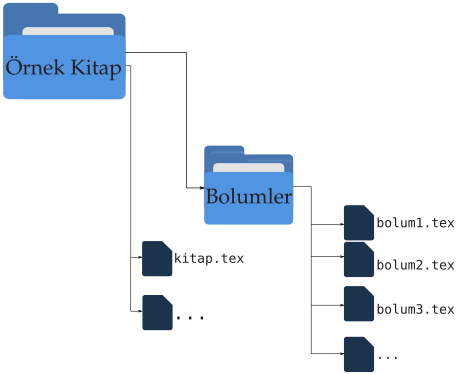
\includegraphics[width=0.5\textwidth,height=\textheight]{images/dizin.png}
\caption{Kaynak dosyanın olduğu dizinin düzenlenmesi}
\end{figure}

Bu şekilde bir düzenleme yaptığınızda \texttt{\textbackslash{}input} ya da \texttt{\textbackslash{}include} komutlarıyla dosya eklemek istediğinizde dosyanın bulunduğu dizini de göstermeniz gerekir.

Burada kaynak dosya \texttt{kitap.tex}'dir. Bu kaynak dosyaya \texttt{bolum1.tex} dosyasını eklemek istediğinizde komutu

\begin{Shaded}
\begin{Highlighting}[]
\FunctionTok{\textbackslash{}input}\NormalTok{\{Bolumler/bolum1\}}
\end{Highlighting}
\end{Shaded}

şeklinde verirsiniz. Bu sayede kaynak dosyanızın olduğu dizinde (Örnek Kitap) sadece \texttt{kitap} ile başlayan dosyalar olur. Diğer dosyalar alt dizinde (Bolumler) yer alır.

Dikkat edilirse ``Örnek Kitap'' dışında, ``Bolumler'' alt dizini ve tüm dosya adları Türkçe karakter ya da boşluk içermez.

\begin{Shaded}
\begin{Highlighting}[]
\BuiltInTok{\textbackslash{}documentclass}\NormalTok{[a4paper,12pt]\{}\ExtensionTok{book}\NormalTok{\}}
\BuiltInTok{\textbackslash{}usepackage}\NormalTok{[T1]\{}\ExtensionTok{fontenc}\NormalTok{\}}
\BuiltInTok{\textbackslash{}usepackage}\NormalTok{[turkish]\{}\ExtensionTok{babel}\NormalTok{\}}
\FunctionTok{\textbackslash{}title}\NormalTok{\{Örnek Kitap\}}
\FunctionTok{\textbackslash{}author}\NormalTok{\{}\FunctionTok{\textbackslash{}TeX}\NormalTok{ dizgi\}}
\KeywordTok{\textbackslash{}begin}\NormalTok{\{}\ExtensionTok{document}\NormalTok{\}}
\FunctionTok{\textbackslash{}frontmatter}
\FunctionTok{\textbackslash{}maketitle}
\FunctionTok{\textbackslash{}tableofcontents}
\FunctionTok{\textbackslash{}input}\NormalTok{\{Bolumler/onsoz\}}
\FunctionTok{\textbackslash{}mainmatter}
\FunctionTok{\textbackslash{}input}\NormalTok{\{Bolumler/bolum1\}}
\FunctionTok{\textbackslash{}input}\NormalTok{\{Bolumler/bolum2\}}
\FunctionTok{\textbackslash{}appendix}
\FunctionTok{\textbackslash{}input}\NormalTok{\{Bolumler/ek1\}}
\FunctionTok{\textbackslash{}backmatter}
\KeywordTok{\textbackslash{}end}\NormalTok{\{}\ExtensionTok{document}\NormalTok{\}}
\end{Highlighting}
\end{Shaded}

\hypertarget{varsayux131lan-sayfa-duxfczenini-deux11fiux15ftirme}{%
\section{Varsayılan Sayfa Düzenini Değiştirme}\label{varsayux131lan-sayfa-duxfczenini-deux11fiux15ftirme}}

LaTeX'de varsayılan kağıt boyutunun \texttt{letterpaper} olduğunu Bölün \ref{belgesinifi}'de ifade etmiştik. Ayrıca aynı yazıda başka bir kağıt boyutunun nasıl seçileceğine de yer vermiştik. Şimdi ise hem sayfamızın kenar boşluklarının nasıl ayarlanacağından hem de ön tanımlı olmayan, tamamen keyfi bir sayfa boyutunun nasıl belirleneceğinden bahsedelim.

Bu tür sayfa düzenlemeleri için LaTeX'de \href{http://ftp.cc.uoc.gr/mirrors/CTAN/macros/latex/contrib/geometry/geometry.pdf}{\textbf{geometry}} paketi kullanılır. Öncelikle paketi

\begin{Shaded}
\begin{Highlighting}[]
\BuiltInTok{\textbackslash{}usepackage}\NormalTok{\{}\ExtensionTok{geometry}\NormalTok{\}}
\end{Highlighting}
\end{Shaded}

komutuyla sahanlığa ekleyin. Ardından paket seçeneklerinde aşağıdaki tanımlamalarla sayfanın düzenini değiştirebilirsiniz:

\begin{longtable}[]{@{}ll@{}}
\toprule
Tanım & Değer \\
\midrule
\endhead
\texttt{top} & üst boșluk \\
\texttt{bottom} & alt boșluk \\
\texttt{left} & sol boșluk \\
\texttt{right} & sağ boșluk \\
\texttt{paperwidht} & sayfa genișliği \\
\texttt{paperheight} & sayfa yüksekliği \\
\bottomrule
\end{longtable}

Örneğin sahanlıkta

\begin{Shaded}
\begin{Highlighting}[]
\BuiltInTok{\textbackslash{}usepackage}\NormalTok{[paperwidth=175mm,paperheight=255mm,top=2cm,bottom=2cm,}
\NormalTok{left=2.5cm,right=2.5cm]\{}\ExtensionTok{geometry}\NormalTok{\}}
\end{Highlighting}
\end{Shaded}

komutunu verdiğinizde boyutu \(175\times 255\) mm, üst ve alt boşluğu \(2\) cm, sol ve sağ boşluğu \(2.5\) cm olan bir sayfa düzeni oluşturursunuz. Dilerseniz \texttt{paperwidth} ve\texttt{paperheight} tanımlamalarını yerine, örneğin \texttt{a4paper} yazarak sadece kenar boşluklarla ilgili tanımlamaları yapabilirsiniz.

\begin{quote}
LaTeX'de milimetre (mm) ve santimetre (cm) dışında inç (in), punto (pt), em ve ex gibi ölçü birimleri de vardır. Bunlara ileride değinilecektir. Ayrıca yine ileride daha ayrıntılı sayfa düzeni oluşturmaktan da bahsedeceğiz. Bu aşamada bu kadarı yeterli olacaktır.
\end{quote}

\hypertarget{satux131r-ve-sayfa-kesme}{%
\section{Satır ve Sayfa Kesme}\label{satux131r-ve-sayfa-kesme}}

LaTeX, kelimeler arası boşlukları otomatik ayarlayarak satırları iki yana yaslayarak dizer. Bir satırı kesip yeni bir satıra geçmek için \texttt{\textbackslash{}\textbackslash{}} veya \texttt{\textbackslash{}newline} komutları kullanılır.

Birinci komut \texttt{\textbackslash{}\textbackslash{}*} şeklinde verildiğinde satırdan sonra sayfa kesilmesini önler.

Benzer şeyi \texttt{\textbackslash{}linebreak} komutu da yapar. Fakat bu komut ile satır kesilirse LaTeX kalan yarım satırı iki yana yaslar. \texttt{\textbackslash{}nolinebreak} komutu ise satırın kesilmesini önler.

Birçok kelimeyi birlikte aynı satırda tutmak gerekirse \texttt{\textbackslash{}mbox} komutu kullanılır:

\begin{Shaded}
\begin{Highlighting}[]
\FunctionTok{\textbackslash{}mbox}\NormalTok{\{\textless{}metin\textgreater{}\}}
\end{Highlighting}
\end{Shaded}

Buradaki \texttt{\textless{}metin\textgreater{}} içindeki kelimeler her durumda birleşik kalırlar. Benzer şeyi \texttt{\textbackslash{}fbox} komutu da metin etrafına çizgi çizerek yapar.

Sayfayı kesip yeni bir sayfaya geçmek için \texttt{\textbackslash{}newpage} ya da \texttt{\textbackslash{}pagebreak} komutları kullanılır. \texttt{\textbackslash{}nopagebreak} komutu sayfa kesilmesini önler. \texttt{\textbackslash{}newpage} ile \texttt{\textbackslash{}pagebreak} komutları arasında da \texttt{\textbackslash{}newline} ile \texttt{\textbackslash{}linebreak} komutlarındakine benzer bir fark vardır.

\hypertarget{paragraflar-ve-cuxfcmle-sonlarux131}{%
\section{Paragraflar ve Cümle Sonları}\label{paragraflar-ve-cuxfcmle-sonlarux131}}

Boş bir satırın yeni bir paragraf açtığını Bölüm \ref{bosluk}'de belirtmiştik. Aynı şey, \texttt{\textbackslash{}par} komutuyla da yapılabilir. Ancak bu komut yeni bir paragraf açmaktan ziyade farklı amaçlar için kullanılır (yeri geldiğinde değinilecektir). Nitekim kaynak dosyanızın okunabilirliği açısından paragrafları ayırmak için boş bir satır bırakmak daha kullanışlıdır.

LaTeX'de varsayılan olarak \texttt{\textbackslash{}chapter} ve \texttt{\textbackslash{}section} gibi bölümleme komutlarından sonra oluşturulan ilk paragraf girintisiz, sonrakiler girintili olur. Bu, paragraf başlarında \texttt{\textbackslash{}indent} ya da \texttt{\textbackslash{}noindent} komutlarıyla tek seferliğine değiştirilebilir. Birinci komut girinti oluşturur, ikincisi ise girintiyi kaldırır.

LaTeX, okumayı kolaylaştırmak için cümle sonlarında fazladan boşluklar bırakır. Bunu yaparken de her cümlenin nokta, soru işareti veya ünlem işaretiyle bittiğini varsayar. Kısaltmalarda büyük harflerden sonra nokta geldiğinden, büyük harften sonra nokta koyulursa LaTeX bunu cümle sonu saymaz. Eğer bir büyük harften sonra nokta koyuyorsanız ve burası cümlenin sonuysa LaTeX'in burayı cümle sonu sayması için büyük harften sonraki noktanın önüne \texttt{\textbackslash{}@} koymanız gerekir.

LaTeX'in noktadan sonra fazladan boşluk \emph{koymamasını} isterseniz \texttt{\textbackslash{}frenchspacing} komutunu kullanırsınız. Bu komutu kullandıysanız, artık noktadan önce \texttt{\textbackslash{}@} koymanıza gerek yoktur. Daha sonra tekrar cümle sonlarında fazladan boşluk kullanmak istenirse de \texttt{\textbackslash{}nonfrenchspacing} komutu kullanılır.

Unvan kısaltmasından sonra unvanın ait olduğu kelimeyle birlikte kalması ve fazladan boşluk bırakılmaması için tilda (\texttt{\textasciitilde{}}) işareti kullanılabilir. Bu işaret hem genişlemeyen bir boşluk bırakır hem de satırın orada kesilmesini önler.

\hypertarget{aralux131klar}{%
\section{Aralıklar}\label{aralux131klar}}

LaTeX'de hem dikey hem de yatay aralıklar otomatik olarak ayarlanır. Fazladan aralıklar bırakmak için komutlar kullanılır.

Aralık bırakırken kullanabileceğimiz ölçü birimleri Tablo \ref{tab:olcubir}'de gösterilmiştir.

\begin{longtable}[]{@{}ll@{}}
\caption{\label{tab:olcubir} LaTeX'de Ölçü Birimleri}\tabularnewline
\toprule
Birim & Değer \\
\midrule
\endfirsthead
\toprule
Birim & Değer \\
\midrule
\endhead
mm & milimetre \(\approx 1/25\) inç \\
cm & santimetre = 10 mm \\
in & inç = 25.4 mm \\
pt & punto \(\approx 1/72\) inç \\
em & Kullanılan yazı tipinde `M' harfinin genişliği \\
ex & Kullanılan yazı tipinde `x' harfinin yüksekliği \\
\bottomrule
\end{longtable}

\hypertarget{dikey-aralux131klar}{%
\subsection{Dikey aralıklar}\label{dikey-aralux131klar}}

Dikey aralık birkaç komutla bırakılabilir. Bunlardan biri \texttt{\textbackslash{}vspace} olup, komut iki boş satır arasında

\begin{Shaded}
\begin{Highlighting}[]
\FunctionTok{\textbackslash{}vspace}\NormalTok{\{\textless{}uzunluk\textgreater{}\}}
\end{Highlighting}
\end{Shaded}

şeklinde verilir. Komut bu şekilde verildiğinde komutun zorunlu değişkeninde birimiyle belirtilen uzunluk kadar dikey aralık bırakılır. Eğer bir sayfanın başında veya sonunda aralık bırakılmak istenirse, komut \texttt{\textbackslash{}vspace*} şeklinde yıldızlı vermelidir. Bu komutun aralığa ilave yapan \texttt{\textbackslash{}addvspace} sürümü de vardır.

Bir paragrafın iki satırı arasında veya bir tablonun satırları arasında ilave aralık açmak için

\begin{Shaded}
\begin{Highlighting}[]
\FunctionTok{\textbackslash{}\textbackslash{}}\NormalTok{[\textless{}uzunluk\textgreater{}]}
\end{Highlighting}
\end{Shaded}

komutu kullanılır.

\begin{Shaded}
\begin{Highlighting}[]
\NormalTok{A}\FunctionTok{\textbackslash{}\textbackslash{}}\NormalTok{[1ex]}
\NormalTok{B}
\end{Highlighting}
\end{Shaded}

Bu komutlarda belirtilen uzunluklar negatif de olabilir.

\begin{Shaded}
\begin{Highlighting}[]
\NormalTok{A}\FunctionTok{\textbackslash{}\textbackslash{}}\NormalTok{[{-}2ex]}
\NormalTok{B}
\end{Highlighting}
\end{Shaded}

Sınırsız bir dikey aralık oluşturmak için \texttt{\textbackslash{}vfill} komutu kullanılır. Bu komuttan sonra gelen her şey sayfanın altına yaslanır.

Ön tanımlı gelen \texttt{\textbackslash{}smallskip}, \texttt{\textbackslash{}medskip} ve \texttt{\textbackslash{}bigskip} komutları sırasıyla küçük, orta ve büyük aralıklar bırakır.

\hypertarget{yatay-aralux131klar}{%
\subsection{Yatay aralıklar}\label{yatay-aralux131klar}}

Ön tanımlı yatay aralıklar

\begin{Shaded}
\begin{Highlighting}[]
\FunctionTok{\textbackslash{} } \FunctionTok{\textbackslash{},}  \FunctionTok{\textbackslash{}:}  \FunctionTok{\textbackslash{};}  \FunctionTok{\textbackslash{}quad}  \FunctionTok{\textbackslash{}qquad}  \FunctionTok{\textbackslash{}!}
\end{Highlighting}
\end{Shaded}

komutlarıyla verilir. Bu komutlar sırasıyla bir sözcük arası, \(3/\!18\) em, \(4/\!18\) em, \(5/\!18\) em, \(1\) em, \(2\) em, \(-3/\!18\) em uzunlukta yatay aralık bırakır.

Belli bir uzunlukta yatay aralık bırakmak için \texttt{\textbackslash{}hspace} komutu kullanılır. Yine dikey aralıkta olduğu gibi yatay aralık negatif de olabilir. Eğer aralık satır başına veya sonuna rasgelse dahi bu aralığı korumak istiyorsanız, yıldızlı \texttt{\textbackslash{}hspace*} komutu kullanırsınız.

\begin{Shaded}
\begin{Highlighting}[]
\NormalTok{A}\FunctionTok{\textbackslash{}hspace}\NormalTok{\{2cm\}B}\FunctionTok{\textbackslash{}\textbackslash{}}
\NormalTok{A }\FunctionTok{\textbackslash{}hspace}\NormalTok{\{2cm\} B}
\end{Highlighting}
\end{Shaded}

Komutlardan önce veya sonra boşluk bırakmak farklı sonuçlar üretir.

Sınırsız bir yatay aralık oluşturmak için \texttt{\textbackslash{}hfill} komutu kullanılır. Bu komuttan sonra gelen her şey satırın sonuna yaslanır. Hem satır sonuna yaslamak hem de aralığı noktalarla doldurmak isterseniz \texttt{\textbackslash{}dotfill} komutunu kullanırsınız. Satır sonuna yaslayıp aralığa çizgi çekmek isterseniz de \texttt{\textbackslash{}hrulefill} komutunu kullanırsınız.

\begin{Shaded}
\begin{Highlighting}[]
\NormalTok{A}\FunctionTok{\textbackslash{}hfill}\NormalTok{ B}\FunctionTok{\textbackslash{}\textbackslash{}}
\NormalTok{A}\FunctionTok{\textbackslash{}dotfill}\NormalTok{ B}\FunctionTok{\textbackslash{}\textbackslash{}}
\NormalTok{A}\FunctionTok{\textbackslash{}hrulefill}\NormalTok{ B}
\end{Highlighting}
\end{Shaded}

\hypertarget{metni-hizalamak-ve-suxfctunlara-buxf6lmek}{%
\section{Metni Hizalamak ve Sütunlara Bölmek}\label{metni-hizalamak-ve-suxfctunlara-buxf6lmek}}

\hypertarget{hizalama}{%
\subsection{Hizalama}\label{hizalama}}

LaTeX'de metni sola hizalamak için \texttt{flushleft}, sağa hizalamak için \texttt{flushright} ve ortalı hizalamak için \texttt{center} ortamları kullanılır.

\begin{Shaded}
\begin{Highlighting}[]
\KeywordTok{\textbackslash{}begin}\NormalTok{\{}\ExtensionTok{flushleft}\NormalTok{\}}
\NormalTok{ burası sola hizalı}
\KeywordTok{\textbackslash{}end}\NormalTok{\{}\ExtensionTok{flushleft}\NormalTok{\}}
\KeywordTok{\textbackslash{}begin}\NormalTok{\{}\ExtensionTok{flushright}\NormalTok{\}}
\NormalTok{ sağa hizalı}
\KeywordTok{\textbackslash{}end}\NormalTok{\{}\ExtensionTok{flushright}\NormalTok{\}}
\KeywordTok{\textbackslash{}begin}\NormalTok{\{}\ExtensionTok{center}\NormalTok{\}}
\NormalTok{ ve ortalı}
\KeywordTok{\textbackslash{}end}\NormalTok{\{}\ExtensionTok{center}\NormalTok{\}}
\end{Highlighting}
\end{Shaded}

\hypertarget{suxfctunlara-buxf6lmek}{%
\subsection{Sütunlara bölmek}\label{suxfctunlara-buxf6lmek}}

LaTeX'de belgenin tamamının iki sütun dizilmesi için \texttt{\textbackslash{}documentclass} komutunun seçeneğine \texttt{twocolumn} yazılabileceğinden Bölüm \ref{belgesinifi}'de bahsettik. Bu, tüm belgenin iki sütun dizilmesini sağlar. Bazı sayfaları iki, bazılarınıysa tek sütun dizmek istiyorsanız \texttt{\textbackslash{}twocolumn} ve \texttt{\textbackslash{}onecolumn} komutlarını kullanmanız gerekir. \texttt{\textbackslash{}twocolumn} komutunun verildiği sayfadan sonraki sayfalar iki, \texttt{\textbackslash{}onecolumn} komutunun verildiği sayfadan sonraki sayfalar tek sütun dizilir.

Eğer metni daha fazla sütuna bölmek ve sütunları istediğiniz yerden başlatmak gibi daha fazla seçenek istiyorsanız, \texttt{multicols} ortamını kullanmanız gerekir. Bu ortamı kullanabilmek için

\begin{Shaded}
\begin{Highlighting}[]
\BuiltInTok{\textbackslash{}usepackage}\NormalTok{\{}\ExtensionTok{multicol}\NormalTok{\}}
\end{Highlighting}
\end{Shaded}

komutuyla \href{http://ftp.ntua.gr/mirror/ctan/macros/latex/required/tools/multicol.pdf}{\textbf{multicol}} paketini eklemelisiniz.

\begin{Shaded}
\begin{Highlighting}[]
\KeywordTok{\textbackslash{}begin}\NormalTok{\{}\ExtensionTok{multicols}\NormalTok{\}\{\textless{}sütun sayısı\textgreater{}\}}

\KeywordTok{\textbackslash{}end}\NormalTok{\{}\ExtensionTok{multicols}\NormalTok{\}}
\end{Highlighting}
\end{Shaded}

Burada, \texttt{\textless{}sütun\ sayısı\textgreater{}} değişkeninde oluşturulmak istenen sütun adedi sayıyla belirtilir.

Bu ortamda sütun genişlikleri eşit olup, sütunlar arası boşluk \texttt{\textbackslash{}columnsep}, sütunlar arasındaki çizginin kalınlığı \texttt{\textbackslash{}columnseprule} ve sütunlar arasındaki çizginin rengi \texttt{\textbackslash{}columnseprulecolor} komutlarında saklıdır. Bu değişkenler \texttt{\textbackslash{}setlength} ya da \texttt{\textbackslash{}def} komutları kullanılarak değiştirilebilir.

\begin{Shaded}
\begin{Highlighting}[]
\FunctionTok{\textbackslash{}setlength}\NormalTok{\{}\FunctionTok{\textbackslash{}columnsep}\NormalTok{\}\{1cm\}}
\FunctionTok{\textbackslash{}setlength}\NormalTok{\{}\FunctionTok{\textbackslash{}columnseprule}\NormalTok{\}\{1pt\}}
\FunctionTok{\textbackslash{}def\textbackslash{}columnseprulecolor}\NormalTok{\{}\FunctionTok{\textbackslash{}color}\NormalTok{\{blue\}\}}
\end{Highlighting}
\end{Shaded}

Yukarıdaki birinci komutla sütunlar arasındaki boşluk 1 cm, çizgi kalınlığı 1 pt ve çizgi rengi mavi olarak düzenlenir. Bu komutlar ya sahanlığa ya da ortamı kullanmadan önce gövdeye yazılmalıdır.

\begin{quote}
Şimdiye kadar renk kullanımından bahsetmedik ancak çizgi rengini değiştirmek için verilen komutun kullanılabilmesi için sahanlığa \texttt{\textbackslash{}usepackage\{color\}} komutuyla \texttt{color} paketinin eklenmesi gerekir.
\end{quote}

Ortam isteğe bağlı bir değişken de alabilir. Bu, çengelli parantezlerden sonra köşeli parantezler içine yazılır. Köşeli parantezler içinde yazılanlar bölünmeden ve çok sütunlu metnin üstünde dizilir.

\begin{Shaded}
\begin{Highlighting}[]
\KeywordTok{\textbackslash{}begin}\NormalTok{\{}\ExtensionTok{multicols}\NormalTok{\}\{2\}}
\NormalTok{ [}\KeywordTok{\textbackslash{}section}\NormalTok{\{Başlık\}}
\NormalTok{ Burası sütunlara bölünmez.]}
\NormalTok{ Burası sütunlara bölünür.}
\KeywordTok{\textbackslash{}end}\NormalTok{\{}\ExtensionTok{multicols}\NormalTok{\}}
\end{Highlighting}
\end{Shaded}

Sütunu kesmek için \texttt{\textbackslash{}columnbreak} komutu kullanılır. Komutun verildiği yerde sütun kesilir, ardından kesme noktasından önceki paragraflar tüm kullanılabilir alanı doldurmak için eşit olarak dağıtılır. Dolayısıyla bazen beklenen sonucu vermeyebilir.

Varsayılan \texttt{multicols} ortamında sütunların her biri aynı miktarda metin içerecek şekilde dengelenmiştir. Bu, ortamın yıldızlı sürümü (\texttt{multicols*}) kullanılarak değiştirilebilir.

\hypertarget{listeleme}{%
\section{Listeleme}\label{listeleme}}

\hypertarget{temel-listeler}{%
\subsection{Temel listeler}\label{temel-listeler}}

LaTeX'de listeleme için değişik ortamlar vardır. Bu ortamlar tek başına kullanılabileceği gibi birlikte de kullanılabilirler. Her ortamda maddeler \texttt{\textbackslash{}item} komutuyla belirtilir.

Bir listeyi numaralı şekilde dizmek için \texttt{enumerate} ortamı kullanılır.

\begin{Shaded}
\begin{Highlighting}[]
\KeywordTok{\textbackslash{}begin}\NormalTok{\{}\ExtensionTok{enumerate}\NormalTok{\}}
 \FunctionTok{\textbackslash{}item}\NormalTok{ madde 1}
  \KeywordTok{\textbackslash{}begin}\NormalTok{\{}\ExtensionTok{enumerate}\NormalTok{\}}
    \FunctionTok{\textbackslash{}item}\NormalTok{ alt madde 1}
      \KeywordTok{\textbackslash{}begin}\NormalTok{\{}\ExtensionTok{enumerate}\NormalTok{\}}
        \FunctionTok{\textbackslash{}item}\NormalTok{ en alt madde 1}
      \KeywordTok{\textbackslash{}end}\NormalTok{\{}\ExtensionTok{enumerate}\NormalTok{\}}
    \FunctionTok{\textbackslash{}item}\NormalTok{ alt madde 2}
  \KeywordTok{\textbackslash{}end}\NormalTok{\{}\ExtensionTok{enumerate}\NormalTok{\}}
 \FunctionTok{\textbackslash{}item}\NormalTok{ madde 2}
\KeywordTok{\textbackslash{}end}\NormalTok{\{}\ExtensionTok{enumerate}\NormalTok{\}}
\end{Highlighting}
\end{Shaded}

\insvg


\includegraphics{examples/ex3.svg} \outsvg

Numarasız, özel işaretli listeler için \texttt{itemize} ortamı kullanılır ve bu ortamda madde işareti değiştirilebilir.

\begin{Shaded}
\begin{Highlighting}[]
\KeywordTok{\textbackslash{}begin}\NormalTok{\{}\ExtensionTok{itemize}\NormalTok{\}}
\FunctionTok{\textbackslash{}item}\NormalTok{ madde 1}
\FunctionTok{\textbackslash{}item}\NormalTok{ madde 2}
\FunctionTok{\textbackslash{}item}\NormalTok{[}\SpecialStringTok{$}\SpecialCharTok{\textbackslash{}circ}\SpecialStringTok{$}\NormalTok{] madde 3}
\FunctionTok{\textbackslash{}item}\NormalTok{[+] madde 4}
\KeywordTok{\textbackslash{}end}\NormalTok{\{}\ExtensionTok{itemize}\NormalTok{\}}
\end{Highlighting}
\end{Shaded}

Açıklamalı bir liste içinse \texttt{description} ortamı kullanılır. Bu ortamda köşeli parantez içine alınan anahtar kelimeler kalın dizilir.

\begin{Shaded}
\begin{Highlighting}[]
\KeywordTok{\textbackslash{}begin}\NormalTok{\{}\ExtensionTok{description}\NormalTok{\}}
  \FunctionTok{\textbackslash{}item}\NormalTok{[Nokta] Boyutu olmayan}
  \FunctionTok{\textbackslash{}item}\NormalTok{[Çember] Bir noktaya eşit}
\NormalTok{  uzaklıktaki noktaların geometrik yeri}
\KeywordTok{\textbackslash{}end}\NormalTok{\{}\ExtensionTok{description}\NormalTok{\}}
\end{Highlighting}
\end{Shaded}

\hypertarget{listeleri-uxf6zelleux15ftirmek}{%
\subsection{Listeleri özelleştirmek}\label{listeleri-uxf6zelleux15ftirmek}}

Listelerin özelleştirmek için \href{http://ftp.ntua.gr/mirror/ctan/macros/latex/required/tools/enumerate.pdf}{\textbf{enumerate}} paketi kullanılabilir. Paketi \texttt{\textbackslash{}usepackage\{enumerate\}} komutuyla ekledikten sonra \texttt{enumerate} ortamını başlatan komutun peşine köşeli parantezler içinde madde işaretlerinin tipi belirtilebilir:

\begin{Shaded}
\begin{Highlighting}[]
\KeywordTok{\textbackslash{}begin}\NormalTok{\{}\ExtensionTok{enumerate}\NormalTok{\}[I.]}
 \FunctionTok{\textbackslash{}item}\NormalTok{ bir}
 \FunctionTok{\textbackslash{}item}\NormalTok{ iki }
 \FunctionTok{\textbackslash{}item}\NormalTok{ üç}
\KeywordTok{\textbackslash{}end}\NormalTok{\{}\ExtensionTok{enumerate}\NormalTok{\}}
\end{Highlighting}
\end{Shaded}

Bunun dışında çok daha fazla özelleştirmeye izin veren \href{http://ftp.cc.uoc.gr/mirrors/CTAN/macros/latex/contrib/enumitem/enumitem.pdf}{\textbf{enumitem}} paketi vardır. Bu paketi kullanarak yapılabilecek listelere de ilerde değineceğiz. Dileyen okur paket belgesini inceleyip listelerini özelleştirebilir.

\hypertarget{yazux131tipleri}{%
\section{Yazıtipleri}\label{yazux131tipleri}}

\hypertarget{giriux15f}{%
\subsection{Giriş}\label{giriux15f}}

Yazıtipi konusu \emph{kodlama}, \emph{aile}, \emph{biçem} ve \emph{boyut} olmak üzere dört alt başlıkta incelenebilir. Kodlama çok teknik bir konu olup amacımız dışındadır, ancak sadece şunu belirtelim ki kodlama işini LaTeX'de Bölüm \ref{turkce}'de bahsettiğimiz \textbf{fontenc} paketi üstlenir. Bu paketi belgenize eklemiş olduğunuzu varsayarak devam edeceğiz.

Bu yazıda anlatacağımız şeylerden bazıları bir bakıma LaTeX'in felsefesine aykırı olacak. Nitekim LaTeX, \texttt{\textbackslash{}documentclass} komutunda belirtilen ana yazıtipi boyutuna göre, dipnot ya da başlık gibi ana yazıtipi boyutundan farklı dizilen şeylerin boyutunu olabilecek en güzel ve doğru şekilde ayarlar. O yüzden bu konudaki klasik uyarıyı biz de yineleyelim:


\includegraphics[width=1\textwidth,height=\textheight]{images/uyari.png}

\hypertarget{aile}{%
\subsection{Aile}\label{aile}}

Yazıtipleri Roman ya da Serif, Sans Serif ve Typewriter olmak üzere üç ailede toplanabilir. Roman ailesi tırnaklı ya da süslü diyebileceğimiz yazıtiplerini, Sans Serif ailesi tırnaksız ya da süssüz yazıtiplerini ve Typewriter ailesi de daktilo yazıtiplerini barındırır.

LaTeX'de her belge sınıfı varsayılan yazıtipi ailesiyle gelir. \texttt{beamer} sınıfının varsayılan ailesi Sans Serif olup, diğer sınıfların varsayılan ailesi Roman'dır.

Varsayılan aile \texttt{\textbackslash{}familydefault} komutunda saklı olup, \texttt{\textbackslash{}renewcommand} komutuyla değiştirilebilir.

\begin{Shaded}
\begin{Highlighting}[]
\FunctionTok{\textbackslash{}renewcommand}\NormalTok{\{}\ExtensionTok{\textbackslash{}familydefault}\NormalTok{\}\{}\FunctionTok{\textbackslash{}rmdefault}\NormalTok{\}  }
\FunctionTok{\textbackslash{}renewcommand}\NormalTok{\{}\ExtensionTok{\textbackslash{}familydefault}\NormalTok{\}\{}\FunctionTok{\textbackslash{}sfdefault}\NormalTok{\}  }
\FunctionTok{\textbackslash{}renewcommand}\NormalTok{\{}\ExtensionTok{\textbackslash{}familydefault}\NormalTok{\}\{}\FunctionTok{\textbackslash{}ttdefault}\NormalTok{\} }
\end{Highlighting}
\end{Shaded}

Birinci komut sahanlığa yazılırsa, belge sınıfından bağımsız olarak varsayılan aile Roman, ikincisi yazılırsa Sans Serif, üçüncüsü yazılırsa Typewriter olur.

Eğer belgenin tamamının değilde bazı kelime ya da cümlelerin farklı aileden yazılması istenirse --ki genelde böyle kullanılır-- aşağıdaki komut ya da bildirimler kullanılır.

\begin{figure}
\centering
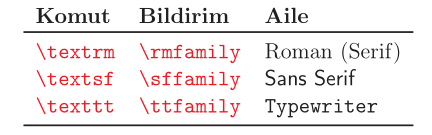
\includegraphics[width=0.5\textwidth,height=\textheight]{images/yazitipi.png}
\caption{Yazıtipi Aileleri}
\end{figure}

LaTeX'de varsayılan yazıtipi Computer Modern olup, ek bir pakete ihtiyaç duymadan kullanılabilecek yazıtipleri aşağıda gösterilmiştir.

\begin{figure}
\centering
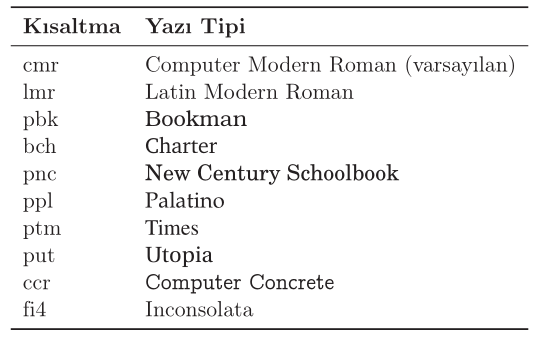
\includegraphics[width=0.5\textwidth,height=\textheight]{images/yazitipi2.png}
\caption{Roman Yazıtipleri}
\end{figure}

\begin{figure}
\centering
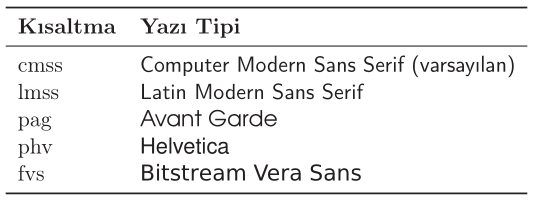
\includegraphics[width=0.5\textwidth,height=\textheight]{images/yazitipi3.png}
\caption{Sans Serif Yazıtipleri}
\end{figure}

\begin{figure}
\centering
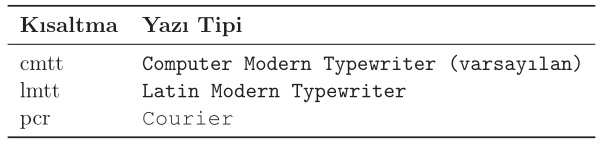
\includegraphics[width=0.5\textwidth,height=\textheight]{images/yazitipi4.png}
\caption{Typewriter Yazıtipleri\\
}
\end{figure}

\begin{figure}
\centering
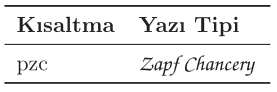
\includegraphics[width=0.25\textwidth,height=\textheight]{images/yazitipi5.png}
\caption{Elyazısı}
\end{figure}

Varsayılan yazıtipleri \texttt{\textbackslash{}rmdefault}, \texttt{\textbackslash{}sfdefault} ve \texttt{\textbackslash{}ttdefault} komutlarında saklı olup, \texttt{\textbackslash{}renewcommand} komutuyla değiştirilebilirler.

\begin{verbatim}
\renewcommand{\rmdefault}{<kısaltma>}
\end{verbatim}

Burada \texttt{\textless{}kısaltma\textgreater{}}, tablolarda belirtilen kısaltmalardır. Örneğin

\begin{verbatim}
\renewcommand{\rmdefault}{put}
\end{verbatim}

komutu sahanlığa yazıldığında, eğer varsayılan aile Roman ise belgenizin ana yazıtipi Utopia olur.

Eğer tüm belgenin değil, bazı kelime ya da cümlelerin farklı yazıtipinde yazılması istenirse \texttt{\textbackslash{}fontfamily} komutuyla \texttt{\textbackslash{}selectfont} komutu birlikte aşağıdaki şekilde kullanılır.

\begin{verbatim}
{\fontfamily{pbk}\selectfont Bookman yazıtipi.} Ana yazıtipi.
\end{verbatim}

Varsayılan yazıtipi paket ekleyerek de değiştirilebilir. Bu hem pratiktir hem de bazı paketler matematiksel ifadelerin yazıtipine de etki eder. Bu paketlerin bazıları tabloda gösterilmiştir.

\begin{figure}
\centering
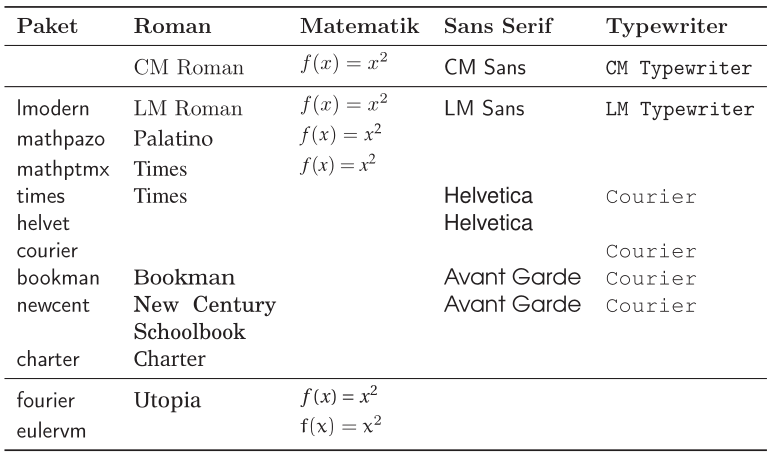
\includegraphics[width=0.7\textwidth,height=\textheight]{images/yazitipi6.png}
\caption{Yazıtipi değiştiren paketler}
\end{figure}

Bunların dışında beğenebileceğiniz birçok yazıtipini \href{https://tug.org/FontCatalogue/}{LaTeX Yazıtipi Kataloğu}'nda bulabilirsiniz.

\hypertarget{biuxe7em}{%
\subsection{Biçem}\label{biuxe7em}}

Metin içinde kelimeleri bazen italik bazen de kalın dizmek isteyebilirsiniz. Bu değişimler aşağıdaki tablodaki komut ya da bildirimlerle yapılır.

\begin{figure}
\centering
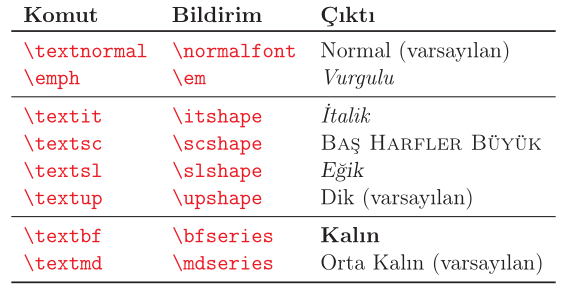
\includegraphics[width=0.5\textwidth,height=\textheight]{images/yazitipi7.png}
\caption{Yazıtipi Biçemleri}
\end{figure}

\begin{Shaded}
\begin{Highlighting}[]
\NormalTok{İzleyen kelime }\FunctionTok{\textbackslash{}textit}\NormalTok{\{italik\} }
\NormalTok{harflerle yazılmıştır.}
\NormalTok{Metnin geri kalan kısmı}
\NormalTok{normaldir.}
\end{Highlighting}
\end{Shaded}

\begin{Shaded}
\begin{Highlighting}[]
\NormalTok{İzleyen ifade \{}\FunctionTok{\textbackslash{}slshape}\NormalTok{ \{}\FunctionTok{\textbackslash{}bfseries}\NormalTok{ eğik kalındır\}\}.}
\end{Highlighting}
\end{Shaded}

\begin{Shaded}
\begin{Highlighting}[]
\NormalTok{İzleyen ifade }\FunctionTok{\textbackslash{}textit}\NormalTok{\{}\FunctionTok{\textbackslash{}textbf}\NormalTok{\{italik kalın\}\}, ama bu}
\FunctionTok{\textbackslash{}textsc}\NormalTok{\{}\FunctionTok{\textbackslash{}textit}\NormalTok{\{büyük küçük harf değil\}\}.}
\end{Highlighting}
\end{Shaded}

Eğer vurgulu metin içinde bazı kelimeler tekrar vurgulanırsa bu kelimeler normale döner.

\begin{Shaded}
\begin{Highlighting}[]
\NormalTok{\{}\FunctionTok{\textbackslash{}em}\NormalTok{ Vurgulu metinde tekrar}
\NormalTok{vurgu yapılırsa \{}\FunctionTok{\textbackslash{}em}\NormalTok{ normale\}}
\NormalTok{döner.\}}
\end{Highlighting}
\end{Shaded}

LaTeX'de vurgu yukarıdaki gibi yapılsa da altını çizerek vurgu yapmak isteyen olabilir. Kuyruklu harflerin altı çizildiğinde varsayılan satır aralığı değiştiğinden vurguyu bu şekilde yapmamanız daha doğrudur. Ancak illa altını çizmek isterseniz \texttt{\textbackslash{}underline} komutunu kullanabilirsiniz.

\hypertarget{boyut}{%
\subsection{Boyut}\label{boyut}}

Yazıtipi boyutunu değiştirmek için aşağıdaki bildirimler kullanılır.

\begin{figure}
\centering
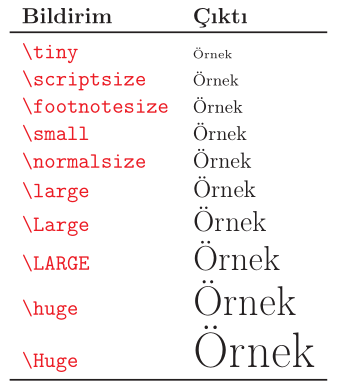
\includegraphics[width=0.5\textwidth,height=\textheight]{images/yazitipi8.png}
\caption{Yazıtipi Boyutu Değiştiren Bildirimler}
\end{figure}

\begin{Shaded}
\begin{Highlighting}[]
\NormalTok{\{}\FunctionTok{\textbackslash{}Large}\NormalTok{ Büyük\} ve}
\NormalTok{\{}\FunctionTok{\textbackslash{}scriptsize}\NormalTok{ küçük\} harfler.}
\end{Highlighting}
\end{Shaded}

Bu bildirimlerin aynı zamanda satır aralığını da değiştirdiğine dikkat edilmelidir. Aşağıdaki iki örnekte, \texttt{\textbackslash{}par} (paragraf) komutunun verdiğiniz yere bağlı olarak farklı sonuçlar ürettiği gösterilmiştir. Doğru kullanım ikincisidir.

\begin{Shaded}
\begin{Highlighting}[]
\NormalTok{\{}\FunctionTok{\textbackslash{}large} 
\NormalTok{Sokrates: Platon}
\NormalTok{yalan söyleyecek}
\NormalTok{aşağıdaki cümlede.\}}\FunctionTok{\textbackslash{}par}
\end{Highlighting}
\end{Shaded}

\begin{Shaded}
\begin{Highlighting}[]
\NormalTok{\{}\FunctionTok{\textbackslash{}large}\NormalTok{ Platon: Sokrates}
\NormalTok{doğruyu söyledi}
\NormalTok{önceki cümlede.}\FunctionTok{\textbackslash{}par}\NormalTok{\}}
\end{Highlighting}
\end{Shaded}

Bu bildirimlerin etkisi belge ana yazıtipi boyutuna bağımlıdır. Mutlak boyutlar aşağıdaki tabloda gösterilmiştir.

\begin{figure}
\centering
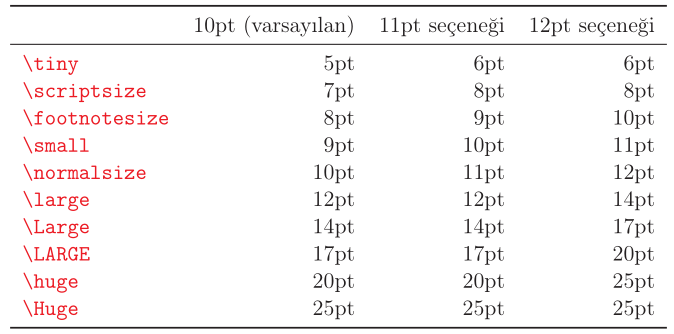
\includegraphics[width=0.7\textwidth,height=\textheight]{images/yazitipi9.png}
\caption{Yazıtipleri Mutlak Boyutları}
\end{figure}

Bağımsız bir yazıtipi boyutu elde etmek için \texttt{\textbackslash{}fontsize} ile \texttt{\textbackslash{}selectfont} komutları birlikte kullanılır.

\begin{Shaded}
\begin{Highlighting}[]
\NormalTok{\{}\FunctionTok{\textbackslash{}fontsize}\NormalTok{\{\textless{}boyut\textgreater{}\}\{\textless{}aralık\textgreater{}\}}\FunctionTok{\textbackslash{}selectfont}\NormalTok{ \textless{}metin\textgreater{}\}}
\end{Highlighting}
\end{Shaded}

Buradaki \texttt{\textless{}boyut\textgreater{}} yazıtipi boyutu, \texttt{\textless{}aralık\textgreater{}} ise satır aralığıdır. İkisinin de ölçü birimi punto (pt) olup, temel kural, aralığın boyutun \(1.2\) katı olmasıdır.

\begin{Shaded}
\begin{Highlighting}[]
\NormalTok{\{}\FunctionTok{\textbackslash{}fontsize}\NormalTok{\{30\}\{36\}}\FunctionTok{\textbackslash{}selectfont}
\NormalTok{Yazı tipi boyutu 30 punto,}
\NormalTok{satır aralığı 36 punto.\}}
\end{Highlighting}
\end{Shaded}

Ana yazıtipi boyutu \texttt{\textbackslash{}normalsize} komutunda saklı olup, \texttt{\textbackslash{}renewcommand} komutuyla değiştirilebilir.

\begin{Shaded}
\begin{Highlighting}[]
\FunctionTok{\textbackslash{}renewcommand}\NormalTok{\{}\ExtensionTok{\textbackslash{}normalsize}\NormalTok{\}\{}\FunctionTok{\textbackslash{}fontsize}\NormalTok{\{30\}\{36\}}\FunctionTok{\textbackslash{}selectfont}\NormalTok{\}}
\end{Highlighting}
\end{Shaded}

Yukarıdaki komutu sahanlığa yazarsanız belgenizin ana yazıtipi boyutu 30 pt, satır aralığı ise 36 pt olur.

\hypertarget{renk-kullanmak}{%
\section{Renk Kullanmak}\label{renk-kullanmak}}

LaTeX'de renkler \href{http://ftp.cc.uoc.gr/mirrors/CTAN/macros/latex/required/graphics/color.pdf}{\textbf{color}} ya da \href{http://ftp.ntua.gr/mirror/ctan/macros/latex/contrib/xcolor/xcolor.pdf}{\textbf{xcolor}} paketleriyle kullanılır. İkinci paket daha güçlüdür.

\begin{Shaded}
\begin{Highlighting}[]
\BuiltInTok{\textbackslash{}usepackage}\NormalTok{\{}\ExtensionTok{xcolor}\NormalTok{\}}
\end{Highlighting}
\end{Shaded}

komutuyla paketi ekledikten sonra \texttt{\textbackslash{}color} ya da \texttt{\textbackslash{}textcolor} komutları aşağıdaki şekillerde kullanılır.

\begin{Shaded}
\begin{Highlighting}[]
\FunctionTok{\textbackslash{}color}\NormalTok{\{red\}\{Kırmızı\}}\FunctionTok{\textbackslash{}\textbackslash{}}
\NormalTok{\{}\FunctionTok{\textbackslash{}color}\NormalTok{\{blue\} Tamamı mavi\}}\FunctionTok{\textbackslash{}\textbackslash{}}
\FunctionTok{\textbackslash{}textcolor}\NormalTok{\{pink\}\{Pembe\}}
\end{Highlighting}
\end{Shaded}

Kullanılabilecek renk adları black, white, gray, darkgray, lightgray, brown, red, green, blue, cyan, magenta, lime, olive, orange, pink, purple, teal, violet ve yellow'dur.

Eğer \texttt{\textbackslash{}documentclass} komutunun seçeneğine \texttt{divpsnames} yazılırsa aşağıdaki renkler de kullanılabilir duruma gelir.

\begin{figure}
\centering
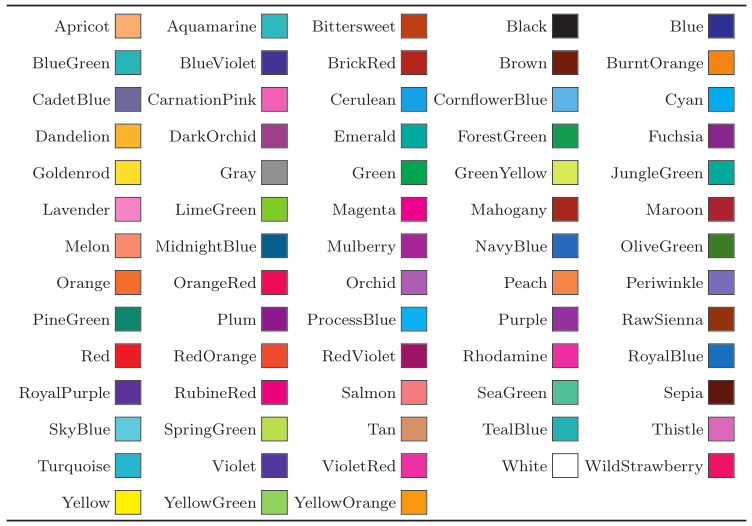
\includegraphics[width=1\textwidth,height=\textheight]{images/renkler.png}
\caption{\textbf{dvipsnames} seçeneğiyle gelen renkler}
\end{figure}

Bunlar da yeterli gelmiyorsa seçeneklere bir de \texttt{svgnames} yazın ve \href{https://www.latextemplates.com/svgnames-colors}{buradaki} yüzden fazla rengi kullanılabilir duruma getirin.

\begin{Shaded}
\begin{Highlighting}[]
\BuiltInTok{\textbackslash{}documentclass}\NormalTok{[svgnames,dvipsnames]\{}\ExtensionTok{article}\NormalTok{\}}
\end{Highlighting}
\end{Shaded}

\hypertarget{yeni-renkler-oluux15fturmak}\NormalTok{80 mavi }\FunctionTok{\textbackslash{}\%}\NormalTok{20 beyaz\}}\FunctionTok{\textbackslash{}\textbackslash{}}
\FunctionTok{\textbackslash{}color}\NormalTok{\{red!40!blue\}\{}\FunctionTok{\textbackslash{}\%}\NormalTok{40 kırmızı }\FunctionTok{\textbackslash{}\%}\NormalTok{60 mavi\} }\FunctionTok{\textbackslash{}\textbackslash{}}
\NormalTok{\{}\FunctionTok{\textbackslash{}color}\NormalTok{\{yellow!20!green!75!black\} }\FunctionTok{\textbackslash{}\%}\NormalTok{20x0.75=15 sarı}
\FunctionTok{\textbackslash{}\%}\NormalTok{(100{-}20)x0.75=60 yeşil }\FunctionTok{\textbackslash{}\%}\NormalTok{100{-}75=25 siyah\}}
\end{Highlighting}
\end{Shaded}

İkinci yol \texttt{\textbackslash{}definecolor} komutuyla renk modelleri kullanmaktır.

\begin{longtable}[]{@{}
  >{\raggedright\arraybackslash}p{(\columnwidth - 2\tabcolsep) * \real{0.5000}}
  >{\raggedright\arraybackslash}p{(\columnwidth - 2\tabcolsep) * \real{0.5000}}@{}}
\caption{\label{tab:renkmod} Renk Modelleri}\tabularnewline
\toprule
\begin{minipage}[b]{\linewidth}\raggedright
\textbf{Model}
\end{minipage} & \begin{minipage}[b]{\linewidth}\raggedright
\textbf{Açıklama}
\end{minipage} \\
\midrule
\endfirsthead
\toprule
\begin{minipage}[b]{\linewidth}\raggedright
\textbf{Model}
\end{minipage} & \begin{minipage}[b]{\linewidth}\raggedright
\textbf{Açıklama}
\end{minipage} \\
\midrule
\endhead
gray & Grinin tonları (0-1). 0 (siyah), 1 (beyaz). Yani 0.95 çok açık gri, 0.30 koyu gri olur. \\
rgb & Red, Green, Blue (0-1). Üç renk (kırmızı, yeșil, mavi) 0 ile 1 arasında bir sayıyla temsil edilir. \\
RGB & Red, Green, Blue (0-255). Üç renk (karmızı, yeșil, mavi) 0 ile 255 arasında bir sayıyla temsil edilir. \\
HTML & Red, Green, Blue (OO-FF). Kodlar RRGGBB şeklinde verilir. \\
cmyk & Cyan, Magenta, Yellow, Black (0-1). Dört renk (camgöbeği, eflatun, sarı, siyah) 0 ile 1 arasında bir sayıyla temsil edilir. \\
\bottomrule
\end{longtable}

Komut

\begin{Shaded}
\begin{Highlighting}[]
\FunctionTok{\textbackslash{}definecolor}\NormalTok{\{\textless{}isim\textgreater{}\}\{\textless{}renk modeli\textgreater{}\}\{\textless{}kod\textgreater{}\}}
\end{Highlighting}
\end{Shaded}

şeklinde verilir. Burada \texttt{\textless{}isim\textgreater{}}, sizin daha sonra kullanmak üzere vereceğiniz bir isimdir. Kodlar için \href{https://www.huesnap.com/color}{HueSnap} adresinden yararlanabilirsiniz. Örneğin

\begin{Shaded}
\begin{Highlighting}[]
\FunctionTok{\textbackslash{}definecolor}\NormalTok{\{renk1\}\{gray\}\{0.50\}}
\FunctionTok{\textbackslash{}definecolor}\NormalTok{\{renk2\}\{rgb\}\{1,0.7,0.3\}}
\FunctionTok{\textbackslash{}definecolor}\NormalTok{\{renk3\}\{RGB\}\{125,32,200\}}
\FunctionTok{\textbackslash{}definecolor}\NormalTok{\{renk4\}\{HTML\}\{CC33CC\}}
\FunctionTok{\textbackslash{}definecolor}\NormalTok{\{renk5\}\{cmyk\}\{0,0.7,1,0.5\}}
\end{Highlighting}
\end{Shaded}

komutlarıyla \texttt{renk1}, \texttt{renk2}, \texttt{renk3}, \texttt{renk4} ve \texttt{renk5} adında beş adet renk tanımlanmış olur. Bu komutlar ya sahanlığa ya da bu renkleri kullanacağınız satırdan önce gövdeye yazılmalıdır.

Yeni oluşturduğunuz rengi tek seferlik kullanacaksanız

\begin{Shaded}
\begin{Highlighting}[]
\FunctionTok{\textbackslash{}color}\NormalTok{[\textless{}model\textgreater{}]\{\textless{}kod\textgreater{}\}}
\FunctionTok{\textbackslash{}textcolor}\NormalTok{[\textless{}model\textgreater{}]\{\textless{}kod\textgreater{}\}\{\textless{}metin\textgreater{}\}}
\end{Highlighting}
\end{Shaded}

komutlarını kullanabilirsiniz.

\begin{Shaded}
\begin{Highlighting}[]
\NormalTok{\{}\FunctionTok{\textbackslash{}color}\NormalTok{[RGB]\{102,0,51\} Bol\}}\FunctionTok{\textbackslash{}\textbackslash{}}
\FunctionTok{\textbackslash{}textcolor}\NormalTok{[RGB]\{0,76,153\}\{Çeşit bol\}}
\end{Highlighting}
\end{Shaded}

Metnin arka planını renklendirmek için \texttt{\textbackslash{}colorbox} komutu kullanılır. Benzer \texttt{\textbackslash{}fcolorbox} komutu aynı şeyi çizgi çizerek yapar.

\begin{Shaded}
\begin{Highlighting}[]
\FunctionTok{\textbackslash{}colorbox}\NormalTok{\{\textless{}arka plan rengi\textgreater{}\}\{\textless{}metin\textgreater{}\}}
\FunctionTok{\textbackslash{}colorbox}\NormalTok{[\textless{}renk modeli\textgreater{}]\{\textless{}arka plan rengi\textgreater{}\}\{\textless{}metin\textgreater{}\}}
\FunctionTok{\textbackslash{}fcolorbox}\NormalTok{\{\textless{}çizgi rengi\textgreater{}\}\{\textless{}arka plan rengi\textgreater{}\}\{\textless{}metin\textgreater{}\}}
\FunctionTok{\textbackslash{}fcolorbox}\NormalTok{[\textless{}renk modeli\textgreater{}]\{\textless{}çizgi rengi\textgreater{}\}\{\textless{}arka plan rengi\textgreater{}\}\{\textless{}metin\textgreater{}\}}
\end{Highlighting}
\end{Shaded}

Komutlar yukarıda gösterildiği şekilde kullanılabilir.

\begin{Shaded}
\begin{Highlighting}[]
\FunctionTok{\textbackslash{}colorbox}\NormalTok{\{Cyan\}\{Metin\}}
\FunctionTok{\textbackslash{}colorbox}\NormalTok{[rgb]\{0.4,0.4,0.5\}\{Metin\}}
\FunctionTok{\textbackslash{}fcolorbox}\NormalTok{\{red\}\{yellow\}\{Metin\}}
\FunctionTok{\textbackslash{}fcolorbox}\NormalTok{[RGB]\{0,0,0\}\{255,204,255\}\{Metin\}}
\end{Highlighting}
\end{Shaded}

Sayfaları renklendirmek için ise \texttt{\textbackslash{}pagecolor} komutu kullanılır. Komutun zorunlu değişkeninde renk belirtilir. Tekrar normale (beyaz) dönmek için \texttt{\textbackslash{}nopagecolor} komutu kullanılır. Eğer bu işe yaramazsa \texttt{\textbackslash{}pagecolor\{white\}} komutunu kullanabilirsiniz.

\hypertarget{matematiksel-ifadeler}{%
\chapter{Matematiksel İfadeler}\label{matematiksel-ifadeler}}

Matematik formüllerini dizmek, kuşkusuz, LaTeX'in en güçlü olduğu konulardan biridir. Çok fazla matematiksel gösterimin varlığından dolayı da büyük bir konudur. Bu bölümde ileri bir matematik kitabını dizmek için gereken birçok şey anlatılacaktır ancak işin sınırları göz önüne alındığında başka kaynaklara da başvurmanız gerekebilir.

\hypertarget{giriux15f-1}{%
\section{Giriş}\label{giriux15f-1}}

Belgenizde yalnızca birkaç basit matematiksel formül kullanacaksanız herhangi bir pakete gerek olmadan yazabilirsiniz. Ancak çok sayıda karmaşık formül içeren bilimsel bir belge yazma niyetindeyseniz temel \href{https://www.ams.org/publications/authors/tex/amslatex}{AMS} paketlerini kullanmanız gerekir. Bu paketler \href{http://ftp.ntua.gr/mirror/ctan/macros/latex/required/amsmath/amsmath.pdf}{\textbf{amsmath}} , \href{https://texdoc.net/texmf-dist/doc/fonts/amsfonts/amssymb.pdf}{\textbf{amssymb}} ve \href{http://ftp.ntua.gr/mirror/ctan/fonts/amsfonts/doc/amsfonts.pdf}{\textbf{amsfonts}}'dir.

\begin{Shaded}
\begin{Highlighting}[]
\BuiltInTok{\textbackslash{}usepackage}\NormalTok{\{}\ExtensionTok{amsmath,amssymb,amsfonts}\NormalTok{\}}
\end{Highlighting}
\end{Shaded}

Yukarıdaki komutu sahanlığa yazarak paketleri belgenize ekleyiniz. Bundan sonra bu paketleri eklediğinizi varsayarak devam edeceğiz ve bunların dışında bir pakete ihtiyaç duyarsak ayrıca belirteceğiz.

\hypertarget{genel-1}{%
\subsection{Genel}\label{genel-1}}

Belgenizin metnini oluştururken LaTeX'in metnin ne zaman matematiksel olduğunu bilmesi gerekir. Bunun nedeni, LaTeX'in matematiksel ifadeleri normal metinden farklı bir şekilde dizmesidir. Bu nedenle matematiksel ifadeler, normal metinden farklı olarak bazı ortamlarda girilirler.

Matematik özel ortamlar gerektirdiğinden, doğal olarak standart şekilde kullanabileceğiniz uygun ortam adları vardır. Bununla birlikte, diğer ortamların çoğundan farklı olarak, formülünüzü bildirmek için bazı kullanışlı kısaltmalar vardır. LaTeX'de bu ortamlar ya da kısaltmalar kullanılarak formüller iki türlü dizilir:

\begin{itemize}
\tightlist
\item
  Formüller satırın içinde, yani bildirildiği metnin gövdesi içine yazılır: \(\lim_{n \to \infty} \sum_{k=1}^n \frac{1}{k^2} =\frac{\pi^2}{6}\). Görüldüğü gibi LaTeX, paragraf yapısını bozmamak için sembolleri olabildiğince sıkıştırır ve gerek görürse alttakileri yana kaydırır.
\item
  Formüller ayrı bir satırda tek başlarına tüm detaylarıyla sergilenir: \[\lim_{n \to \infty} \sum_{k=1}^n
  \frac{1}{k^2} =\frac{\pi^2}{6}.\]
\end{itemize}

Formülün satır içerisinde dizilmesi için ya \texttt{\$...\$} arasına arasına, ya \texttt{\textbackslash{}(...\textbackslash{})} arasına ya da \texttt{\textbackslash{}begin\{math\}} ile \texttt{\textbackslash{}end\{math\}}arasına, yani \texttt{math} ortamında yazılması gerekir. Üçü de aynı sonucu verir.

Formülün sergilenmesi içinse ya \texttt{\textbackslash{}{[}...\textbackslash{}{]}} arasına ya \texttt{displaymath} ortamında ya da \texttt{equation} ortamında yazılması gerekir. \texttt{equation}ortamında yazılan formülü LaTeX otomatik numaralandırır. Numara verilmesini istemezseniz ortamı \texttt{equation*} şeklinde kullanmanız gerekir.

\begin{quote}
TeX'in eski sürümlerinde formüller, sergilenmeleri için \texttt{\$\$...\$\$} arasına yazılırdı. Bu kullanım hala geçerlidir ancak bazı sorunlara yol açabildiğinden (örneğin belge seçeneğine \texttt{fleqn} yazıldığında) kullanımı önerilmez.
\end{quote}

\begin{Shaded}
\begin{Highlighting}[]
\SpecialStringTok{$x}\SpecialCharTok{\textbackslash{}in}\SpecialStringTok{ }\SpecialCharTok{\textbackslash{}mathbb}\SpecialStringTok{\{R\}$}\NormalTok{ için }\SpecialStringTok{$|x|\textless{}1$}\NormalTok{ ise}
\KeywordTok{\textbackslash{}begin}\NormalTok{\{}\ExtensionTok{equation*}\NormalTok{\}}
\SpecialStringTok{ {-}1\textless{}x\textless{}1}
\KeywordTok{\textbackslash{}end}\NormalTok{\{}\ExtensionTok{equation*}\NormalTok{\}}
\NormalTok{olur.}
\end{Highlighting}
\end{Shaded}

\(x\in\mathbb{R}\) için \(|x|<1\) ise \begin{equation*}
 -1<x<1
\end{equation*} olur.

Numara verilen bir formülü \texttt{\textbackslash{}label} komutuyla etiketleyip, \texttt{\textbackslash{}ref} ya da \texttt{\textbackslash{}eqref} komutuyla formüle atıf yapılabilir. Atıf \texttt{\textbackslash{}eqref} komutuyla yapılırsa formülün numarası parantez içinde yazılır.

\begin{Shaded}
\begin{Highlighting}[]
\KeywordTok{\textbackslash{}begin}\NormalTok{\{}\ExtensionTok{equation}\NormalTok{\}}
\SpecialCharTok{\textbackslash{}label}\SpecialStringTok{\{eq:euler\}}
\SpecialStringTok{  e\^{}\{i}\SpecialCharTok{\textbackslash{}pi}\SpecialStringTok{\}+1=0}
\KeywordTok{\textbackslash{}end}\NormalTok{\{}\ExtensionTok{equation}\NormalTok{\}}
\NormalTok{Euler\textquotesingle{}in }\KeywordTok{\textbackslash{}eqref}\NormalTok{\{}\ExtensionTok{eq:euler}\NormalTok{\} formülüne göre}\FunctionTok{\textbackslash{}dots}
\end{Highlighting}
\end{Shaded}

\begin{equation}
 e^{i\pi}+1=0
 \label{eq:euler}
\end{equation} Euler'in \eqref{eq:euler} formülüne göre\ldots{}

\hypertarget{matematik-kipiyle-metin-kipi-arasux131ndaki-farklar}{%
\subsection{Matematik Kipiyle Metin Kipi Arasındaki Farklar}\label{matematik-kipiyle-metin-kipi-arasux131ndaki-farklar}}

Matematiksel ifadeleri girerken düz metin girişinden farklı olarak dikkat edilmesi gereken bazı noktalar vardır:

\begin{enumerate}
\def\labelenumi{\arabic{enumi}.}
\tightlist
\item
  Boşlukların ve satır kesmelerinin çoğunun önemi yoktur, çünkü tüm boşluklar ya matematiksel ifadelerden mantıksal olarak türetilir, ya da özel komutlarla belirtilmesi gerekir.
\item
  Boş satırlara izin verilmez.
\item
  Aksanlı harfler kullanılmaz.
\item
  Her harf matematiksel bir değişken olarak kabul edilir ve italik dizilir. Eğer düz yazıyla ve normal aralıklarla bir metin girilecekse \texttt{\textbackslash{}textrm\{\}} ya da \texttt{\textbackslash{}text\{\}} komutları kullanılmalıdır. Bu komutlarla metin kipine geçiş yapılmış olur ve metin artık düz ve normal aralıklarla dizilir. İtalik ve normal aralıklarla metin girilecekse \texttt{\textbackslash{}textit\{\}} komutu kullanılabilir. Ayrıca bu komutlarla aksanlı harfler de kullanılabilir.
\end{enumerate}

Aşağıdaki örnek matematik kipi ile metin kipi arasındaki farkları gösterir.

\begin{Shaded}
\begin{Highlighting}[]
\SpecialStringTok{$x\^{}2{-}1=0 }\SpecialCharTok{\textbackslash{}text}\NormalTok{\{ise }\SpecialStringTok{$x=\textbackslash{}pm 1$}\NormalTok{\}}\SpecialStringTok{.$}
\end{Highlighting}
\end{Shaded}

\(x^2-1=0 \text{ise $x=\pm 1$}.\)

\hypertarget{gruplandux131rma}{%
\subsection{Gruplandırma}\label{gruplandux131rma}}

Formülleri dizerken dikkat edilmesi gereken noktalardan biri komutların çoğunun kendisinden sonra ilk gelen karaktere etki etmesidir. Bu yüzden bir komutun çok sayıda karaktere etki etmesi istenirse bu karakterler iki çengelli parantez \texttt{\{…\}} arasına yazılarak gruplandırılmalıdır.

\begin{Shaded}
\begin{Highlighting}[]
\SpecialStringTok{$a\^{}x+y }\SpecialCharTok{\textbackslash{}neq}\SpecialStringTok{ a\^{}\{x+y\}$}
\end{Highlighting}
\end{Shaded}

\(a^x+y \neq a^{x+y}\)

\hypertarget{parantezler-gruplandux131rux131cux131lar-ve-oklar}{%
\section{Parantezler, Gruplandırıcılar ve Oklar}\label{parantezler-gruplandux131rux131cux131lar-ve-oklar}}

LaTeX'de her türlü parantez ve gruplandırıcı kullanılabilir. Yuvarlak ve köşeli parantezler klavyedeki yerlerinden, çengelli parantez ise \texttt{\textbackslash{}\{} ve \texttt{\textbackslash{}\}} komutları kullanılarak girilir.

\begin{Shaded}
\begin{Highlighting}[]
\SpecialStringTok{$\{a,b,c\}}\SpecialCharTok{\textbackslash{}neq\textbackslash{}\{}\SpecialStringTok{a,b,c}\SpecialCharTok{\textbackslash{}\}}\SpecialStringTok{$}
\end{Highlighting}
\end{Shaded}

\({a,b,c}\neq\{a,b,c\}\)

Kullanılabilecek tüm gruplandırıcı işaretler Tablo \ref{tab:grup}'de gösterilmiştir.

\begin{longtable}[]{@{}
  >{\raggedright\arraybackslash}p{(\columnwidth - 4\tabcolsep) * \real{0.3077}}
  >{\raggedright\arraybackslash}p{(\columnwidth - 4\tabcolsep) * \real{0.3846}}
  >{\raggedright\arraybackslash}p{(\columnwidth - 4\tabcolsep) * \real{0.3077}}@{}}
\caption{\label{tab:grup} Gruplandırıcılar}\tabularnewline
\toprule
\endhead
( \texttt{(} ) \texttt{)} & \(\uparrow\) \texttt{\textbackslash{}uparrow} & \([\) \texttt{{[}} ya da \texttt{\textbackslash{}lbrack} \\
\(]\) \texttt{{]}} ya da \texttt{\textbackslash{}rbrack} & \(\downarrow\) \texttt{\textbackslash{}downarrow} & \(\lbrace\) \texttt{\textbackslash{}\{} ya da \texttt{\textbackslash{}lbrace} \\
\(\rbrace\) \texttt{\textbackslash{}\}} ya da \texttt{\textbackslash{}rbrace} & \(\updownarrow\) \texttt{\textbackslash{}updownarrow} & \(\langle\) \texttt{\textbackslash{}langle} \\
\(\rangle\) \texttt{\textbackslash{}rangle} & \(\vert\) \texttt{\textbar{}} ya da \texttt{\textbackslash{}vert} & \(\lfloor\) \texttt{\textbackslash{}lfloor} \\
\(\rfloor\) \texttt{\textbackslash{}rfloor} & \(\lceil\) \texttt{\textbackslash{}lceil} & \(\rceil\) \texttt{\textbackslash{}rceil} \\
\(/\) \texttt{/} & \(\backslash\) \texttt{\textbackslash{}backslash} & \(\Updownarrow\) \texttt{\textbackslash{}Updownarrow} \\
\bottomrule
\end{longtable}

Grup açıcı bir sembolün önüne \texttt{\textbackslash{}left} komutu, grup kapatıcı bir sembolün önüne de \texttt{\textbackslash{}right} komutu yazılırsa LaTeX onları en uygun boyda dizer. Her bir \texttt{\textbackslash{}left} komutuna karşılık mutlaka bir \texttt{\textbackslash{}right} komutu bulunmalıdır. Bunların doğru boyda dizilmesi için iki komutunda aynı satırda yer almasına dikkat edilmelidir. Sol/sağ tarafta gruplandırıcı bir işaret istenmiyorsa, görünmeyen \texttt{\textbackslash{}left.}/\texttt{\textbackslash{}right.} komutu kullanılır.

\begin{Shaded}
\begin{Highlighting}[]
\SpecialStringTok{\textbackslash{}[}
\SpecialCharTok{\textbackslash{}left}\SpecialStringTok{(1+}\SpecialCharTok{\textbackslash{}frac}\SpecialStringTok{\{1\}\{n\}}\SpecialCharTok{\textbackslash{}right}\SpecialStringTok{)\^{}n}\SpecialCharTok{\textbackslash{}quad}
\SpecialCharTok{\textbackslash{}left}\SpecialStringTok{.}\SpecialCharTok{\textbackslash{}frac}\SpecialStringTok{\{x\^{}3\}\{3\}}\SpecialCharTok{\textbackslash{}right}\SpecialStringTok{|\_0\^{}1}
\SpecialStringTok{\textbackslash{}]}
\end{Highlighting}
\end{Shaded}

\[
\left(1+\frac{1}{n}\right)^n\quad
\left.\frac{x^3}{3}\right|_0^1
\]

Bazen gruplandırıcı sembolün boyunu elle ayarlamak gerekebilir. Bunun için, gruplandırıcı komutun önüne \texttt{\textbackslash{}big}, \texttt{\textbackslash{}Big}, \texttt{\textbackslash{}bigg} veya \texttt{\textbackslash{}Bigg} komutlarından biri verilir. \texttt{\textbackslash{}bigl} (büyük sol) ve \texttt{\textbackslash{}bigr} (büyük sağ) komutları da parantezleri biraz büyütür.

\begin{Shaded}
\begin{Highlighting}[]
\SpecialStringTok{\textbackslash{}[}
\SpecialCharTok{\textbackslash{}big}\SpecialStringTok{(}\SpecialCharTok{\textbackslash{}Big}\SpecialStringTok{(}\SpecialCharTok{\textbackslash{}bigg}\SpecialStringTok{(}\SpecialCharTok{\textbackslash{}Bigg}\SpecialStringTok{(}\SpecialCharTok{\textbackslash{}quad}
\SpecialCharTok{\textbackslash{}big\textbackslash{}\}\textbackslash{}Big\textbackslash{}\}\textbackslash{}bigg\textbackslash{}\}\textbackslash{}Bigg\textbackslash{}\}}
\SpecialCharTok{\textbackslash{}quad}
\SpecialCharTok{\textbackslash{}big\textbackslash{}|\textbackslash{}Big\textbackslash{}|\textbackslash{}bigg\textbackslash{}|\textbackslash{}Bigg\textbackslash{}|}
\SpecialStringTok{\textbackslash{}]}
\end{Highlighting}
\end{Shaded}

\[
\big(\Big(\bigg(\Bigg(\quad
\big\}\Big\}\bigg\}\Bigg\}
\quad
\big\|\Big\|\bigg\|\Bigg\|
\]

Oklar için Tablo \ref{tab:oklar}'deki komutlar kullanılır.

\begin{longtable}[]{@{}
  >{\raggedright\arraybackslash}p{(\columnwidth - 6\tabcolsep) * \real{0.2500}}
  >{\raggedright\arraybackslash}p{(\columnwidth - 6\tabcolsep) * \real{0.2500}}
  >{\raggedright\arraybackslash}p{(\columnwidth - 6\tabcolsep) * \real{0.2500}}
  >{\raggedright\arraybackslash}p{(\columnwidth - 6\tabcolsep) * \real{0.2500}}@{}}
\caption{\label{tab:oklar} Oklar}\tabularnewline
\toprule
\endhead
\(\leftarrow\) \texttt{\textbackslash{}leftarrow} ya da \texttt{\textbackslash{}gets} & \(\longleftarrow\) \texttt{\textbackslash{}longleftarrow} & \(\uparrow\) \texttt{\textbackslash{}uparrow} & \(\Leftarrow\) \texttt{\textbackslash{}Leftarrow} \\
\(\Longleftarrow\) \texttt{\textbackslash{}Longleftarrow} & \(\Uparrow\) \texttt{\textbackslash{}Uparrow} & \(\rightarrow\) \texttt{\textbackslash{}rightarrow} ya da \texttt{\textbackslash{}to} & \(\longrightarrow\) \texttt{\textbackslash{}longrightarrow} \\
\(\downarrow\) \texttt{\textbackslash{}downarrow} & \(\Rightarrow\) \texttt{\textbackslash{}Rightarrow} & \(\Longrightarrow\) \texttt{\textbackslash{}Longrightarrow} & \(\Downarrow\) \texttt{\textbackslash{}Downarrow} \\
\(\leftrightarrow\) \texttt{\textbackslash{}leftrightarrow} & \(\longleftrightarrow\) \texttt{\textbackslash{}longleftrightarrow} & \(\updownarrow\) \texttt{\textbackslash{}updownarrow} & \(\Leftrightarrow\) \texttt{\textbackslash{}Leftrightarrow} \\
\(\Longleftrightarrow\) \texttt{\textbackslash{}Longleftrightarrow} & \(\Updownarrow\) \texttt{\textbackslash{}Updownarrow} & \(\mapsto\) \texttt{\textbackslash{}mapsto} & \(\longmapsto\) \texttt{\textbackslash{}longmapsto} \\
\(\nearrow\) \texttt{\textbackslash{}nearrow} & \(\hookleftarrow\) \texttt{\textbackslash{}hookleftarrow} & \(\hookrightarrow\) \texttt{\textbackslash{}hookrightarrow} & \(\searrow\) \texttt{\textbackslash{}searrow} \\
\(\leftharpoonup\) \texttt{\textbackslash{}leftharpoonup} & \(\rightharpoonup\) \texttt{\textbackslash{}rightharpoonup} & \(\swarrow\) \texttt{\textbackslash{}swarrow} & \(\leftharpoondown\) \texttt{\textbackslash{}leftharpoondown} \\
\(\rightharpoondown\) \texttt{\textbackslash{}rightharpoondown} & \(\nwarrow\) \texttt{\textbackslash{}nwarrow} & \(\rightleftharpoons\) \texttt{\textbackslash{}rightleftharpoons} & \(\leadsto\) \texttt{\textbackslash{}leadsto} \\
\bottomrule
\end{longtable}

\begin{Shaded}
\begin{Highlighting}[]
\SpecialStringTok{\textbackslash{}(}
\SpecialCharTok{\textbackslash{}downarrow}
\SpecialCharTok{\textbackslash{}big\textbackslash{}downarrow}
\SpecialCharTok{\textbackslash{}Big\textbackslash{}downarrow}
\SpecialCharTok{\textbackslash{}bigg\textbackslash{}downarrow}
\SpecialCharTok{\textbackslash{}Bigg\textbackslash{}downarrow}
\SpecialStringTok{\textbackslash{})}
\end{Highlighting}
\end{Shaded}

\(\downarrow \big\downarrow \Big\downarrow \bigg\downarrow \Bigg\downarrow\)

Bunların dışında altlarına ya da üstlerine matematiksel ifadeler yazılabilen \texttt{\textbackslash{}xleftarrow} ve \texttt{\textbackslash{}xrightarrow} komutları vardır.

\begin{Shaded}
\begin{Highlighting}[]
\SpecialStringTok{\textbackslash{}(}
\SpecialCharTok{\textbackslash{}xleftarrow}\SpecialStringTok{\{a\}}
\SpecialCharTok{\textbackslash{}xrightarrow}\SpecialStringTok{[X]\{a+b\}}
\SpecialStringTok{\textbackslash{})}
\end{Highlighting}
\end{Shaded}

\(\xleftarrow{a}\) \(\xrightarrow[X]{a+b}\)

\hypertarget{yunan-harfleri}{%
\section{Yunan Harfleri}\label{yunan-harfleri}}

Yunan harfleri matematikte yaygın olarak kullanılır. Bu harfler ters eğik çizgiden sonra harfin adı yazılarak elde edilir. Eğer ilk harf küçük ise küçük, büyükse de büyük harf elde edilir. Bazı büyük Yunanca harfler Latin harfleri gibi göründüğünden (örneğin, büyük harf Alpha ve Beta yalnızca sırasıyla ``A'' ve ``B''dir) ayrıca tanımlanmamışlardır. Küçük harf epsilon, theta, kappa, phi, pi, rho ve sigma iki farklı sürümde sunulmaktadır. Alternatif sürümü, harf adının önüne ``var'' eklenerek oluşturulur.

\begin{longtable}[]{@{}
  >{\raggedright\arraybackslash}p{(\columnwidth - 6\tabcolsep) * \real{0.2500}}
  >{\raggedright\arraybackslash}p{(\columnwidth - 6\tabcolsep) * \real{0.2500}}
  >{\raggedright\arraybackslash}p{(\columnwidth - 6\tabcolsep) * \real{0.2500}}
  >{\raggedright\arraybackslash}p{(\columnwidth - 6\tabcolsep) * \real{0.2500}}@{}}
\caption{\label{tab:yunan} Yunan Harfleri}\tabularnewline
\toprule
\endhead
\(\alpha\) \texttt{\textbackslash{}alpha} & \(\theta\) \texttt{\textbackslash{}theta} & \(o\) \texttt{o} & \(\tau\) \texttt{\textbackslash{}tau} \\
\(\beta\) \texttt{\textbackslash{}beta} & \(\vartheta\) \texttt{\textbackslash{}vartheta} & \(\pi\) \texttt{\textbackslash{}pi} & \(\upsilon\) \texttt{\textbackslash{}upsilon} \\
\(\gamma\) \texttt{\textbackslash{}gamma} & \(\iota\) \texttt{\textbackslash{}iota} & \(\varpi\) \texttt{\textbackslash{}varpi} & \(\phi\) \texttt{\textbackslash{}phi} \\
\(\delta\) \texttt{\textbackslash{}delta} & \(\kappa\) \texttt{\textbackslash{}kappa} & \(\rho\) \texttt{\textbackslash{}rho} & \(\varphi\) \texttt{\textbackslash{}varphi} \\
\(\epsilon\) \texttt{\textbackslash{}epsilon} & \(\lambda\) \texttt{\textbackslash{}lambda} & \(\varrho\) \texttt{\textbackslash{}varrho} & \(\chi\) \texttt{\textbackslash{}chi} \\
\(\varepsilon\) \texttt{\textbackslash{}varepsilon} & \(\mu\) \texttt{\textbackslash{}mu} & \(\sigma\) \texttt{\textbackslash{}sigma} & \(\psi\) \texttt{\textbackslash{}psi} \\
\(\zeta\) \texttt{\textbackslash{}zeta} & \(\nu\) \texttt{\textbackslash{}nu} & \(\varsigma\) \texttt{\textbackslash{}varsigma} & \(\omega\) \texttt{\textbackslash{}omega} \\
\(\eta\) \texttt{\textbackslash{}eta} & \(\xi\) \texttt{\textbackslash{}xi} & & \\
& & & \\
\(\Gamma\) \texttt{\textbackslash{}Gamma} & \(\Lambda\) \texttt{\textbackslash{}Lambda} & \(\Sigma\) \texttt{\textbackslash{}Sigma} & \(\Psi\) \texttt{\textbackslash{}Psi} \\
\(\Delta\) \texttt{\textbackslash{}Delta} & \(\Xi\) \texttt{\textbackslash{}Xi} & \(\Upsilon\) \texttt{\textbackslash{}Upsilon} & \(\Omega\) \texttt{\textbackslash{}Omega} \\
\(\Theta\) \texttt{\textbackslash{}Theta} & \(\Pi\) \texttt{\textbackslash{}Pi} & \(\Phi\) \texttt{\textbackslash{}Phi} & \\
\bottomrule
\end{longtable}

\begin{Shaded}
\begin{Highlighting}[]
\SpecialStringTok{$}\SpecialCharTok{\textbackslash{}forall}\SpecialStringTok{ }\SpecialCharTok{\textbackslash{}epsilon}\SpecialStringTok{\textgreater{}0$}\NormalTok{ için}
\end{Highlighting}
\end{Shaded}

\(\forall \epsilon>0\) için

\hypertarget{fonksiyonlar}{%
\section{Fonksiyonlar}\label{fonksiyonlar}}

LaTeX'de fonksiyonlar aşağıdaki komutlarla dizilirler.

\texttt{\textbackslash{}arccos\ \ \textbackslash{}cos\ \ \textbackslash{}csc\ \ \textbackslash{}exp\ \ \textbackslash{}ker\ \ \textbackslash{}limsup\ \ \textbackslash{}min\ \ \textbackslash{}sinh\ \textbackslash{}arcsin\ \ \textbackslash{}cosh\ \ \textbackslash{}deg\ \ \textbackslash{}gcd\ \ \textbackslash{}lg\ \ \textbackslash{}ln\ \ \textbackslash{}Pr\ \ \textbackslash{}sup\ \textbackslash{}arctan\ \ \textbackslash{}cot\ \ \textbackslash{}det\ \ \textbackslash{}hom\ \ \textbackslash{}lim\ \ \textbackslash{}log\ \ \textbackslash{}sec\ \ \textbackslash{}tan\ \textbackslash{}arg\ \ \textbackslash{}coth\ \ \textbackslash{}dim\ \ \textbackslash{}inf\ \ \textbackslash{}liminf\ \ \textbackslash{}max\ \ \textbackslash{}sin\ \ \textbackslash{}tanh}

Matematik kipinde fonksiyonlar diğer değişkenler gibi italik değil düz yazılırlar ve boşluklar otomatik ayarlanır.

\begin{Shaded}
\begin{Highlighting}[]
\SpecialStringTok{$}\SpecialCharTok{\textbackslash{}sin}\SpecialStringTok{ x$}\NormalTok{, }\SpecialStringTok{$}\SpecialCharTok{\textbackslash{}exp}\SpecialStringTok{ x$}\NormalTok{, }\SpecialStringTok{$}\SpecialCharTok{\textbackslash{}log}\SpecialStringTok{ x$}\NormalTok{,}
\SpecialStringTok{$}\SpecialCharTok{\textbackslash{}det}\SpecialStringTok{ A$}\NormalTok{, }\SpecialStringTok{$}\SpecialCharTok{\textbackslash{}min}\SpecialStringTok{\_\{x}\SpecialCharTok{\textbackslash{}in}\SpecialStringTok{ A\} f(x)$}
\end{Highlighting}
\end{Shaded}

\(\sin x\), \(\exp x\), \(\log x\), \(\det A\), \(\min_{x\in A} f(x)\)

Bunların dışında bir fonksiyon tanımlamak için \texttt{\textbackslash{}DeclareMathOperator} komutu kullanılır.

\begin{Shaded}
\begin{Highlighting}[]
\FunctionTok{\textbackslash{}DeclareMathOperator}\NormalTok{\{}\FunctionTok{\textbackslash{}obeb}\NormalTok{\}\{obeb\}}
\end{Highlighting}
\end{Shaded}

Yukarıdaki komuttan sonra artık kullanabileceğiniz bir ``obeb'' fonksiyonu olur.

\begin{Shaded}
\begin{Highlighting}[]
\SpecialStringTok{$}\SpecialCharTok{\textbackslash{}obeb}\SpecialStringTok{(12,16)=4$}
\end{Highlighting}
\end{Shaded}

\(\obeb(12,16)=4\)

Bu komutun sınır değerleri sağ taraf yerine alta dizen yıldızlı sürümü vardır: \texttt{\textbackslash{}DeclareMathOperator*}. Örneğin \texttt{\textbackslash{}DeclareMathOperator*\{\textbackslash{}Max\}\{Max\}} komutunu sahanlıkta verdikten sonra belgede kullanırsanız şöyle bir çıktı alırsınız:

\begin{Shaded}
\begin{Highlighting}[]
\KeywordTok{\textbackslash{}begin}\NormalTok{\{}\ExtensionTok{equation*}\NormalTok{\}}
\SpecialStringTok{ }\SpecialCharTok{\textbackslash{}Max}\SpecialStringTok{\_\{x}\SpecialCharTok{\textbackslash{}in}\SpecialStringTok{ A\} f(x)}
\KeywordTok{\textbackslash{}end}\NormalTok{\{}\ExtensionTok{equation*}\NormalTok{\}}
\end{Highlighting}
\end{Shaded}

\begin{equation*}
 \Max_{x\in A} f(x)
\end{equation*}

Modülo fonksiyonu içinse \texttt{\textbackslash{}mod} ya da \texttt{\textbackslash{}pmod} komutları verilir. İkinci komut fonksiyonu parantez içinde yazar.

\begin{Shaded}
\begin{Highlighting}[]
\SpecialStringTok{$a}\SpecialCharTok{\textbackslash{}equiv}\SpecialStringTok{ b}\SpecialCharTok{\textbackslash{}pmod}\SpecialStringTok{ p$}\NormalTok{ ise }\SpecialStringTok{$p}\SpecialCharTok{\textbackslash{}mid}\SpecialStringTok{ a{-}b$}\NormalTok{\textquotesingle{}dir.}
\end{Highlighting}
\end{Shaded}

\(a\equiv b\pmod p\) ise \(p\mid a-b\)'dir.

Limit için \texttt{\textbackslash{}lim} komutu aşağıdaki şekilde verilir.

\begin{Shaded}
\begin{Highlighting}[]
\FunctionTok{\textbackslash{}lim}\NormalTok{\_\{\textless{}değişken\textgreater{} }\FunctionTok{\textbackslash{}to}\NormalTok{ \textless{}değişken\textgreater{}\}}
\end{Highlighting}
\end{Shaded}

Buradaki \texttt{\textbackslash{}to} komutu \(\to\) üretir ve \(\infty\) için \texttt{\textbackslash{}infty} komutu verilir.

\begin{Shaded}
\begin{Highlighting}[]
\SpecialStringTok{\textbackslash{}[}
\SpecialCharTok{\textbackslash{}lim}\SpecialStringTok{\_\{x}\SpecialCharTok{\textbackslash{}to}\SpecialStringTok{ 0\}}
\SpecialCharTok{\textbackslash{}frac}\SpecialStringTok{\{}\SpecialCharTok{\textbackslash{}sin}\SpecialStringTok{ x\}\{x\}=1 }\SpecialCharTok{\textbackslash{}qquad}
\SpecialCharTok{\textbackslash{}lim}\SpecialStringTok{\_\{n}\SpecialCharTok{\textbackslash{}to}\SpecialStringTok{ +}\SpecialCharTok{\textbackslash{}infty}\SpecialStringTok{\}f\_n=}\SpecialCharTok{\textbackslash{}delta}
\SpecialStringTok{\textbackslash{}]}
\end{Highlighting}
\end{Shaded}

\[
\lim_{x\to 0}
\frac{\sin x}{x}=1 \qquad
\lim_{n\to +\infty}f_n=\delta
\]

\hypertarget{yux131ux11fux131n-simgeleri}{%
\section{Yığın Simgeleri}\label{yux131ux11fux131n-simgeleri}}

Matematikte bazen bir ifadenin altına ya da üstüne başka ifadeler yazmak gerekebilir. Bunlar yığın simgeleri olarak adlandırılırlar.

LaTeX'de aşağıdaki

\begin{Shaded}
\begin{Highlighting}[]
\FunctionTok{\textbackslash{}overset}\NormalTok{\{\textless{}birinci değişken\textgreater{}\}\{\textless{}ikinci değişken\textgreater{}\}}
\end{Highlighting}
\end{Shaded}

komutu birinci değişkendeki sembolü, normal boyda yazılan ikincinin üzerine yazar. \texttt{\textbackslash{}underset} komutu ise alta yazar.

\begin{Shaded}
\begin{Highlighting}[]
\SpecialStringTok{\textbackslash{}[}
\SpecialCharTok{\textbackslash{}overset}\SpecialStringTok{\{R\}\{}\SpecialCharTok{\textbackslash{}sim}\SpecialStringTok{\}}
\SpecialStringTok{\textbackslash{}]}
\end{Highlighting}
\end{Shaded}

\[
\overset{R}{\sim}
\]

\texttt{\textbackslash{}overline} ve \texttt{\textbackslash{}underline} komutları bir ifadenin üstüne veya altına yatay bir çizgi çekerler.

\begin{Shaded}
\begin{Highlighting}[]
\SpecialStringTok{\textbackslash{}[}
\SpecialCharTok{\textbackslash{}overline}\SpecialStringTok{\{x+y\}}
\SpecialStringTok{\textbackslash{}]}
\end{Highlighting}
\end{Shaded}

\[
\overline{x+y}
\]

\texttt{\textbackslash{}overbrace} ve \texttt{\textbackslash{}underbrace} komutları bir ifadenin üstüne veya altına yatay bir çengel atarlar.

\begin{Shaded}
\begin{Highlighting}[]
\SpecialStringTok{\textbackslash{}[}
\SpecialCharTok{\textbackslash{}underbrace}\SpecialStringTok{\{1+2+}\SpecialCharTok{\textbackslash{}dots}\SpecialStringTok{+n\}\_\{\{\}=}
\SpecialCharTok{\textbackslash{}frac}\SpecialStringTok{\{n(n+1)\}\{2\}\}}
\SpecialStringTok{+(n+1)}
\SpecialStringTok{\textbackslash{}]}
\end{Highlighting}
\end{Shaded}

\[
\underbrace{1+2+\dots+n}_{{}=
\frac{n(n+1)}{2}}
+(n+1)
\]

\texttt{\textbackslash{}overleftarrow} komutu ifadenin üstüne sola, \texttt{\textbackslash{}overrightarrow} ise sağa bir ok çizer. Bu komutlar vektörleri göstermek için kullanılabilir. Vektörler için \texttt{\textbackslash{}vec} komutu da kullanılır.

\begin{Shaded}
\begin{Highlighting}[]
\SpecialStringTok{\textbackslash{}[}
\SpecialCharTok{\textbackslash{}overrightarrow}\SpecialStringTok{\{AB\} }\SpecialCharTok{\textbackslash{}quad}\SpecialStringTok{ }\SpecialCharTok{\textbackslash{}vec}\SpecialStringTok{\{a\}}
\SpecialStringTok{\textbackslash{}]}
\end{Highlighting}
\end{Shaded}

\[
\overrightarrow{AB} \quad \vec{a}
\]

\texttt{\textbackslash{}stackrel} komutu \texttt{\textbackslash{}overset} gibi davranır.

\begin{Shaded}
\begin{Highlighting}[]
\SpecialStringTok{\textbackslash{}[}
\SpecialCharTok{\textbackslash{}int}\SpecialStringTok{ f\_N(x) }\SpecialCharTok{\textbackslash{}stackrel}\SpecialStringTok{\{!\}\{=\} 1}
\SpecialStringTok{\textbackslash{}]}
\end{Highlighting}
\end{Shaded}

\[
\int f_N(x) \stackrel{!}{=} 1
\]

\hypertarget{matrisler}{%
\section{Matrisler}\label{matrisler}}

Temel matrisler \texttt{matrix} ortamında girilir. Bu ortamda elemanlar otomatik ortalanır ve sütunlar normal bir tablo gibi dizilir. Her sütun \texttt{\&} karakteriyle ayrılır ve alt satıra geçmek için \texttt{\textbackslash{}} komutu verilir.

\begin{Shaded}
\begin{Highlighting}[]
\SpecialStringTok{\textbackslash{}[}
\KeywordTok{\textbackslash{}begin}\NormalTok{\{}\ExtensionTok{matrix}\NormalTok{\}}
\SpecialStringTok{a \& b \& c }\SpecialCharTok{\textbackslash{}\textbackslash{}}
\SpecialStringTok{d \& e \& f }\SpecialCharTok{\textbackslash{}\textbackslash{}}
\SpecialStringTok{g \& h \& i}
\KeywordTok{\textbackslash{}end}\NormalTok{\{}\ExtensionTok{matrix}\NormalTok{\}}
\SpecialStringTok{\textbackslash{}]}
\end{Highlighting}
\end{Shaded}

\[
\begin{matrix}
a & b & c \\
d & e & f \\
g & h & i
\end{matrix}
\]

Çeşitli matrisler dizmek için \texttt{matrix} ortamının farklı sürümleri kullanılır: \texttt{pmatrix}, \texttt{bmatrix}, \texttt{Bmatrix}, \texttt{vmatrix} ve \texttt{Vmatrix}. Bu ortamlar sırasıyla yuvarlak, köşeli, çengelli, dikey çubuklu ve çift dikey çubuklu matrisler oluşturur.

\begin{Shaded}
\begin{Highlighting}[]
\SpecialStringTok{\textbackslash{}[}
\KeywordTok{\textbackslash{}begin}\NormalTok{\{}\ExtensionTok{pmatrix}\NormalTok{\}}
\SpecialStringTok{1 \& 2 }\SpecialCharTok{\textbackslash{}\textbackslash{}}
\SpecialStringTok{3 \& 4}
\KeywordTok{\textbackslash{}end}\NormalTok{\{}\ExtensionTok{pmatrix}\NormalTok{\}}
\SpecialStringTok{\textbackslash{}]}
\end{Highlighting}
\end{Shaded}

\[
\begin{pmatrix}
1 & 2 \\
3 & 4
\end{pmatrix}
\]

\begin{Shaded}
\begin{Highlighting}[]
\SpecialStringTok{\textbackslash{}[}
\KeywordTok{\textbackslash{}begin}\NormalTok{\{}\ExtensionTok{bmatrix}\NormalTok{\}}
\SpecialStringTok{1 \& 2 }\SpecialCharTok{\textbackslash{}\textbackslash{}}
\SpecialStringTok{3 \& 4}
\KeywordTok{\textbackslash{}end}\NormalTok{\{}\ExtensionTok{bmatrix}\NormalTok{\}}
\SpecialStringTok{\textbackslash{}]}
\end{Highlighting}
\end{Shaded}

\[
\begin{bmatrix}
1 & 2 \\
3 & 4
\end{bmatrix}
\]

\begin{Shaded}
\begin{Highlighting}[]
\SpecialStringTok{\textbackslash{}[}
\SpecialStringTok{A=}
\KeywordTok{\textbackslash{}begin}\NormalTok{\{}\ExtensionTok{bmatrix}\NormalTok{\}}
\SpecialStringTok{x\_\{11\} \& x\_\{12\} \& }\SpecialCharTok{\textbackslash{}dots}\SpecialStringTok{ }\SpecialCharTok{\textbackslash{}\textbackslash{}}
\SpecialStringTok{x\_\{21\} \& x\_\{22\} \& }\SpecialCharTok{\textbackslash{}dots}\SpecialStringTok{ }\SpecialCharTok{\textbackslash{}\textbackslash{}}
\SpecialCharTok{\textbackslash{}vdots}\SpecialStringTok{ \& }\SpecialCharTok{\textbackslash{}vdots}\SpecialStringTok{ \& }\SpecialCharTok{\textbackslash{}ddots}
\KeywordTok{\textbackslash{}end}\NormalTok{\{}\ExtensionTok{bmatrix}\NormalTok{\}}
\SpecialStringTok{\textbackslash{}]}
\end{Highlighting}
\end{Shaded}

\[
A=
\begin{bmatrix}
x_{11} & x_{12} & \dots \\
x_{21} & x_{22} & \dots \\
\vdots & \vdots & \ddots
\end{bmatrix}
\]

Küçük bir matris yazmak için \texttt{smallmatrix} ortamı kullanılır. Bu matriste parantezler elle eklenmelidir.

\begin{Shaded}
\begin{Highlighting}[]
\NormalTok{Şimdi yazacağımız matris}
\SpecialStringTok{\textbackslash{}(A=}\SpecialCharTok{\textbackslash{}big}\SpecialStringTok{(}
\KeywordTok{\textbackslash{}begin}\NormalTok{\{}\ExtensionTok{smallmatrix}\NormalTok{\}}
\SpecialStringTok{a \& b }\SpecialCharTok{\textbackslash{}\textbackslash{}}
\SpecialStringTok{c \& d}
\KeywordTok{\textbackslash{}end}\NormalTok{\{}\ExtensionTok{smallmatrix}\NormalTok{\}}
\SpecialCharTok{\textbackslash{}bigr}\SpecialStringTok{)\textbackslash{})}
\NormalTok{küçük bir matristir.}
\end{Highlighting}
\end{Shaded}

Şimdi yazacağımız matris \(A=\bigl( \begin{smallmatrix} a & b \\ c & d \end{smallmatrix} \bigr)\) küçük bir matristir.

Bazı durumlarda, hizalamayı elle yapmak ve sütunlar veya satırlar arasına çizgi çekmek istenebilir. Bu durumda \texttt{tabular} ortamının matematik sürümü olan \texttt{array} ortamını kullanılmalıdır.

\begin{Shaded}
\begin{Highlighting}[]
\SpecialStringTok{\textbackslash{}[}
\SpecialCharTok{\textbackslash{}left}\SpecialStringTok{(}\KeywordTok{\textbackslash{}begin}\NormalTok{\{}\ExtensionTok{array}\NormalTok{\}}\SpecialStringTok{\{r|r\}}
\SpecialStringTok{{-}1\&2}\SpecialCharTok{\textbackslash{}\textbackslash{}\textbackslash{}hline}
\SpecialStringTok{3\&{-}4}
\KeywordTok{\textbackslash{}end}\NormalTok{\{}\ExtensionTok{array}\NormalTok{\}}\SpecialCharTok{\textbackslash{}right}\SpecialStringTok{)}
\SpecialStringTok{\textbackslash{}]}
\end{Highlighting}
\end{Shaded}

\[
\left(\begin{array}{r|r}
-1&2\\\hline
3&-4
\end{array}\right)
\]

\hypertarget{yazux131-biuxe7em-ve-boyutlarux131}{%
\section{Yazı Biçem ve Boyutları}\label{yazux131-biuxe7em-ve-boyutlarux131}}

Matematiksel ifadeleri dizerken bazen yazının biçemini ya da boyutunu değiştirmek isteyebilirsiniz.

LaTeX'de matematik kipindeki yazıların biçemleri aşağıdaki komutlar kullanılarak değiştirilir.

\begin{longtable}[]{@{}ll@{}}
\caption{\label{tab:matyazi} Matematik Kipinde Yazı Biçemleri}\tabularnewline
\toprule
\textbf{Komut} & \textbf{Görünüm} \\
\midrule
\endfirsthead
\toprule
\textbf{Komut} & \textbf{Görünüm} \\
\midrule
\endhead
\texttt{\textbackslash{}mathnormal\{ABC\ def\ 123\}} & \(ABC def 123\) \\
\texttt{\textbackslash{}mathrm\{ABC\ def\ 123\}} & \(\mathrm{ABC def 123}\) \\
\texttt{\textbackslash{}mathit\{ABC\ def\ 123\}} & \(\mathit{ABC def 123}\) \\
\texttt{\textbackslash{}mathbf\{ABC\ def\ 123\}} & \(\mathbf{ABC def 123}\) \\
\texttt{\textbackslash{}mathtt\{ABC\ def\ 123\}} & \(\mathtt{ABC def 123}\) \\
\texttt{\textbackslash{}mathsf\{ABC\ def\ 123\}} & \(\mathsf{ABC def 123}\) \\
\texttt{\textbackslash{}mathfrak\{ABC\ def\ 123\}} & \(\mathfrak{ABC def 123}\) \\
\texttt{\textbackslash{}mathbb\{ABC\}} & \(\mathbb{ABC}\) \\
\texttt{\textbackslash{}mathcal\{ABC\}} & \(\mathcal{ABC}\) \\
\texttt{\textbackslash{}mathscr\{ABC\}} & \(\mathscr{ABC}\) \\
\bottomrule
\end{longtable}

Son satırdaki komutun kullanılabilmesi için

\begin{Shaded}
\begin{Highlighting}[]
\BuiltInTok{\textbackslash{}usepackage}\NormalTok{\{}\ExtensionTok{mathrsfs}\NormalTok{\}}
\end{Highlighting}
\end{Shaded}

komutuyla \textbf{mathrsfs} paketi eklenmiş olmalıdır.

Bu komutlarla girilen ifadelerdeki boşluklar yine dikkate alınmaz ve yine aksanlı harfler girilemez.

Matematik kipindeki bir ifadenin hem kalın hem de italik yazılması için \texttt{\textbackslash{}boldsymbol} komutu kullanılmalıdır.

\begin{Shaded}
\begin{Highlighting}[]
\SpecialStringTok{\textbackslash{}[}
\SpecialCharTok{\textbackslash{}mu}\SpecialStringTok{, M }\SpecialCharTok{\textbackslash{}qquad}\SpecialStringTok{ }\SpecialCharTok{\textbackslash{}mathbf}\SpecialStringTok{\{}\SpecialCharTok{\textbackslash{}mu}\SpecialStringTok{\}, }\SpecialCharTok{\textbackslash{}mathbf}\SpecialStringTok{\{M\}}\SpecialCharTok{\textbackslash{}qquad}
\SpecialCharTok{\textbackslash{}boldsymbol}\SpecialStringTok{\{}\SpecialCharTok{\textbackslash{}mu}\SpecialStringTok{\}, }\SpecialCharTok{\textbackslash{}boldsymbol}\SpecialStringTok{\{M\}}
\SpecialStringTok{\textbackslash{}]}
\end{Highlighting}
\end{Shaded}

\[
\mu, M \qquad \mathbf{\mu}, \mathbf{M}\qquad
\boldsymbol{\mu}, \boldsymbol{M}
\]

Matematik kipindeki yazının boyutunu elle ayarlayabileceğiniz dört komut vardır: \texttt{\textbackslash{}displaystyle}, \texttt{\textbackslash{}textstyle}, \texttt{\textbackslash{}scriptstyle} ve \texttt{\textbackslash{}scriptscriptstyle}. \texttt{\textbackslash{}textstyle} komutu ifadeyi normal metin boyutunda dizer, \texttt{\textbackslash{}displaystyle} komutu ise ifadeyi ayrı satırda sergilenir gibi büyük dizer. \texttt{\textbackslash{}scriptstyle} ve \texttt{\textbackslash{}scriptscriptstyle} komutları da normal metin boyutundan küçük dizerler.

\begin{Shaded}
\begin{Highlighting}[]
\SpecialStringTok{\textbackslash{}[}
\SpecialCharTok{\textbackslash{}sum}\SpecialStringTok{\_\{k=0\}\^{}n z\^{}k }\SpecialCharTok{\textbackslash{}qquad}\SpecialStringTok{ }\SpecialCharTok{\textbackslash{}textstyle\textbackslash{}sum}\SpecialStringTok{\_\{k=0\}\^{}n z\^{}k}
\SpecialStringTok{\textbackslash{}]}
\SpecialStringTok{$}\SpecialCharTok{\textbackslash{}displaystyle\textbackslash{}sum}\SpecialStringTok{\_\{k=0\}\^{}n z\^{}k$}\FunctionTok{\textbackslash{}qquad} 
\SpecialStringTok{$}\SpecialCharTok{\textbackslash{}sum}\SpecialStringTok{\_\{k=0\}\^{}n z\^{}k$} \FunctionTok{\textbackslash{}qquad}
\SpecialStringTok{$}\SpecialCharTok{\textbackslash{}scriptstyle\textbackslash{}sum}\SpecialStringTok{\_\{k=0\}\^{}n z\^{}k$}
\end{Highlighting}
\end{Shaded}

\[
\sum_{k=0}^n z^k \qquad \textstyle\sum_{k=0}^n z^k
\] \(\displaystyle\sum_{k=0}^n z^k\qquad\) \(\sum_{k=0}^n z^k\qquad\) \(\scriptstyle\sum_{k=0}^n z^k\)

Kesirler dizilirken \texttt{\{\textbackslash{}displaystyle\textbackslash{}frac\{…\}\{…\}\}} ve \texttt{\{\textbackslash{}textstyle\textbackslash{}frac\{…\}\{…\}\}} komutları yerine onların kısaltmaları olan \texttt{\textbackslash{}dfrac} ve \texttt{\textbackslash{}tfrac} komutları kullanılabilir. Aynı şey \texttt{\textbackslash{}binom} komutu için de geçerlidir.

\begin{Shaded}
\begin{Highlighting}[]
\SpecialStringTok{$}\SpecialCharTok{\textbackslash{}frac}\SpecialStringTok{\{1\}\{n\}}\SpecialCharTok{\textbackslash{}log}\SpecialStringTok{ x$} \FunctionTok{\textbackslash{}quad}
\SpecialStringTok{$}\SpecialCharTok{\textbackslash{}dfrac}\SpecialStringTok{\{1\}\{n\}}\SpecialCharTok{\textbackslash{}log}\SpecialStringTok{ x$} \FunctionTok{\textbackslash{}quad}
\SpecialStringTok{$}\SpecialCharTok{\textbackslash{}binom}\SpecialStringTok{\{n\}\{3\}$} \FunctionTok{\textbackslash{}quad}
\SpecialStringTok{$}\SpecialCharTok{\textbackslash{}dbinom}\SpecialStringTok{\{n\}\{3\}$}
\SpecialStringTok{\textbackslash{}[}
\SpecialCharTok{\textbackslash{}frac}\SpecialStringTok{\{1\}\{n\}}\SpecialCharTok{\textbackslash{}log}\SpecialStringTok{ x }\SpecialCharTok{\textbackslash{}quad}
\SpecialCharTok{\textbackslash{}tfrac}\SpecialStringTok{\{1\}\{n\}}\SpecialCharTok{\textbackslash{}log}\SpecialStringTok{ x }\SpecialCharTok{\textbackslash{}quad}
\SpecialCharTok{\textbackslash{}binom}\SpecialStringTok{\{n\}\{3\} }\SpecialCharTok{\textbackslash{}quad}
\SpecialCharTok{\textbackslash{}tbinom}\SpecialStringTok{\{n\}\{3\}}
\SpecialStringTok{\textbackslash{}]}
\end{Highlighting}
\end{Shaded}

\(\frac{1}{n}\log x\quad\) \(\dfrac{1}{n}\log x\quad\) \(\binom{n}{3}\quad\) \(\dbinom{n}{3}\) \[
\frac{1}{n}\log x \quad
\tfrac{1}{n}\log x \quad
\binom{n}{3} \quad
\tbinom{n}{3}
\]

\hypertarget{boux15fluklar}{%
\section{Boşluklar}\label{boux15fluklar}}

Bazen LaTeX formülleri dizerken olması gerektiği gibi boşluk bırakma konusunda yetersiz kalabilir. Bu durumda boşluklar elle oluşturulur. Boşluklar için kullanılabilecek komutlar tablodaki gibidir.

\begin{longtable}[]{@{}ll@{}}
\toprule
\endhead
Negatif & \texttt{\textbackslash{}!} \\
İnce & \texttt{\textbackslash{},} \\
Orta & \texttt{\textbackslash{}:} \\
Kalın & \texttt{\textbackslash{};} \\
Sözcük arası & \texttt{\textbackslash{}} \\
Bir quad & \texttt{\textbackslash{}quad} \\
İki quad & \texttt{\textbackslash{}qquad} \\
\bottomrule
\end{longtable}

Örneğin \texttt{\textbackslash{},} komutunun bıraktığı ince boşluk bazı formüllerde çok kullanışlıdır.

\begin{Shaded}
\begin{Highlighting}[]
\SpecialStringTok{\textbackslash{}[}
\SpecialCharTok{\textbackslash{}int}\SpecialStringTok{\_a\^{}b f(x) dx }\SpecialCharTok{\textbackslash{}quad}\SpecialStringTok{ }\SpecialCharTok{\textbackslash{}sqrt}\SpecialStringTok{\{2\} a}
\SpecialCharTok{\textbackslash{}quad}\SpecialStringTok{ }\SpecialCharTok{\textbackslash{}sqrt}\SpecialStringTok{\{}\SpecialCharTok{\textbackslash{}log}\SpecialStringTok{ x\}}
\SpecialStringTok{\textbackslash{}]}
\SpecialStringTok{\textbackslash{}[}
\SpecialCharTok{\textbackslash{}int}\SpecialStringTok{\_a\^{}b f(x)}\SpecialCharTok{\textbackslash{},}\SpecialStringTok{dx }\SpecialCharTok{\textbackslash{}quad}
\SpecialCharTok{\textbackslash{}sqrt}\SpecialStringTok{\{2\}}\SpecialCharTok{\textbackslash{},}\SpecialStringTok{a }\SpecialCharTok{\textbackslash{}quad}\SpecialStringTok{ }\SpecialCharTok{\textbackslash{}sqrt}\SpecialStringTok{\{}\SpecialCharTok{\textbackslash{},\textbackslash{}log}\SpecialStringTok{ x\}}
\SpecialStringTok{\textbackslash{}]}
\end{Highlighting}
\end{Shaded}

\[
\int_a^b f(x) dx \quad \sqrt{2} a
\quad \sqrt{\log x}
\] \[
\int_a^b f(x)\,dx \quad
\sqrt{2}\,a \quad \sqrt{\,\log x}
\]

Negatif aralık bırakan \texttt{\textbackslash{}!} komutu da fazla aralıklı ifadeleri birbirine yaklaştırmak için kullanılır.

\begin{Shaded}
\begin{Highlighting}[]
\SpecialStringTok{\textbackslash{}[}
\SpecialStringTok{x\^{}2/2 }\SpecialCharTok{\textbackslash{}quad}\SpecialStringTok{ a/}\SpecialCharTok{\textbackslash{}sin}\SpecialStringTok{ b}
\SpecialStringTok{\textbackslash{}]}
\SpecialStringTok{\textbackslash{}[}
\SpecialStringTok{x\^{}2}\SpecialCharTok{\textbackslash{}!}\SpecialStringTok{/2 }\SpecialCharTok{\textbackslash{}quad}\SpecialStringTok{ a/}\SpecialCharTok{\textbackslash{}!\textbackslash{}sin}\SpecialStringTok{ b}
\SpecialStringTok{\textbackslash{}]}
\end{Highlighting}
\end{Shaded}

\[
x^2/2 \quad a/\sin b
\] \[
x^2\!/2 \quad a/\!\sin b
\]

\hypertarget{denklem-ortamlarux131}{%
\section{Denklem Ortamları}\label{denklem-ortamlarux131}}

Bir satıra sığmayacak kadar uzun bir formülü ya da birden çok satırdan oluşan bir denklemi veya denklem sistemlerini hizalayıp dizmek için LaTeX'de çeşitli ortamlar kullanılır.

\texttt{multline} ortamı bir formülü hizalanmamış bir kaç satıra ayırır.

\begin{Shaded}
\begin{Highlighting}[]
\KeywordTok{\textbackslash{}begin}\NormalTok{\{}\ExtensionTok{multline}\NormalTok{\}}
\SpecialStringTok{f=a+b+c }\SpecialCharTok{\textbackslash{}\textbackslash{}}
\SpecialStringTok{+i+j+k+l }\SpecialCharTok{\textbackslash{}\textbackslash{}}
\SpecialStringTok{+x+y+z}
\KeywordTok{\textbackslash{}end}\NormalTok{\{}\ExtensionTok{multline}\NormalTok{\}}
\end{Highlighting}
\end{Shaded}

\begin{multline}
\label{eq:mult}
 f=a+b+c \\
 +i+j+k+l \\
 +x+y+z\qquad \qquad 
\end{multline}

Bu ortamda ilk satır sola, son satır sağa ve kalanlar ortalı hizalanır. Denklemin numarası da son satırın sağına yazılır. Dekleme numara verilmesi istenmiyorsa ortam \texttt{multline*} şeklinde kullanılmalıdır.

\texttt{split} ortamı denklemi dikey hizalanmış birden çok satırda dizer.

\begin{Shaded}
\begin{Highlighting}[]
\KeywordTok{\textbackslash{}begin}\NormalTok{\{}\ExtensionTok{equation}\NormalTok{\}}
\KeywordTok{\textbackslash{}begin}\NormalTok{\{}\ExtensionTok{split}\NormalTok{\}}
\SpecialStringTok{ a\&= b+c{-}d}\SpecialCharTok{\textbackslash{}\textbackslash{}}
\SpecialStringTok{  \&= e{-}f}\SpecialCharTok{\textbackslash{}\textbackslash{}}
\SpecialStringTok{  \&= g}
\KeywordTok{\textbackslash{}end}\NormalTok{\{}\ExtensionTok{split}\NormalTok{\}}
\KeywordTok{\textbackslash{}end}\NormalTok{\{}\ExtensionTok{equation}\NormalTok{\}}
\end{Highlighting}
\end{Shaded}

\begin{equation}
  \begin{split}
  a&= b+c-d\\
   &= e-f\\
   &= g
 \end{split}
 \label{eq:spl}
\end{equation}

Hizalama \texttt{\&} karakteriyle yapılır (genelde \texttt{=} işaretinden hemen önce kullanılır). Ortam mutlaka formülün numaralandırılmasından sorumlu ya da numara vermeyen başka bir matematik ortamında kullanılması gerekir.

\texttt{gather} ortamı birden fazla formülü birlikte gruplandırır, ortalar ve her birini ayrı bir satırda numaralandırır. Yine \texttt{gather*} ortamı, aynı türden numaralandırılmamış formüller üretir.

\begin{Shaded}
\begin{Highlighting}[]
\KeywordTok{\textbackslash{}begin}\NormalTok{\{}\ExtensionTok{gather}\NormalTok{\}}
\SpecialStringTok{a=b+c }\SpecialCharTok{\textbackslash{}\textbackslash{}}
\SpecialStringTok{V+F{-}S=2}
\KeywordTok{\textbackslash{}end}\NormalTok{\{}\ExtensionTok{gather}\NormalTok{\}}
\end{Highlighting}
\end{Shaded}

\begin{gather}
a=b+c \label{eq:gat1}\\
V+F-S=2
\label{eq:gat2}
\end{gather}

\texttt{align} ortamı, iki veya daha fazla satırdan oluşan bir denklemi her bir satırı hizalı ve numaralı şekilde dizmek için kullanılır. Hizalama aynı şekilde \texttt{\&} karakteriyle yapılır. Ortam yıldızlı (\texttt{align*}) şekilde kullanılırsa hiçbir satır numaralandırılmaz.

\begin{Shaded}
\begin{Highlighting}[]
\KeywordTok{\textbackslash{}begin}\NormalTok{\{}\ExtensionTok{align}\NormalTok{\}}
\SpecialStringTok{   a\& = b+c+d }\SpecialCharTok{\textbackslash{}\textbackslash{}}
\SpecialStringTok{   e\& = f }\SpecialCharTok{\textbackslash{}\textbackslash{}}
\SpecialStringTok{ x{-}1\& = y+z }
\KeywordTok{\textbackslash{}end}\NormalTok{\{}\ExtensionTok{align}\NormalTok{\}}
\end{Highlighting}
\end{Shaded}

\begin{align}
   a& = b+c+d\label{eq:ali1} \\
   e& = f \label{eq:ali2}\\
 x-1& = y+z \label{eq:ali3}
\end{align}

\texttt{align} ortamı aynı zamanda birden fazla özerk formül dizisini birleştirmek için de kullanışlıdır. Bu durumda, \texttt{\&} karakteri konumuna bağlı olarak hizalama ve ayırıcı olmak üzere iki farklı işlev üstlenir.

\begin{Shaded}
\begin{Highlighting}[]
\KeywordTok{\textbackslash{}begin}\NormalTok{\{}\ExtensionTok{align*}\NormalTok{\}}
\SpecialStringTok{ a \&=b \& c\&=d \& e\&=f }\SpecialCharTok{\textbackslash{}\textbackslash{}}
\SpecialStringTok{ u \&=v \& w\&=x \& y\&=z}
\KeywordTok{\textbackslash{}end}\NormalTok{\{}\ExtensionTok{align*}\NormalTok{\}}
\end{Highlighting}
\end{Shaded}

\begin{align*}
 a &=b & c&=d & e&=f \\
 u &=v & w&=x & y&=z
\end{align*}

\texttt{alignat} ortamı \texttt{align} ortamına benzer fakat sütun sayısını belirten bir değişken alır (Bir satırda kullanılan \texttt{\&} sayısının bir fazlasının yarısı sütun sayısını vermelidir\} ve denklemler arasındaki yatay boşluğun kontrolünü sağlar. Eğer boşluk komutlarından biri kullanılmazsa denklem sistemleri arasında boşluk bırakılmaz (örnekte boşluk komutu olarak \texttt{\textbackslash{}qquad} kullanılmıştır).

\begin{Shaded}
\begin{Highlighting}[]
\KeywordTok{\textbackslash{}begin}\NormalTok{\{}\ExtensionTok{alignat*}\NormalTok{\}\{3\}}
\SpecialStringTok{  a\&=b}\SpecialCharTok{\textbackslash{}qquad}\SpecialStringTok{ \& c\&=d}\SpecialCharTok{\textbackslash{}qquad}\SpecialStringTok{ \& e\&=f }\SpecialCharTok{\textbackslash{}\textbackslash{}}
\SpecialStringTok{  u\&=v}\SpecialCharTok{\textbackslash{}qquad}\SpecialStringTok{ \& w\&=x}\SpecialCharTok{\textbackslash{}qquad}\SpecialStringTok{ \& y\&=z }
\KeywordTok{\textbackslash{}end}\NormalTok{\{}\ExtensionTok{alignat*}\NormalTok{\}}
\end{Highlighting}
\end{Shaded}

\begin{alignat*}{3}
  a&=b\qquad & c&=d\qquad & e&=f \\
  u&=v\qquad & w&=x\qquad & y&=z 
\end{alignat*}

\texttt{flalign} ortamı \texttt{align} ortamına benzer ancak ilk denklem sistemini sola ve son denklem sistemini sağa yaslar.

\texttt{aligned} ortamı yine \texttt{align} ortamına benzer fakat başka bir matematik ortamında kullanılması gerekir.

\begin{Shaded}
\begin{Highlighting}[]
\SpecialStringTok{\textbackslash{}[}
\SpecialCharTok{\textbackslash{}left}\SpecialStringTok{.}
\KeywordTok{\textbackslash{}begin}\NormalTok{\{}\ExtensionTok{aligned}\NormalTok{\}}
\SpecialStringTok{ a\&= b+1 }\SpecialCharTok{\textbackslash{}\textbackslash{}}
\SpecialStringTok{ a\&= 2b}
\KeywordTok{\textbackslash{}end}\NormalTok{\{}\ExtensionTok{aligned}\NormalTok{\}}
\SpecialCharTok{\textbackslash{}right\textbackslash{}\}}
\SpecialCharTok{\textbackslash{}quad}
\SpecialCharTok{\textbackslash{}text}\NormalTok{\{}\SpecialStringTok{$a=2$}\NormalTok{ ve }\SpecialStringTok{$b=1$}\NormalTok{.\}}
\SpecialStringTok{\textbackslash{}]}
\end{Highlighting}
\end{Shaded}

\[
\left.
\begin{aligned}
 a&= b+1 \\
 a&= 2b
\end{aligned}
\right\}
\quad
\text{$a=2$ ve $b=1$.}
\]

\texttt{cases} ortamı parçalı fonksiyonları dizmek için kullanışlıdır. Ortamın içine yazılan denklemlerin solunda uygun boyda bir çengelli parantez açar. Sütunlar sola yaslıdır. Ortamın başka bir matematik ortamında kullanılması gerekir.

\begin{Shaded}
\begin{Highlighting}[]
\SpecialStringTok{\textbackslash{}[}
\SpecialStringTok{n!=}
\KeywordTok{\textbackslash{}begin}\NormalTok{\{}\ExtensionTok{cases}\NormalTok{\}}
\SpecialStringTok{1 \& }\SpecialCharTok{\textbackslash{}text}\NormalTok{\{}\SpecialStringTok{$n=0$}\NormalTok{ ise\}}\SpecialStringTok{ }\SpecialCharTok{\textbackslash{}\textbackslash{}}
\SpecialStringTok{n(n{-}1)!\& }\SpecialCharTok{\textbackslash{}text}\NormalTok{\{}\SpecialStringTok{$n\textbackslash{}ge 1$}\NormalTok{ ise\}}
\KeywordTok{\textbackslash{}end}\NormalTok{\{}\ExtensionTok{cases}\NormalTok{\}}
\SpecialStringTok{\textbackslash{}]}
\end{Highlighting}
\end{Shaded}

\[
n!=
\begin{cases}
1 & \text{$n=0$ ise} \\
n(n-1)!& \text{$n\ge 1$ ise}
\end{cases}
\]

Her satıra numara veren bir ortamda bazı satırların numarasız olması istenirse bu satırların sonuna \texttt{\textbackslash{}notag} ya da \texttt{\textbackslash{}nonumber} komutları verilir. \texttt{\textbackslash{}tag} komutuyla ise keyfi bir numara ya da işaret yazılabilir.

\begin{Shaded}
\begin{Highlighting}[]
\KeywordTok{\textbackslash{}begin}\NormalTok{\{}\ExtensionTok{align}\NormalTok{\}}
\SpecialStringTok{ x\&=y}\SpecialCharTok{\textbackslash{}\textbackslash{}}
\SpecialStringTok{ z\&=y+1 }\SpecialCharTok{\textbackslash{}notag\textbackslash{}\textbackslash{}}
\SpecialStringTok{ w\&=3 }\SpecialCharTok{\textbackslash{}tag}\SpecialStringTok{\{*\}}
\KeywordTok{\textbackslash{}end}\NormalTok{\{}\ExtensionTok{align}\NormalTok{\}}
\end{Highlighting}
\end{Shaded}

\begin{align}
 x&=y\label{eq:align}\\
 z&=y+1 \notag\\
 w&=3 \tag{*}
\end{align}

Numaralı formüllere etiket yine \texttt{\textbackslash{}label} komutuyla koyulur ve \texttt{\textbackslash{}eqref} komutuyla atıf yapılır.

\begin{Shaded}
\begin{Highlighting}[]
\KeywordTok{\textbackslash{}begin}\NormalTok{\{}\ExtensionTok{align}\NormalTok{\}}
\SpecialStringTok{ a \&= b+c }\SpecialCharTok{\textbackslash{}\textbackslash{}}
\SpecialStringTok{ c \&= d  }\SpecialCharTok{\textbackslash{}label}\SpecialStringTok{\{eq:cd\}}\SpecialCharTok{\textbackslash{}\textbackslash{}}
\SpecialStringTok{ e \&= f+g}
\KeywordTok{\textbackslash{}end}\NormalTok{\{}\ExtensionTok{align}\NormalTok{\}}
\NormalTok{Yukarıdaki }\KeywordTok{\textbackslash{}eqref}\NormalTok{\{}\ExtensionTok{eq:cd}\NormalTok{\}}
\NormalTok{formülü}\FunctionTok{\textbackslash{}dots}
\end{Highlighting}
\end{Shaded}

\begin{align}
 a &= b+c \label{eq:abc}\\
 c &= d \label{eq:cd} \\
 e &= f+g \label{eq:efg}
\end{align} Yukarıdaki \eqref{eq:cd} formülü\ldots{}

Aynı ortamda yer alan formüllerin 1, 2,\ldots{} yerine 1.a, 1.b,\ldots{} biçiminde numaralandırılması için ortamın \texttt{subequations} ortamının içine yazılması gerekir.

\begin{Shaded}
\begin{Highlighting}[]
\KeywordTok{\textbackslash{}begin}\NormalTok{\{}\ExtensionTok{subequations}\NormalTok{\}}
\KeywordTok{\textbackslash{}label}\NormalTok{\{}\ExtensionTok{eq:sub}\NormalTok{\}}
\KeywordTok{\textbackslash{}begin}\NormalTok{\{}\ExtensionTok{align}\NormalTok{\}}
\SpecialStringTok{ a \&= b+c }\SpecialCharTok{\textbackslash{}\textbackslash{}}
\SpecialStringTok{ c \&= d }\SpecialCharTok{\textbackslash{}label}\SpecialStringTok{\{eq:subb\} }\SpecialCharTok{\textbackslash{}\textbackslash{}}
\SpecialStringTok{ e \&= f+g}
\KeywordTok{\textbackslash{}end}\NormalTok{\{}\ExtensionTok{align}\NormalTok{\}}
\KeywordTok{\textbackslash{}end}\NormalTok{\{}\ExtensionTok{subequations}\NormalTok{\}}
\NormalTok{Formül\textasciitilde{}}\KeywordTok{\textbackslash{}eqref}\NormalTok{\{}\ExtensionTok{eq:sub}\NormalTok{\} ve}
\NormalTok{altformül\textasciitilde{}}\KeywordTok{\textbackslash{}eqref}\NormalTok{\{}\ExtensionTok{eq:subb}\NormalTok{\}}\FunctionTok{\textbackslash{}dots}
\end{Highlighting}
\end{Shaded}

\hypertarget{teorem-ve-benzeri-ortamlar}{%
\section{Teorem ve Benzeri Ortamlar}\label{teorem-ve-benzeri-ortamlar}}

Gerçek bir matematik kitabı karıştırdıysanız ``Teorem 2.1'', ``Sonuç 2.1.1'' gibi ifadelerle başlayan paragraflara rastlamış olmalısınız. Bunlar metnin geri kalanından ayrılmış ve yanında sıralı sayılarla etiketli paragraflardır. Bu, matematikte teoremler için yaygın olarak kullanılır, ancak her şey için kullanılabilir.

LaTeX, herhangi bir teorem benzeri bildirimi kolayca tanımlamanıza izin veren bir komut sunar: \texttt{\textbackslash{}newtheorem}.

\hypertarget{temel-teoremler}{%
\subsection{Temel Teoremler}\label{temel-teoremler}}

Öncelikle sahanlığa

\begin{Shaded}
\begin{Highlighting}[]
\BuiltInTok{\textbackslash{}usepackage}\NormalTok{\{}\ExtensionTok{amsthm}\NormalTok{\}}
\end{Highlighting}
\end{Shaded}

komutuyla \texttt{amsthm} paketini ekleyiniz.

En basit kullanım

\begin{Shaded}
\begin{Highlighting}[]
\FunctionTok{\textbackslash{}newtheorem}\NormalTok{\{\textless{}ad\textgreater{}\}\{\textless{}başlık\textgreater{}\}}
\end{Highlighting}
\end{Shaded}

komutunun sahanlığa verilmesidir. İlk değişken olan \texttt{\textless{}ad\textgreater{}}, referans olarak kullanacağınız addır, ikinci değişken \texttt{\textless{}başlık\textgreater{}} ise LaTeX'in her kullandığınızda yazdıracağı çıktıdır. \texttt{\textless{}ad\textgreater{}} değişkeni aksanlı bir harf içermemelidir. Örneğin

\begin{Shaded}
\begin{Highlighting}[]
\FunctionTok{\textbackslash{}newtheorem}\NormalTok{\{tanim\}\{Tanım\}}
\end{Highlighting}
\end{Shaded}

komutunu sahanlığa verdiğinizde \texttt{tanim} ortamını LaTeX'e tanıtmış olur ve bu ortamı kullandığınızda şöyle bir çıktı alırsınız:

\begin{Shaded}
\begin{Highlighting}[]
\KeywordTok{\textbackslash{}begin}\NormalTok{\{}\ExtensionTok{tanim}\NormalTok{\}}
\NormalTok{ İşte yeni bir tanım.}
\KeywordTok{\textbackslash{}end}\NormalTok{\{}\ExtensionTok{tanim}\NormalTok{\}}
\end{Highlighting}
\end{Shaded}

\begin{definition}
İşte yeni bir tanım.
\end{definition}

Kullanılan teoreme (yukarıdaki örnekte Tanım) özel bir ad vermek ya da not düşmek isteyebilirsiniz. Bu, ortam komutundan sonra köşeli parantezler içinde belirtilebilir:

\begin{Shaded}
\begin{Highlighting}[]
\KeywordTok{\textbackslash{}begin}\NormalTok{\{}\ExtensionTok{tanim}\NormalTok{\}[Gauss]}
\NormalTok{ Gauss\textquotesingle{}un tanımı.}
\KeywordTok{\textbackslash{}end}\NormalTok{\{}\ExtensionTok{tanim}\NormalTok{\}}
\end{Highlighting}
\end{Shaded}

\begin{definition}[Gaus]
Gauss'un tanımı.
\end{definition}

\hypertarget{sayauxe7lar}{%
\subsection{Sayaçlar}\label{sayauxe7lar}}

Sayaçlar, belge sınıfına göre varsayılan değerleri kullanır. Örneğin \texttt{book} sınıfında bir teorem kullanıldığında ``Teorem 2.3'' (kitabın 2'inci bölümünde yer alan 3'üncü teorem), \texttt{article} sınıfında bir teorem kullanıldığında ``Teorem 3'' (makaledeki 3'üncü teorem) benzeri çıktılar alınır. Varsayılan ayarları değiştirmek için sayacın takip etmesi istenilen bölüm seviyesi (chapter, section gibi) belirtilebilir:

\begin{Shaded}
\begin{Highlighting}[]
\FunctionTok{\textbackslash{}newtheorem}\NormalTok{\{\textless{}ad\textgreater{}\}\{\textless{}başlık\textgreater{}\}[\textless{}sayaç\textgreater{}]}
\end{Highlighting}
\end{Shaded}

Örneğin \texttt{article} sınıfında sahanlığa

\begin{Shaded}
\begin{Highlighting}[]
\FunctionTok{\textbackslash{}newtheorem}\NormalTok{\{teorem\}\{Teorem\}[section]}
\end{Highlighting}
\end{Shaded}

komutunu verdiğinizde teoreminiz \texttt{\textbackslash{}section} başlık seviyesinin numarasına göre numara alır.

Varsayılan olarak, her teorem kendi sayacını kullanır. Bununla birlikte, benzer teoremlerin (örneğin Teoremler, Lemmalar ve Sonuçlar) bir sayacı paylaşması yaygındır. Bu durumda, sonraki teoremleri şöyle tanımlayın:

\begin{Shaded}
\begin{Highlighting}[]
\FunctionTok{\textbackslash{}newtheorem}\NormalTok{\{\textless{}ad\textgreater{}\}[\textless{}sayaç\textgreater{}]\{\textless{}başlık\textgreater{}\}}
\end{Highlighting}
\end{Shaded}

Burada \texttt{\textless{}sayaç\textgreater{}} kullanılacak olan sayacın adıdır. Genelde ana teorem adı olur. Örneğin sahanlıkta

\begin{Shaded}
\begin{Highlighting}[]
\FunctionTok{\textbackslash{}newtheorem}\NormalTok{\{lemma\}[teorem]\{Lemma\}}
\end{Highlighting}
\end{Shaded}

tanımlamasını yaparsanız (Bu komutu verebilmek için önceden \texttt{teorem} ortamı tanımlanmış olmalıdır) artık Lemma'lar Teorem'lerle aynı sayacı kullanacaktır.

\texttt{\textbackslash{}newtheorem} komutu en fazla bir tane isteğe bağlı değişken içerebilir. Ayrıca komut \texttt{\textbackslash{}newtheorem*} şekilde kullanılırsa numara verilmeyen bir teorem tanımlamış olur.

\hypertarget{kanux131tlar}{%
\subsection{Kanıtlar}\label{kanux131tlar}}

Bir teoremin kanıtı \texttt{proof} ortamında yazılır. Genel kullanım şöyledir:

\begin{Shaded}
\begin{Highlighting}[]
\KeywordTok{\textbackslash{}begin}\NormalTok{\{}\ExtensionTok{proof}\NormalTok{\}}
\NormalTok{ İşte benim kanıtım.}
\KeywordTok{\textbackslash{}end}\NormalTok{\{}\ExtensionTok{proof}\NormalTok{\}}
\end{Highlighting}
\end{Shaded}

Bu ortamı kullandığınızda en sona kanıtın bittiği anlamında bir kare (QED adıyla da bilinir) ekler ve Türkçe dil paketi ekli belgelerde ``Kanıt'' adını yazar. Bu ad, \texttt{\textbackslash{}proofname} komutunda saklı olup istenirse değiştirilebilir:

\begin{Shaded}
\begin{Highlighting}[]
\FunctionTok{\textbackslash{}renewcommand}\NormalTok{\{}\ExtensionTok{\textbackslash{}proofname}\NormalTok{\}\{İspat\}}
\end{Highlighting}
\end{Shaded}

Bu komuttan sonra kullanılan tüm \texttt{proof} ortamlarında artık ``Kanıt'' yerine ``İspat'' yazar.

Ayrıca kanıtı tek seferliğine elle adlandırmak isterseniz, kendi adınızı köşeli parantezler içine yazabilirsiniz:

\begin{Shaded}
\begin{Highlighting}[]
\KeywordTok{\textbackslash{}begin}\NormalTok{\{}\ExtensionTok{proof}\NormalTok{\}[İspat]}
\NormalTok{ İşte diğer ispatım.}
\KeywordTok{\textbackslash{}end}\NormalTok{\{}\ExtensionTok{proof}\NormalTok{\}}
\end{Highlighting}
\end{Shaded}

Kanıtın sonunu bildiren \(\square\) işareti bazen son satırda yalnız kalırsa, \texttt{\textbackslash{}qedhere} komutuyla onu doğru yere oturtabilirsiniz:

\begin{Shaded}
\begin{Highlighting}[]
\KeywordTok{\textbackslash{}begin}\NormalTok{\{}\ExtensionTok{proof}\NormalTok{\}}
\NormalTok{ Sadeleştirme yapılırsa }\SpecialStringTok{\textbackslash{}[E=mc\^{}2 }\SpecialCharTok{\textbackslash{}qedhere}\SpecialStringTok{\textbackslash{}]}
\KeywordTok{\textbackslash{}end}\NormalTok{\{}\ExtensionTok{proof}\NormalTok{\}}
\end{Highlighting}
\end{Shaded}

Özel bir QED sembolü kullanmak isterseniz \texttt{\textbackslash{}qedsymbol} komutunu yeniden tanımlayabilirsiniz.

\begin{Shaded}
\begin{Highlighting}[]
\FunctionTok{\textbackslash{}renewcommand}\NormalTok{\{}\ExtensionTok{\textbackslash{}qedsymbol}\NormalTok{\}\{}\SpecialStringTok{$}\SpecialCharTok{\textbackslash{}blacksquare}\SpecialStringTok{$}\NormalTok{\}}
\KeywordTok{\textbackslash{}begin}\NormalTok{\{}\ExtensionTok{proof}\NormalTok{\}}
\NormalTok{ Siyah kare.}
\KeywordTok{\textbackslash{}end}\NormalTok{\{}\ExtensionTok{proof}\NormalTok{\}}
\end{Highlighting}
\end{Shaded}

Eğer sembolü gizlemek isterseniz \texttt{\textbackslash{}renewcommand} komutunun son değişkenini boş bırakmanız yeterli olur.

\hypertarget{teorem-stilleri}{%
\subsection{Teorem Stilleri}\label{teorem-stilleri}}

Teorem stilleri \texttt{\textbackslash{}theoremstyle} komutuyla değiştirilir. Bu komut, \texttt{\textbackslash{}newtheorem} komutu kullanarak tanımlanan ortamların çıktısını değiştirme olanağını verir.

\begin{Shaded}
\begin{Highlighting}[]
\FunctionTok{\textbackslash{}theoremstyle}\NormalTok{\{\textless{}stil adı\textgreater{}\}}
\end{Highlighting}
\end{Shaded}

Buradaki \texttt{\textless{}stil\ adı\textgreater{}} kullanmak istediğiniz stildir. Bu komuttan sonra tanımlanmış tüm teoremler bu stili kullanacaktır. LaTeX'de önceden tanımlanmış stiller aşağıdakilerdir:

\begin{longtable}[]{@{}
  >{\raggedright\arraybackslash}p{(\columnwidth - 4\tabcolsep) * \real{0.4000}}
  >{\raggedright\arraybackslash}p{(\columnwidth - 4\tabcolsep) * \real{0.3000}}
  >{\raggedright\arraybackslash}p{(\columnwidth - 4\tabcolsep) * \real{0.3000}}@{}}
\caption{\label{tab:teorem} Teorem Stilleri}\tabularnewline
\toprule
\begin{minipage}[b]{\linewidth}\raggedright
\textbf{Stil Adı}
\end{minipage} & \begin{minipage}[b]{\linewidth}\raggedright
\textbf{Açıklama}
\end{minipage} & \begin{minipage}[b]{\linewidth}\raggedright
\textbf{Görünüm}
\end{minipage} \\
\midrule
\endfirsthead
\toprule
\begin{minipage}[b]{\linewidth}\raggedright
\textbf{Stil Adı}
\end{minipage} & \begin{minipage}[b]{\linewidth}\raggedright
\textbf{Açıklama}
\end{minipage} & \begin{minipage}[b]{\linewidth}\raggedright
\textbf{Görünüm}
\end{minipage} \\
\midrule
\endhead
\texttt{plain} & Teoremler, lemmalar, önermeler vb. için kullanılır (varsayılan) & Başlık düz ve kalın, gövde metni vurgulu \\
\texttt{definition} & Tanımlar ve örnekler için kullanılır & Başlık düz ve kalın, gövde metni düz \\
\texttt{remark} & Açıklamalar ve notlar için kullanılır & Başlık vurgulu, gövde metni düz \\
\bottomrule
\end{longtable}

Örneğin sahanlığa

\begin{Shaded}
\begin{Highlighting}[]
\FunctionTok{\textbackslash{}theoremstyle}\NormalTok{\{remark\}}
\FunctionTok{\textbackslash{}newtheorem}\NormalTok{\{notum\}\{Not\}}
\end{Highlighting}
\end{Shaded}

komutlarını verip \texttt{notum} ortamını kullandığınızda başlık vurgulu, gövde metni düz olacaktır.

\hypertarget{uxf6zel-stiller}{%
\subsubsection{Özel Stiller}\label{uxf6zel-stiller}}

Kendi stilinizi tanımlamak için \texttt{\textbackslash{}newtheoremstyle} komutunu kullanabilirsiniz:

\begin{Shaded}
\begin{Highlighting}[]
\FunctionTok{\textbackslash{}newtheoremstyle}\NormalTok{\{\textless{}stil adı\textgreater{}\}}\CommentTok{\% kullanılacak stilin adı}
\NormalTok{\{\textless{}üst boşluk\textgreater{}\}}\CommentTok{\% teoremin üstünde bırakılacak boşluk. Örn:3pt.}
\NormalTok{\{\textless{}alt boşluk\textgreater{}\}}\CommentTok{\% teoremin altında bırakılacak boşluk. Örn:3pt.}
\NormalTok{\{\textless{}gövde yazı tipi\textgreater{}\}}\CommentTok{\% teorem gövdesinde kullanılacak yazı tipi.}
 \CommentTok{\%Örn:\textbackslash{}normalfont, \textbackslash{}itshape...}
\NormalTok{\{\textless{}girinti\textgreater{}\}}\CommentTok{\% Paragraf girintisi ölçüsü. Örn:0pt}
\NormalTok{\{\textless{}başlık yazı tipi\textgreater{}\}}\CommentTok{\% teorem başlık yazı tipi.}
 \CommentTok{\%Örn:\textbackslash{}sffamily,\textbackslash{}bfseries}
\NormalTok{\{\textless{}noktalama\textgreater{}\}}\CommentTok{\% başlıktan sonraki noktalama.}
 \CommentTok{\%Noktalama istenmezse boşluk bırakılabilir. Örn:\textbackslash{}; }
\NormalTok{\{\textless{}boşluk\textgreater{}\}}\CommentTok{\% başlıktan sonraki boşluk. Örn:0.25em}
\NormalTok{\{\textless{}manuel başlık\textgreater{}\}}\CommentTok{\% Elle başlık belirtilir.}
\end{Highlighting}
\end{Shaded}

Boş bırakılan herhangi bir değişken olursa varsayılan değerler alınır. Son satırdaki \texttt{\textless{}manuel\ başlık\textgreater{}} değişkeni \texttt{\textbackslash{}thmname}, \texttt{\textbackslash{}thmnumber} ve \texttt{\textbackslash{}thmnote} komutlarıyla biçimlendirilir. Birinci komut başlığı, ikinci komut numarayı, üçüncüsü ise notu biçimlendirmek içindir.

Not değişkeni her zaman isteğe bağlıdır, ancak başlık oluşturulurken \texttt{\textbackslash{}thmnote} komutuyla belirtilmezse varsayılan olarak görünmeyecektir.

\begin{Shaded}
\begin{Highlighting}[]
\FunctionTok{\textbackslash{}newtheoremstyle}\NormalTok{\{benimstilim\}}
\NormalTok{\{5pt\}}\CommentTok{\% }
\NormalTok{\{5pt\}}\CommentTok{\% }
\NormalTok{\{}\FunctionTok{\textbackslash{}normalfont}\NormalTok{\}}\CommentTok{\% }
\NormalTok{\{\} }\CommentTok{\%}
\NormalTok{\{}\FunctionTok{\textbackslash{}bfseries\textbackslash{}sffamily}\NormalTok{\}}\CommentTok{\%}
\NormalTok{\{}\FunctionTok{\textbackslash{};}\NormalTok{\}}\CommentTok{\% }
\NormalTok{\{0.25em\}}\CommentTok{\% }
\NormalTok{\{}\FunctionTok{\textbackslash{}thmname}\NormalTok{\{\#1\} }\FunctionTok{\textbackslash{}thmnumber}\NormalTok{\{\#2\}}\FunctionTok{\textbackslash{}thmnote}\NormalTok{\{{-}{-}{-}\#3\}.\}}\CommentTok{\%}
\FunctionTok{\textbackslash{}theoremstyle}\NormalTok{\{benimstilim\}}\CommentTok{\%}
\FunctionTok{\textbackslash{}newtheorem}\NormalTok{\{sonuc\}\{Sonuç\}}\CommentTok{\%}
\end{Highlighting}
\end{Shaded}

\hypertarget{uxf6zel-sayfalar}{%
\chapter{Özel Sayfalar}\label{uxf6zel-sayfalar}}

Bu bölümde bir kitaptaki özel sayfalar olan kaynakça ve dizinden bahsedeceğiz.

\hypertarget{kaynakuxe7a}{%
\section{Kaynakça}\label{kaynakuxe7a}}

\hypertarget{buxfctuxfcnleux15fik-kaynakuxe7a}{%
\subsection{Bütünleşik Kaynakça}\label{buxfctuxfcnleux15fik-kaynakuxe7a}}

LaTeX'de kaynakça oluşturmanın bir yolu, kaynakçayı kaynak dosyanızın (\texttt{.tex} uzantılı ana dosyanız) içindeki bir ortamda hazırlamaktır. Kullanacağınız ortam \texttt{thebibliography} ortamıdır.

\begin{Shaded}
\begin{Highlighting}[]
\KeywordTok{\textbackslash{}begin}\NormalTok{\{}\ExtensionTok{thebibliography}\NormalTok{\}\{\textless{}sayı\textgreater{}\}}

\KeywordTok{\textbackslash{}end}\NormalTok{\{}\ExtensionTok{thebibliography}\NormalTok{\}}
\end{Highlighting}
\end{Shaded}

Ortam komutundaki \texttt{\textless{}sayı\textgreater{}} değişkeni, kaynağın etiketi veya etiket girilmediği takdirde verilen sıra numarasının kaç karakter uzunluğunda olacağını belirtir. Örneğin ortam

\begin{Shaded}
\begin{Highlighting}[]
\KeywordTok{\textbackslash{}begin}\NormalTok{\{}\ExtensionTok{thebibliography}\NormalTok{\}\{9\}}
        
\KeywordTok{\textbackslash{}end}\NormalTok{\{}\ExtensionTok{thebibliography}\NormalTok{\}}
\end{Highlighting}
\end{Shaded}

şeklinde oluşturulursa etiket veya etiket girilmediği takdirde verilen sıra numarası için bir karakter uzunluğunda yer ayrılması gerektiği ve toplamda bu ortama en fazla dokuz adet kaynak girileceği belirtilmiş olur. Eğer dokuzdan fazla kaynak girilecekse, 99 kaynağa kadar izin veren ``45'' gibi iki basamaklı bir sayı girilebilir.

Ortama her kaynak \texttt{\textbackslash{}bibitem} komutuyla eklenir ve komuttan sonra kaynağı tanımlayıcı bilgiler girilir. Bu bilgiler girilirken biçim elle oluşturulur.

\begin{Shaded}
\begin{Highlighting}[]
\FunctionTok{\textbackslash{}bibitem}\NormalTok{[\textless{}etiket\textgreater{}]\{\textless{}anahtar\textgreater{}\}}
\end{Highlighting}
\end{Shaded}

Komutun zorunlu değişkeni olan \texttt{\textless{}anahtar\textgreater{}}, ileride kaynağa atıf yapmak için kullanacağınız bir tanımlayıcıdır ve her kaynak için benzersiz olmalıdır. Genelde akılda kolay kalması için yazarın soyadı ve yayın yılı olacak şekilde düzenlenir.

Zorunlu olmayan \texttt{\textless{}etiket\textgreater{}} değişkeni girilmediği takdirde kaynağın önüne köşeli parantezler içinde kaynağın sıra numarası yazdırılır.

Kaynağın sıra numarasının köşeli parantezler içinde yazılması istenmezse aşağıdaki komutlarla değişiklik yapılabilir.

\begin{Shaded}
\begin{Highlighting}[]
\FunctionTok{\textbackslash{}makeatletter}
\FunctionTok{\textbackslash{}renewcommand}\NormalTok{\{}\ExtensionTok{\textbackslash{}@biblabel}\NormalTok{\}[1]\{}\FunctionTok{\textbackslash{}textbf}\NormalTok{\{\#1.\}\}}
\FunctionTok{\textbackslash{}makeatother}
\end{Highlighting}
\end{Shaded}

Bu komut verilirse sıra numaraları parantezsiz, kalın ve ardında nokta olacak şekilde yazılır.

Ortam genelde \texttt{\textbackslash{}end\{document\}} komutundan hemen önce oluşturulur ve ortamın oluşturulduğu yerde LaTeX, \texttt{book} ve \texttt{report} sınıflarında eğer Türkçe dil paketi eklenmişse ``Kaynakça'', \texttt{article} sınıfında ise ``Kaynaklar'' ismini ve ardından kaynakları yazdırır.

Kaynaklardan herhangi birine atıf \texttt{\textbackslash{}cite} komutuyla yapılır.

\begin{Shaded}
\begin{Highlighting}[]
\KeywordTok{\textbackslash{}cite}\NormalTok{[\textless{}seçenekler\textgreater{}]\{}\ExtensionTok{\textless{}anahtar\textgreater{}}\NormalTok{\}}
\end{Highlighting}
\end{Shaded}

Komutun zorunlu değişkeni olan \texttt{\textless{}anahtar\textgreater{}}, atıf yapılmak istenen kaynağın \texttt{\textbackslash{}bibitem} komutundaki zorunlu değişkenidir. İsteğe bağlı \texttt{\textless{}seçenekler\textgreater{}} değişkeninde ise sayfa numarası, bölüm numarası gibi fazladan vurgulanmak istenen bilgiler girilebilir.

Atıf yapılan yerde kaynağın etiketi ya da etiket girilmediği takdirde sıra numarası köşeli parantez içinde yazdırılır. Eğer fazladan yapılan vurgu varsa, bu, etiket ya da sıra numarasının devamında virgülden sonra yazdırılır.

Aynı yerde birden fazla kaynağa atıf yapılacaksa atıf yapılacak kaynakların anahtarları aralarına virgül koyularak yazılır:

\begin{Shaded}
\begin{Highlighting}[]
\KeywordTok{\textbackslash{}cite}\NormalTok{\{}\ExtensionTok{\textless{}anahtar1\textgreater{},\textless{}anahtar2\textgreater{},\textless{}anahtar3\textgreater{}}\NormalTok{\}}
\end{Highlighting}
\end{Shaded}

Aşağıda kaynak dosya örneği verilmiştir.

\begin{Shaded}
\begin{Highlighting}[]
\BuiltInTok{\textbackslash{}documentclass}\NormalTok{\{}\ExtensionTok{article}\NormalTok{\}}
\BuiltInTok{\textbackslash{}usepackage}\NormalTok{[T1]\{}\ExtensionTok{fontenc}\NormalTok{\}}
\BuiltInTok{\textbackslash{}usepackage}\NormalTok{[turkish]\{}\ExtensionTok{babel}\NormalTok{\}}
\BuiltInTok{\textbackslash{}usepackage}\NormalTok{\{}\ExtensionTok{url}\NormalTok{\}}
\FunctionTok{\textbackslash{}title}\NormalTok{\{}\FunctionTok{\textbackslash{}LaTeX}\NormalTok{\textquotesingle{}de Kaynakça Yönetimi 1: Bütünleşik Kaynakça\}}
\FunctionTok{\textbackslash{}author}\NormalTok{\{Zafer Acar\}}

\KeywordTok{\textbackslash{}begin}\NormalTok{\{}\ExtensionTok{document}\NormalTok{\}}
\FunctionTok{\textbackslash{}maketitle}
\NormalTok{WYSIWYG editörleri yerine, }\FunctionTok{\textbackslash{}TeX}\NormalTok{/}\FunctionTok{\textbackslash{}LaTeX}\NormalTok{\{\}  }\KeywordTok{\textbackslash{}cite}\NormalTok{\{}\ExtensionTok{lamport94}\NormalTok{\}}
\NormalTok{dizgi sistemini kullanmaya başlayın. Görüldüğü gibi kaynakça oluşturmak }
\NormalTok{ve atıf yapmak oldukça kolaydır.}

\NormalTok{Ali Nesin, }\KeywordTok{\textbackslash{}cite}\NormalTok{[s.\textasciitilde{}47]\{}\ExtensionTok{nesin07}\NormalTok{\}\textquotesingle{}de pokerin matematiğini anlatıyor.}

\NormalTok{İki kaynağa birden atıf }\KeywordTok{\textbackslash{}cite}\NormalTok{\{}\ExtensionTok{lamport94,nesin07}\NormalTok{\} şeklinde yapılır.}

\KeywordTok{\textbackslash{}begin}\NormalTok{\{}\ExtensionTok{thebibliography}\NormalTok{\}\{9\}}
\FunctionTok{\textbackslash{}bibitem}\NormalTok{\{lamport94\}}
\NormalTok{Leslie Lamport,}
\FunctionTok{\textbackslash{}textit}\NormalTok{\{}\FunctionTok{\textbackslash{}LaTeX}\NormalTok{: a document preparation system\}, Addison Wesley,}
\NormalTok{Massachusetts, 2nd edition, 1994.}

\FunctionTok{\textbackslash{}bibitem}\NormalTok{[N]\{nesin07\} Ali Nesin, }\FunctionTok{\textbackslash{}textit}\NormalTok{\{Matematik ve Oyun\}, }
\NormalTok{ Nesin Yayıncılık, 2007.}
\KeywordTok{\textbackslash{}end}\NormalTok{\{}\ExtensionTok{thebibliography}\NormalTok{\}}
\KeywordTok{\textbackslash{}end}\NormalTok{\{}\ExtensionTok{document}\NormalTok{\}}
\end{Highlighting}
\end{Shaded}

\hypertarget{kaynakuxe7anux131n-ayrux131-dosyada-hazux131rlanmasux131}{%
\subsection{Kaynakçanın ayrı dosyada hazırlanması}\label{kaynakuxe7anux131n-ayrux131-dosyada-hazux131rlanmasux131}}

Kaynakçayı ayrı bir dosyada hazırlayıp TeX dağıtımlarıyla hazır olarak gelen BiBTeX programıyla yazdırabiliriz.

Bu yöntemde kaynakça, uzantısı \texttt{.bib} olan ayrı bir dosyada hazırlanır. Bu dosya basit bir metin dosyası olup, metin editörü ya da LaTeX editörü kullanılarak oluşturulabilir, düzenlenebilir. Ayrıca \href{https://www.mendeley.com/?interaction_required=true}{Mendeley} ya da \href{https://www.jabref.org/}{Jabref} gibi akademik referans düzenleme programlarından da yararlanılabilir.

Bu yöntemin önemli avantajları vardır:

\begin{enumerate}
\def\labelenumi{\arabic{enumi}.}
\tightlist
\item
  Biçimlendirme otomatik yapılır. Eğer çalışmanızı yayımlayacak dergi ya da yayınevi kaynakçayı farklı bir formatta isterse her kaynağı tek tek elle biçimlendirmek zorunda kalmazsınız. Basit bir komut işinizi görür.
\item
  Dosyayı bir kere oluşturur ve sonra başka çalışmalarda kullanabilirsiniz.
\item
  \href{https://scholar.google.com.tr/}{Google Akademik}, \href{https://books.google.com.tr/}{Google Kitaplar} ve \href{http://www.dergipark.org.tr/tr/}{DergiPark} gibi platformlardan kullandığınız kaynakların BiBTeX kodunu çekebilirsiniz (bkz. Şekil \ref{fig:fig-google}).
\item
  Yukarıda da bahsettiğimiz gibi Mendeley ve Jabref gibi akademik atıf düzenleme programlarını kullanarak kaynakların BiBTeX kodunu oluşturabilir, düzenleyebilirsiniz.
\end{enumerate}

\begin{figure}

{\centering 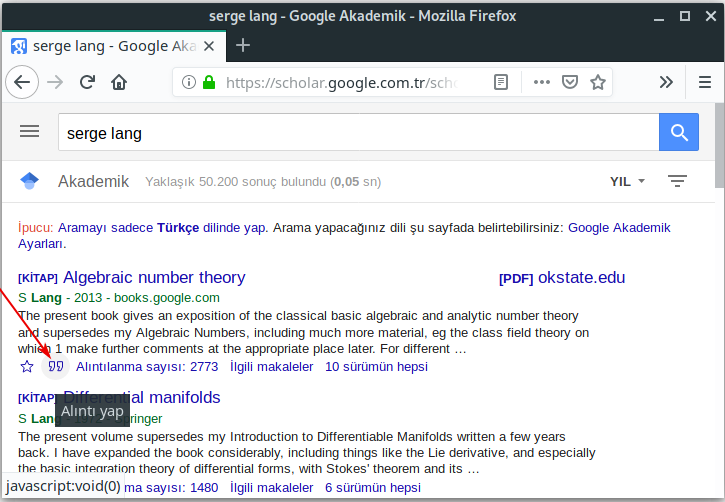
\includegraphics[width=0.33\linewidth]{images/galinti1} 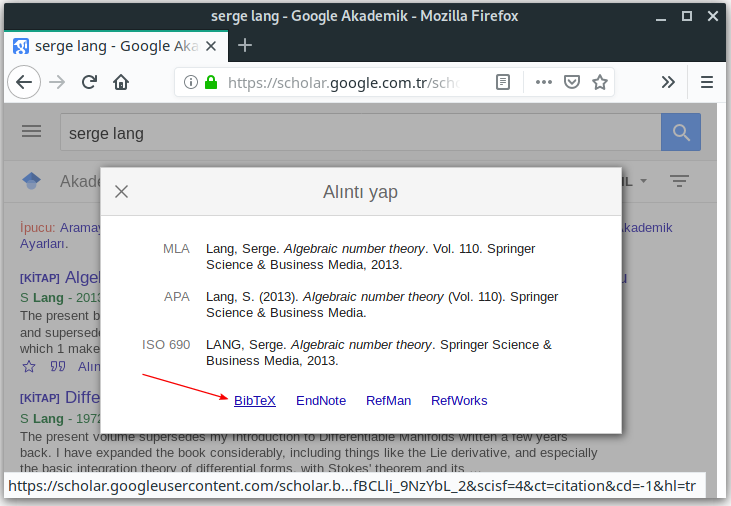
\includegraphics[width=0.33\linewidth]{images/galinti2} 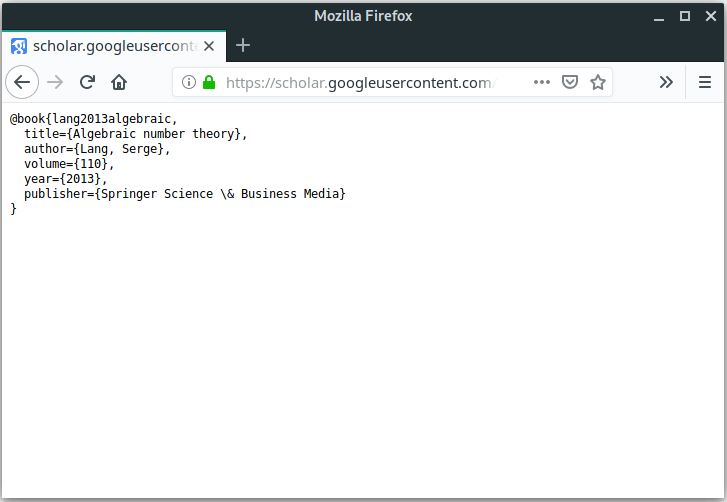
\includegraphics[width=0.33\linewidth]{images/galinti3} 

}

\caption{Google Akademikten alıntı yapma}\label{fig:fig-google}
\end{figure}

\hypertarget{dosyanux131n-hazux131rlanmasux131}{%
\subsubsection{Dosyanın hazırlanması}\label{dosyanux131n-hazux131rlanmasux131}}

Aşağıda \texttt{.bib} uzantılı bir dosya örneği gösterilmiştir.

\begin{Shaded}
\begin{Highlighting}[]
\VariableTok{@book}\NormalTok{\{}\OtherTok{lang13}\NormalTok{,}
    \DataTypeTok{title}\NormalTok{=\{Algebraic number theory\},}
    \DataTypeTok{author}\NormalTok{=\{Lang, Serge\},}
    \DataTypeTok{volume}\NormalTok{=\{110\},}
    \DataTypeTok{year}\NormalTok{=\{2013\},}
    \DataTypeTok{publisher}\NormalTok{=\{Springer Science }\CharTok{\textbackslash{}\&}\NormalTok{ Business Media\},}
\NormalTok{    \}}
\VariableTok{@article}\NormalTok{\{}\OtherTok{lamport78}\NormalTok{,}
    \DataTypeTok{title}\NormalTok{=\{Time, clocks, and the ordering of events in a}
\NormalTok{        distributed system\},}
    \DataTypeTok{author}\NormalTok{=\{Lamport, Leslie\},}
    \DataTypeTok{journal}\NormalTok{=\{Communications of the ACM\},}
    \DataTypeTok{volume}\NormalTok{=\{21\},}
    \DataTypeTok{number}\NormalTok{=\{7\},}
    \DataTypeTok{pages}\NormalTok{=\{558{-}{-}565\},}
    \DataTypeTok{year}\NormalTok{=\{1978\},}
    \DataTypeTok{publisher}\NormalTok{=\{ACM\},}
\NormalTok{\}}
\VariableTok{@manual}\NormalTok{\{}\OtherTok{Oetiker06}\NormalTok{,}
    \DataTypeTok{author}\NormalTok{ = \{Oetiker, Tobias and Partl, Hubert and Hyna, Irene}
\NormalTok{        and Schlegl, Elisabeth\},}
    \DataTypeTok{title}\NormalTok{  = \{İnce bir \{}\CharTok{\textbackslash{}LaTeXe}\NormalTok{\} Elkitabı veya, 116 dakikada}
\NormalTok{        \{}\CharTok{\textbackslash{}LaTeXe}\NormalTok{\}\},}
    \DataTypeTok{note}\NormalTok{   = \{Türkçesi: Bekir Karaoğlu\},}
    \DataTypeTok{url}\NormalTok{    = \{http://ftp.ntua.gr/mirror/ctan/info/lshort/turkish/}
\NormalTok{        lshort{-}tr.pdf\},}
    \DataTypeTok{year}\NormalTok{   = \{2006\},}
\NormalTok{\}}
\end{Highlighting}
\end{Shaded}

Bu dosyada Serge Lang'a ait bir kitap (\texttt{@book}), Leslie Lamport'a ait bir makale (\texttt{@article}) ve LaTeX için bir teknik kılavuz (\texttt{@manual}) vardır.

Her kaynağın ilk olarak \texttt{@} işaretiyle türü belirtilir. Yukarıdakilere ek olarak rapor için \texttt{@report}, tez için \texttt{@thesis}, çevrimiçi kaynaklar için \texttt{@online} kullanılır. Bunların dışındaki birçok türe LaTeX editörlerinin menü çubuğuklarında bulunan ``Kaynakça (Bibliography)'' menüsünden ulaşılabilir.

İlk girdi (\texttt{lang13}, \texttt{lamport78}, \texttt{Oetiker06}) kaynağa atıf yapmak için kullanılan anahtardır. Sonrasında gelenler de tahmin edilebileceği gibi başlık (\texttt{title}), yazar (\texttt{author}), yayıncı (\texttt{publisher}), yıl (\texttt{year}), dergi (\texttt{journal}), cilt (\texttt{volume})\ldots{} gibi kaynağı tanımlayan bilgilerdir. Bu tanımlamaların her biri eşittir işaretinden sonra iki çengelli parantez arasında yapılır (çift tırnak da kullanılabilir) ve her tanımlama (sonuncusu olsa dahi) virgülle ayrılır.

Yazar adı ya

\begin{Shaded}
\begin{Highlighting}[]
\CommentTok{author=\{Adı Soyadı\}}
\end{Highlighting}
\end{Shaded}

ya da

\begin{Shaded}
\begin{Highlighting}[]
\CommentTok{author=\{Soyadı, Adı\}}
\end{Highlighting}
\end{Shaded}

şeklinde girilmelidir ve birden fazla yazar varsa yazarlar yukarıdaki yazımdan dolayı virgülle değil \texttt{and} ile ayrılmalıdır. Yazarları ayırmak için virgül kullanırsanız yüksek ihtimalle LaTeX, yazarların adları ve soyadlarını karıştıracaktır.

Bir diğer önemli nokta özel kelimeleri yazmak için kullanılan komutları ve aksanlı harfleri iki çengelli parantez içinde yazmaktır. Örneğin ``â'' için \texttt{\{\textbackslash{}\^{}a\}} yazılmalıdır. Genel olarak sorun yaşanan karakterleri iki çengelli parantez içine yazmak gerekir.

Her tür için zorunlu olarak belirtilmesi gereken bilgiler ve isteğe bağlı bilgiler vardır. Bunların ne olduklarını tahmin etmek zor değildir. Bu konuda editörden de yararlanabilirsiniz. Örneğin, \texttt{.bib} uzantılı dosyayı açıp editörde ``Kaynakça \(\rightarrow\) Tez'' yolunu izlerseniz aşağıdaki listeyi yazdıracaktır.

\begin{Shaded}
\begin{Highlighting}[]
\VariableTok{@thesis}\NormalTok{\{}\OtherTok{ID}\NormalTok{,}
    \DataTypeTok{author}\NormalTok{ = \{author\},}
    \DataTypeTok{title}\NormalTok{ = \{title\},}
    \DataTypeTok{type}\NormalTok{ = \{type\},}
    \DataTypeTok{institution}\NormalTok{ = \{institution\},}
    \DataTypeTok{date}\NormalTok{ = \{date\},}
    \DataTypeTok{OPTsubtitle}\NormalTok{ = \{subtitle\},}
    \DataTypeTok{OPTtitleaddon}\NormalTok{ = \{titleaddon\},}
    \DataTypeTok{OPTlanguage}\NormalTok{ = \{language\},}
    \DataTypeTok{OPTnote}\NormalTok{ = \{note\},}
    \DataTypeTok{OPTlocation}\NormalTok{ = \{location\},}
    \DataTypeTok{OPTmonth}\NormalTok{ = \{month\},}
    \DataTypeTok{OPTisbn}\NormalTok{ = \{isbn\},}
    \DataTypeTok{OPTchapter}\NormalTok{ = \{chapter\},}
    \DataTypeTok{OPTpages}\NormalTok{ = \{pages\},}
    \DataTypeTok{OPTpagetotal}\NormalTok{ = \{pagetotal\},}
    \DataTypeTok{OPTaddendum}\NormalTok{ = \{addendum\},}
    \DataTypeTok{OPTpubstate}\NormalTok{ = \{pubstate\},}
    \DataTypeTok{OPTdoi}\NormalTok{ = \{doi\},}
    \DataTypeTok{OPTeprint}\NormalTok{ = \{eprint\},}
    \DataTypeTok{OPTeprintclass}\NormalTok{ = \{eprintclass\},}
    \DataTypeTok{OPTeprinttype}\NormalTok{ = \{eprinttype\},}
    \DataTypeTok{OPTurl}\NormalTok{ = \{url\},}
    \DataTypeTok{OPTurldate}\NormalTok{ = \{urldate\},}
\NormalTok{\}}
\end{Highlighting}
\end{Shaded}

Görüldüğü gibi ilk altı satır zorunlu, OPT ile başlayanlar isteğe bağlıdır. İsteğe bağlı olanlardan belirtmek istediklerinizin başında bulunan OPT'yi silip tanımlamayı yapabilirsiniz.

Editörden yararlanmanın diğer bir yolu ``Kaynakça \(\rightarrow\) Kaynakça Kaydı Ekle\ldots{}'' yolunu izlemektir. Bu yolu izlediğinizde aşağıdaki pencere açılır (örnek TeXstudio editörüne aittir).

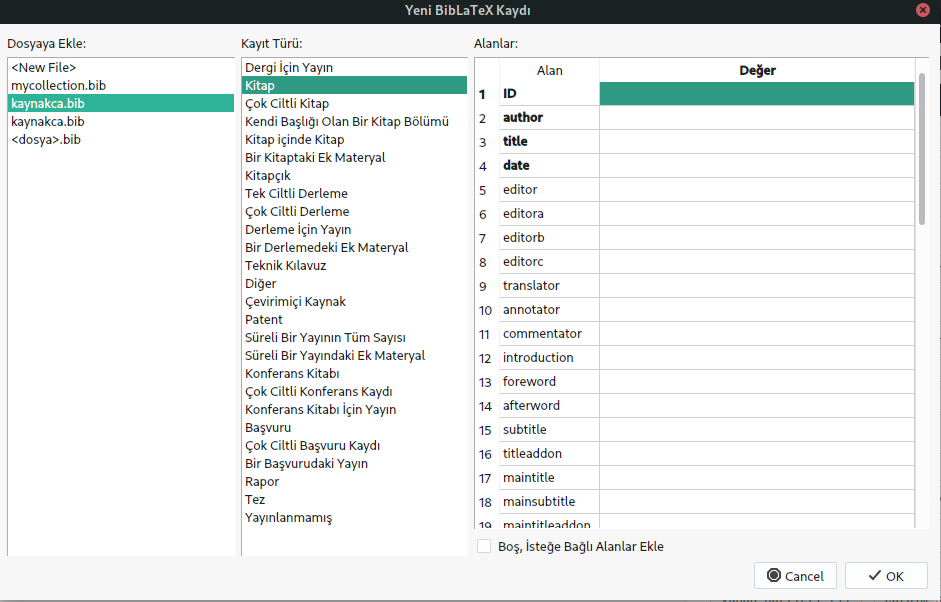
\includegraphics{images/tex-studio.png}

Pencerenin solunda kaydı eklemek istediğiniz dosyayı ve ortada kayıt türünü belirtir, sağda da kaynağın bilgilerini girersiniz. Zorunlu bilgiler en üstte yer alan kalın yazılmış olanlardır.

\hypertarget{kaynakuxe7anux131n-yazdux131rux131lmasux131}{%
\subsubsection{Kaynakçanın yazdırılması}\label{kaynakuxe7anux131n-yazdux131rux131lmasux131}}

Kaynakçayı yazdırmak için BiBTeX'i kullanacağız. BiBTeX'in LaTeX'le standart olarak geldiğini ifade etmiştik. Dolayısıyla bu programı kullanmak için ek bir şey yapmanız gerekmez.

Oluşturulan \texttt{.bib} uzantılı dosya \texttt{\textbackslash{}bibliography} komutuyla içeri aktarılır, \texttt{\textbackslash{}bibliographystyle} komutuyla da kullanılacak biçim belirtilir.

\begin{Shaded}
\begin{Highlighting}[]
\BuiltInTok{\textbackslash{}bibliographystyle}\NormalTok{\{}\ExtensionTok{\textless{}biçim\textgreater{}}\NormalTok{\}}
\BuiltInTok{\textbackslash{}bibliography}\NormalTok{\{}\ExtensionTok{\textless{}dosya\textgreater{}}\NormalTok{\}}
\end{Highlighting}
\end{Shaded}

Burada yer alan \texttt{\textless{}dosya\textgreater{}} uzantısının belirtilmesine gerek yoktur. Dosyanın \texttt{kaynakca.bib} olduğunu varsayarak, komut \texttt{\textbackslash{}bibliography\{kaynakca\}} şeklinde verilir. Kullanılabilecek biçimler \texttt{abbrv}, \texttt{acm}, \texttt{alpha}, \texttt{apalike}, \texttt{ieeetr}, \texttt{plain}, \texttt{siam} ve \texttt{unsrt}'dir. Biçimlerin nasıl çıktı verdiklerini görmek için \href{https://tr.overleaf.com/learn/latex/Bibtex_bibliography_styles}{şuraya} bakabilirsiniz.

Atıf, bütünleşik kaynakçada olduğu gibi \texttt{\textbackslash{}cite} komutuyla yapılır fakat bütünleşik kaynakçadan farklı olarak atıf yapılmayan kaynaklar yazdırılmaz. Bazı kaynakların bu kuraldan ayrı tutulması istenirse \texttt{\textbackslash{}nocite} komutu, değişkenine kaynağın anahtarı yazılarak \texttt{\textbackslash{}bibliography} komutundan önce verilmelidir.

\begin{Shaded}
\begin{Highlighting}[]
\KeywordTok{\textbackslash{}nocite}\NormalTok{\{}\ExtensionTok{\textless{}anahtar\textgreater{}}\NormalTok{\}}
\end{Highlighting}
\end{Shaded}

Eğer tüm kaynakların bu kuraldan ayrı tutulması isteniyorsa komut \texttt{\textbackslash{}nocite\{*\}} şeklinde verilmelidir.

Kaynakçanın belgeye yazılması için kaynak dosyanın derlenip, BiBTeX programının çalıştırılması ve ardından dosyanın en az iki kere daha derlenmesi gerekir. BiBTeX programı, editörde ``Araçlar \(\rightarrow\) Kaynakça'' yoluyla çalıştırılır (klavye kısa yolu F8). Aynı şey, uçbirimde sırasıyla

\begin{Shaded}
\begin{Highlighting}[]
\ExtensionTok{pdflatex}\NormalTok{ kaynakdosya}
\ExtensionTok{bibtex}\NormalTok{ kaynakdosya}
\ExtensionTok{pdflatex}\NormalTok{ kaynakdosya}
\ExtensionTok{pdflatex}\NormalTok{ kaynakdosya}
\end{Highlighting}
\end{Shaded}

komutları çalıştırılarak yapılabilir.

Aşağıda kaynak dosya örneği verilmiştir. Bu dosyayı derleyebilmeniz için içeriği yukarıda verilen \texttt{kaynakca.bib} dosyasının bu dosyayla aynı dizinde olması gerektiğini unutmayınız.

\begin{Shaded}
\begin{Highlighting}[]
\BuiltInTok{\textbackslash{}documentclass}\NormalTok{[10pt,a4paper]\{}\ExtensionTok{article}\NormalTok{\}}
\BuiltInTok{\textbackslash{}usepackage}\NormalTok{[T1]\{}\ExtensionTok{fontenc}\NormalTok{\}}
\BuiltInTok{\textbackslash{}usepackage}\NormalTok{[turkish]\{}\ExtensionTok{babel}\NormalTok{\}}
\BuiltInTok{\textbackslash{}usepackage}\NormalTok{\{}\ExtensionTok{dtk{-}logos}\NormalTok{\} }\CommentTok{\% \textbackslash{}BibTeX komutu için...}
\FunctionTok{\textbackslash{}title}\NormalTok{\{Kaynakça Yönetimi 2: }\FunctionTok{\textbackslash{}BibTeX}\NormalTok{\}}
\FunctionTok{\textbackslash{}author}\NormalTok{\{Zafer Acar\}}
\KeywordTok{\textbackslash{}begin}\NormalTok{\{}\ExtensionTok{document}\NormalTok{\}}
\FunctionTok{\textbackslash{}maketitle}
\NormalTok{Lang\textquotesingle{}ın kitabı }\KeywordTok{\textbackslash{}cite}\NormalTok{\{}\ExtensionTok{lang13}\NormalTok{\}, Lamport\textquotesingle{}un makalesi  }\KeywordTok{\textbackslash{}cite}\NormalTok{\{}\ExtensionTok{lamport78}\NormalTok{\} }
\NormalTok{ve }\FunctionTok{\textbackslash{}LaTeX}\NormalTok{\{\} için Türkçe kaynak }\KeywordTok{\textbackslash{}cite}\NormalTok{\{}\ExtensionTok{Oetiker06}\NormalTok{\} }\FunctionTok{\textbackslash{}dots}

\BuiltInTok{\textbackslash{}bibliographystyle}\NormalTok{\{}\ExtensionTok{siam}\NormalTok{\}}
\BuiltInTok{\textbackslash{}bibliography}\NormalTok{\{}\ExtensionTok{kaynakca}\NormalTok{\}}
\KeywordTok{\textbackslash{}end}\NormalTok{\{}\ExtensionTok{document}\NormalTok{\}}
\end{Highlighting}
\end{Shaded}

\hypertarget{dizin}{%
\section{Dizin}\label{dizin}}

Bilimsel bir yapıtta bulunması gereken \emph{dizin} ya da diğer adıyla \emph{indeks}, bir yapıtın kişi, konu, yer adı vb. bakımından içindekileri yer numarasıyla belirten ve yapıtın arkasında yer alan alfabetik listedir.

LaTeX'de dizin oluşturabilmek için sahanlığa

\begin{Shaded}
\begin{Highlighting}[]
\BuiltInTok{\textbackslash{}usepackage}\NormalTok{\{}\ExtensionTok{makeidx}\NormalTok{\}}
\FunctionTok{\textbackslash{}makeindex}
\end{Highlighting}
\end{Shaded}

komutları girilir. Birinci komut dizin için gerekli olan \href{http://ftp.ntua.gr/mirror/ctan/macros/latex/base/makeindx.pdf}{\textbf{makeidx}} paketini çağırır, ikinci komut ise dizinleme komutlarını etkinleştirir.

Dizinde gösterilmek istenen madde, \texttt{\textbackslash{}index} komutunun değişkeni olarak girilir:

\begin{Shaded}
\begin{Highlighting}[]
\FunctionTok{\textbackslash{}index}\NormalTok{\{\textless{}madde\textgreater{}\}}
\end{Highlighting}
\end{Shaded}

Dizin maddesi girme örnekleri aşağıda gösterilmiştir.

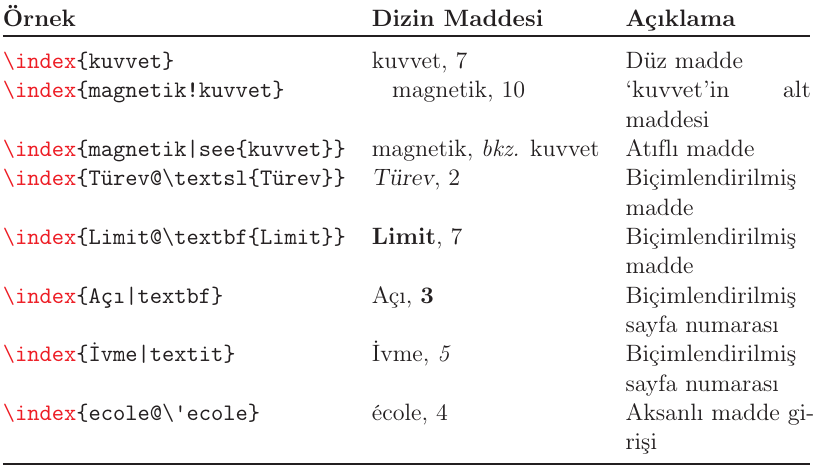
\includegraphics[width=0.9\textwidth,height=\textheight]{images/dizina.png}

LaTeX, kaynak dosyanızı derlediğinizde bu dizin maddelerini sayfa numaralarıyla birlikte, kaynak dosyayla adı aynı fakat uzantısı \texttt{.idx} olan bir dosyaya kaydeder (bu dosyaya \emph{ham dosya} denir). Bu dosyanın \texttt{makeindex} programından geçirilmesi gerekir. Bu editörde ``Araçlar \(\rightarrow\) Dizin'' yoluyla yapılır. Aynı şey uçbirimde,

\begin{Shaded}
\begin{Highlighting}[]
\ExtensionTok{makeindex}\NormalTok{ kaynakdosya}
\end{Highlighting}
\end{Shaded}

komutu girilerek yapılabilir. Dosya tekrar derlendiğinde sıralanmış dizin belgeye yazılır. Bunun için dizinin yazılması istenen yere \texttt{\textbackslash{}printindex} komutu verilir. Bu genelde, belgenin en sonunda \texttt{\textbackslash{}end\{document\}} komutundan hemen öncedir. Komutun girildiği yere LaTeX, Türkçe dil paketi ekli belgelerde ``Dizin'' başlığını oluşturur ve belgede \texttt{\textbackslash{}index} komutuyla eklenmiş maddeleri sırayla dizer.

Program, ham dosyayı işleyip dizin maddelerini abece sırasına göre dizer ve \texttt{.ind} uzantılı bir dosyaya aktarır. Ancak, Türkçe aksanlı harflerle başlayan kelimeler doğru yerde yazılmazlar. Bu harflerin doğru yere yazılması için \texttt{.ind} uzantılı dosyanın metin editörüyle açılarak elle düzenlenmesi gerekir. Ardından kaynak dosya derlenir. Elle düzeltmeden sonra tekrar \texttt{makeindex} programı çalıştırılırsa \texttt{.ind} uzantılı dosya tekrar oluşturulacağı için elle yapılan düzeltmeler bozulur. O yüzden düzeltme en son yapılmalıdır.

\begin{quote}
Aksanlı harflerle başlayan kelimelerin doğru yerde yazılmaları için aksanlı madde girme komutundan faydalanılabilir. Örneğin ``çekiç'' kelimesinin peşine \texttt{\textbackslash{}index\{czekiç@çekiç\}} komutu verilirse bu kelime doğru yerde dizilecektir. Burada yapılan sorun yaratan ``ç'' harfi yerine ``cz'' yazılmasıdır.
\end{quote}

\hypertarget{uxe7oklu-dizin}{%
\subsection{Çoklu Dizin}\label{uxe7oklu-dizin}}

Birden fazla dizin oluşturmak isterseniz (örneğin biri \emph{normal dizin} diğeri de \emph{simgeler dizini}) \href{http://ftp.cc.uoc.gr/mirrors/CTAN/macros/latex/contrib/index/index.pdf}{\textbf{index}} paketini kullanabilirsiniz. Her dizin paket eklendikten ve \texttt{\textbackslash{}makeindex} komutu sahanlıkta verildikten sonra \texttt{\textbackslash{}newindex} komutuyla tanıtılır.

\begin{Shaded}
\begin{Highlighting}[]
\BuiltInTok{\textbackslash{}usepackage}\NormalTok{\{}\ExtensionTok{index}\NormalTok{\}}
\FunctionTok{\textbackslash{}makeindex}
\FunctionTok{\textbackslash{}newindex}\NormalTok{\{normal\}\{ndx\}\{nnd\}\{Normal Dizin\}}
\FunctionTok{\textbackslash{}newindex}\NormalTok{\{simge\}\{sdx\}\{snd\}\{Simgeler Dizini\}}
\end{Highlighting}
\end{Shaded}

Komutun dört değişkeni vardır. Bunlar sırasıyla, dizin adı (örnekte \texttt{normal} ve \texttt{simge}), oluşturulacak ham dosyanın uzantısı (örnekte \texttt{.ndx} ve \texttt{.sdx}), \texttt{makeindex} tarafından ham dosyanın işlenmesiyle oluşturulan dosyanın uzantısı (örnekte \texttt{.nnd} ve \texttt{.snd}) ve son olarak \texttt{\textbackslash{}printindex} komutuyla yazdırılacak başlıktır (örnekte ``Normal Dizin'' ve ``Simgeler Dizini''). Buradaki uzantılar varsayılan \texttt{.idx} ve \texttt{.ind} uzantılardan farklı olmalıdır.

Ardından bir kelime ya da simgeyi dizine eklemek için, eklemek istenilen dizine göre \texttt{\textbackslash{}index} komutu köşeli parantezler içinde dizin adı belirtilerek kullanılır.

\begin{Shaded}
\begin{Highlighting}[]
\FunctionTok{\textbackslash{}index}\NormalTok{[normal]\{kuvvet\}}
\FunctionTok{\textbackslash{}index}\NormalTok{[simge]\{F@}\SpecialStringTok{$}\SpecialCharTok{\textbackslash{}vec}\SpecialStringTok{\{F\}$}\NormalTok{\}}
\end{Highlighting}
\end{Shaded}

Birinci komut, ``kuvvet'' kelimesini normal dizine, ikinci komut \(\vec{F}\) simgesini simgeler dizinine ekler.

Belge derlendikten sonra iki tane \texttt{\textbackslash{}makeindex} komutu uçbirimde,

\begin{Shaded}
\begin{Highlighting}[]
\ExtensionTok{makeindex}\NormalTok{ kaynakdosya.ndx }\AttributeTok{{-}o}\NormalTok{ kaynakdosya.nnd }
\ExtensionTok{makeindex}\NormalTok{ kaynakdosya.sdx }\AttributeTok{{-}o}\NormalTok{ kaynakdosya.snd }
\end{Highlighting}
\end{Shaded}

şeklinde verilir. Belgenizde dizinlerin yazılması istenen yere de

\begin{Shaded}
\begin{Highlighting}[]
\FunctionTok{\textbackslash{}printindex}\NormalTok{[normal]}
\FunctionTok{\textbackslash{}printindex}\NormalTok{[simge]}
\end{Highlighting}
\end{Shaded}

komutları verilir. Ardından belge tekrar derlenerek dizinler yazdırılır.

Çoklu dizin için diğer bir seçenek \href{https://www.ctan.org/pkg/multind}{\textbf{multind}} paketini kullanmaktır. Görece index paketine göre daha pratiktir. Sahanlığa

\begin{Shaded}
\begin{Highlighting}[]
\BuiltInTok{\textbackslash{}usepackage}\NormalTok{\{}\ExtensionTok{multind}\NormalTok{\}}
\FunctionTok{\textbackslash{}makeindex}\NormalTok{\{normal\}}
\FunctionTok{\textbackslash{}makeindex}\NormalTok{\{simge\}}
\end{Highlighting}
\end{Shaded}

komutlarıyla \texttt{normal} ve \texttt{simge} adında iki dizin tanımlanır. Yine dizine yazılması istenen maddeler \texttt{\textbackslash{}index} komutundan önce çengelli parantezler içinde dizin adı belirtilerek girilir.

\begin{Shaded}
\begin{Highlighting}[]
\FunctionTok{\textbackslash{}index}\NormalTok{\{normal\}\{kuvvet\}}
\FunctionTok{\textbackslash{}index}\NormalTok{\{simge\}\{F@}\SpecialStringTok{$}\SpecialCharTok{\textbackslash{}vec}\SpecialStringTok{\{F\}$}\NormalTok{\}}
\end{Highlighting}
\end{Shaded}

Bu defa \texttt{makeindex} programı uçbirimde

\begin{Shaded}
\begin{Highlighting}[]
\ExtensionTok{makeindex}\NormalTok{ normal}
\ExtensionTok{makeindex}\NormalTok{ simge}
\end{Highlighting}
\end{Shaded}

komutlarıyla çalıştırılır. Yine \texttt{\textbackslash{}printindex} komutları dizinlerin eklenmesi istenen yere

\begin{Shaded}
\begin{Highlighting}[]
\FunctionTok{\textbackslash{}printindex}\NormalTok{\{normal\}\{Normal Dizin\}}
\FunctionTok{\textbackslash{}printindex}\NormalTok{\{simge\}\{Simgeler Dizini\}}
\end{Highlighting}
\end{Shaded}

şeklinde verilir.

\hypertarget{dizinin-iuxe7indekiler-tablosuna-yazux131lmasux131}{%
\subsection{Dizinin İçindekiler tablosuna yazılması}\label{dizinin-iuxe7indekiler-tablosuna-yazux131lmasux131}}

Dizini İçindekiler tablosuna yazmak için \texttt{\textbackslash{}printindex} komutunun peşine \texttt{book} ve \texttt{report} sınıflarında \texttt{\textbackslash{}addcontentsline} komutu,

\begin{Shaded}
\begin{Highlighting}[]
\FunctionTok{\textbackslash{}addcontentsline}\NormalTok{\{toc\}\{chapter\}\{}\FunctionTok{\textbackslash{}indexname}\NormalTok{\}}
\end{Highlighting}
\end{Shaded}

şeklinde, \texttt{article} sınıfında ise

\begin{Shaded}
\begin{Highlighting}[]
\FunctionTok{\textbackslash{}addcontentsline}\NormalTok{\{toc\}\{section\}\{}\FunctionTok{\textbackslash{}indexname}\NormalTok{\}}
\end{Highlighting}
\end{Shaded}

şeklinde verilmelidir. Çoklu dizin oluşturulmuşsa, \texttt{book} ve \texttt{report} sınıflarında

\begin{Shaded}
\begin{Highlighting}[]
\FunctionTok{\textbackslash{}printindex}\NormalTok{\{normal\}\{Normal Dizin\}}
\FunctionTok{\textbackslash{}addcontentsline}\NormalTok{\{toc\}\{chapter\}\{Normal Dizin\}}
\FunctionTok{\textbackslash{}printindex}\NormalTok{\{simge\}\{Simgeler Dizini\}}
\FunctionTok{\textbackslash{}addcontentsline}\NormalTok{\{toc\}\{chapter\}\{Simgeler Dizini\}}
\end{Highlighting}
\end{Shaded}

şeklinde, \texttt{article} sınıfında ise komutlardaki \texttt{chapter} yazan yere \texttt{section} yazarak verilmelidir.

\backmatter

  \bibliography{book.bib,packages.bib}

\printindex

\end{document}
